%%%%%%%%%%%%%%%%%%%%%%%%%%%%%%%%%%%%%%%%%%%%%%%%%%%%%%%%%%%%%%%%%%%%%%
%
% システム最適化研究室 卒業論文テンプレート(2016 年度版)
%
%%%%%%%%%%%%%%%%%%%%%%%%%%%%%%%%%%%%%%%%%%%%%%%%%%%%%%%%%%%%%%%%%%%%%%
\AtBeginDvi{\special{pdf:tounicode 90ms-RKSJ-UCS2}}
\documentclass[a4paper,12pt,fleqn]{jarticle}
\usepackage{amsmath}
\usepackage{amsfonts}
\usepackage{ascmac}
\usepackage[dvipdfmx]{hyperref}
%\usepackage{graphicx}
%%%%%%%%%%%追加した(各自必要に応じて追加してください)%%%%%%%%%%%%%%%
\usepackage{comment}
\usepackage[dvipdfmx]{graphicx}
\usepackage{array,booktabs}
\usepackage{fancybox}
\usepackage{here}
\usepackage{slashbox}
\usepackage{url}
\usepackage{comment}
\usepackage{graphics}
%%%%%%%%%%%%%%%%%%%%%%%%%%%%%%%%%%%%%%%%%%%%%%%%%%%%%%%%%%%%%%%%%%%%%%
\textwidth      16.0cm
\textheight     25.0cm
\oddsidemargin   0.5cm
\evensidemargin  0.5cm
\topmargin      -1.0cm
\footskip        1.0cm

\renewcommand{\baselinestretch}{1.2}

%%%%%%%%%%%%%%%%%%%%%%%%%%%%%%%%%%%%%%%%%%%%%%%%%%%%%%%%%%%%%%%%%%%%%%
\begin{document}

%%%%%%%%%%%%%%%%%%%%%%%%%%%%%%%%%%%%%%%%%%%%%%%%%%%%%%%%%%%%%%%%%%%%%%
% 表紙出力(ただし卒論には綴じない.表紙は別途作成する)
%%%%%%%%%%%%%%%%%%%%%%%%%%%%%%%%%%%%%%%%%%%%%%%%%%%%%%%%%%%%%%%%%%%%%%
\pagestyle{empty}
\begin{center}
 \ \\
 \vspace{8cm}
 \begin{Large}
    {\bf 設置者の稼働時間を考慮した止水板最適設置順序の算出}\\
 \end{Large}
 \vspace{2cm}
 \begin{large}
  {\bf システム最適化研究室} \\
  {\bf 都 14-86 竹内  美紗}
 \end{large}
\end{center}

%% vspace のあとの寸法は,出来上がりイメージを見て適宜修正すること

%%%%%%%%%%%%%%%%%%%%%%%%%%%%%%%%%%%%%%%%%%%%%%%%%%%%%%%%%%%%%%%%%%%%%%
% 目次出力
%%%%%%%%%%%%%%%%%%%%%%%%%%%%%%%%%%%%%%%%%%%%%%%%%%%%%%%%%%%%%%%%%%%%%%
\newpage
\pagestyle{plain}
\pagenumbering{roman}
\tableofcontents

%%%%%%%%%%%%%%%%%%%%%%%%%%%%%%%%%%%%%%%%%%%%%%%%%%%%%%%%%%%%%%%%%%%%%%
% \chapter\documentclass[]{jreport},\documentclass[]{jbook} 環境でないため使えません
% 章は\section,節は\subsection,小節は\subsubsection
%%%%%%%%%%%%%%%%%%%%%%%%%%%%%%%%%%%%%%%%%%%%%%%%%%%%%%%%%%%%%%%%%%%%%%
\newpage
\pagenumbering{arabic}
\section{はじめに}

日本は,地震や火山の噴火など,世界的に見ても災害の非常に多い国である.そ
の中でも,大雨による被害は,我々の先祖を常に苦しめてきた.日本の急峻な地
形は,雨が降り注いでから海に到達するまでの時間を短くし,川の流れを激しく
する.山間部から流された土が下流に肥沃な大地を作って農業が盛んになる反面,
それができるまでの過程で多くの人命が危険にさらされた.

近年,日本では大雨の発生数が増加しており,甚大な被害を招いている.最近も,
$2017$ 年 $7$ 月に九州北部地方で発生した豪雨は,福岡県・大分県で $37$ 名
もの死者を出した.
%
大雨や降水量への影響に関する研究は国土交通省,気象庁,文部科学省などで広
く行われており,大雨の発生数の増加傾向には地球温暖化が影響している可能性
も指摘されている.
%
%今後,地球温暖化が進行した場合には,大雨の発生数も増加すると予測されてい
%る.
%
また, 1 時間の降水量が 50 mm 以上の短時間強雨の発生回数も増加傾向にある
\cite{集中豪雨の増加傾向と水害への対策}.以下に集中豪雨の例を挙げる.

\begin{itemize}
\item 岡崎豪雨\cite{岡崎豪雨}
\begin{itemize}
\item 2008 年 8 月 28 日から 29 日にかけて,愛知県を中心に局地的な大雨となり,各地で浸水や土砂災害が発生した.1 時間最大雨量は 146.5 mm の猛烈な雨を観測した.名古屋市の浸水が 10,000 棟,岡崎市でも 2,130 棟が浸水した.被災による死者は 2 名と甚大な被害が出た.
\end{itemize}
\end{itemize}

\begin{itemize}
\item 東海豪雨\cite{東海豪雨}
\begin{itemize}
\item 2000 年 9 月 11 日から 12 日にかけて東海地方を中心に豪雨が発生した.名古屋では 1 時間最大雨量 97 mm,東海市では 1 時間最大雨量 114 mm を記録した.茨城県から沖縄県までにおよぶ被害総計は,床上浸水 27,180 棟,床下浸水 44,111 棟,死者 10 名であった.
\end{itemize}
\end{itemize}

本研究では,このような豪雨が都市部に降り注いだ時のことを考える.
%
都市部では土地の高度利用が進み,地下街や地下室の設置が増加している.地下
街等の地下施設は,このような集中豪雨によって短時間に浸水する危険性をはら
んでおり,逃げ遅れや閉じ込め等によって財産のみならず人命までもが危険にさ
らされる可能性がある.雨の降り始めから浸水発生までの時間が短いことや地下
空間の閉鎖性を考えると,人的被害を減らすためには,適切な行動を取ることが
必要である.

このような状況を踏まえ,馬谷 \cite{馬谷さん卒論} は水害発生時の浸水対策の
1 つとして梅田地下街全域を対象とした止水板の最適設置順序の算出を行った.
しかし \cite{馬谷さん卒論} を子細に読み解くと,現実的な条件からやや乖離し
た設定が行われていたことがわかった.そこで本研究では,より現実に即した条
件,例えば止水板設置チームの稼働時間や,梅田地下街の管理施設などを考慮し
て,止水板の最適設置順序を算出することを目指す.

%%%%%%%%%%%%%%%%%%%%%%%%%%%%%%%%%%%%%%%%%%%%%%%%%%%%%%%%%%%%%%%%%%%%%%
%\newpage
%\section{章}
%\subsection{節}
%\subsubsection{小節}

%%%%%%%%%%%%%%%%%%%%%%%%%%%%%%%%%%%%%%%%%%%%%%%%%%%%%%%%%%%%%%%%%%%%%%
\newpage
\section{準備}
本章では,本研究で必要になる事項について説明する.
\subsection{数理計画問題}
数理計画問題\cite{数理計画入門}は一般に次のように表すことができる.\\
\hspace{3.0cm}目的関数:\ $f(x)$\hspace{0.2cm}$\rightarrow$\hspace{0.2cm} 最小(あるいは最大)\\
\hspace{3.0cm}制約条件:\ $x \in S$\\
ここでは,変数 $x$ は $n$ 次元のベクトルであり,目的関数 $f$ は $R^n$ ($n$ 次元実ベクトル空間) 上で定義された実数値関数である.また,制約条件を満たす $x$ を実行可能といい,その集まりである集合 $S \subseteq R^n$ を実行可能領域,実行可能解の中で目的関数が最小 (あるいは最大) となるものを最適解という.

\subsection{最適化ソルバ}
\label{subsec:solver}
最適化ソルバは,最適化問題の最適解を得るためのソフトウェアである.これを利用するためには,まず,最適化問題の定式化を行い,次に定式化した問題をモデリング言語で記述する.ここで最適化ソルバによって利用できるモデリング言語は異なることに注意する必要がある.そして,記述した問題を最適化ソルバで読み込み,内部で求解アルゴリズムを実行することによって,最適解を得る.ここで本研究で用いた最適化ソルバであるGLPK,Gurobi について説明する.
\begin{itemize}
\item GLPK\cite{GLPK}
  \begin{itemize}
  \item GLPKとは GNU\ Linear\ Programming\ Kit\ の略で,GNUが無料で配布しているソルバである.このソルバは最適化計算を行うだけでなく,AMPL で書かれたモデルとデータを用いて,LP 形式のファイルを作成することができる.
  \end{itemize}
  
\item Gurobi\cite{Gurobi}
  \begin{itemize}
  \item Gurobiとは,線形計画問題 (LP),二次計画問題 (QL),二次制約 (QCP),混合整数計画 (MIP) を解くことができるソルバの1つである.
  \end{itemize}
  本研究では,Gurobi によって計算を行っている.
\end{itemize}

\subsection{ネットワーク上でのフロー保存則}

最適化問題を定式化するためには,対象となる問題をよく観察し,それを表現す
るための数式を準備する必要がある.これは個々の問題に即して行われるべき作
業ではあるが,複数の問題に共通して現れるパターンも存在する.
%
その中でも,グラフを用いて対象を表現できる場合が多く存在する.グラフは節
点の集合 $V$ と節点間をつなぐ枝の集合 $E$ を用いて $G = (V, E)$ と表現す
ることができる.
%
\begin{figure}[htpb]
 \begin{center}
%  \includegraphics[scale=0.8, bb = 100 600 300 800, clip]{./tex_files/fig/chapter_preliminaries_fig2.pdf}
  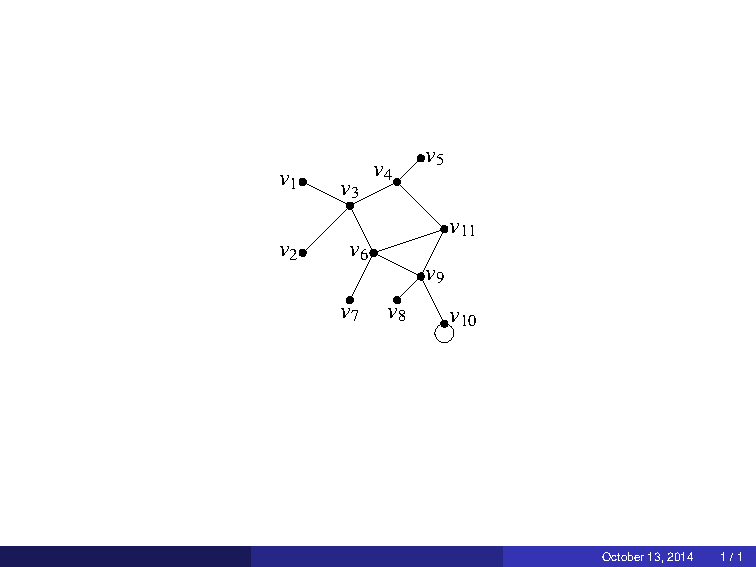
\includegraphics[scale=1.5, bb = 100 100 260 230, clip]{./fig/fig_GraphEx.pdf}
  \caption{グラフの例}
  \label{fig:Graph1}
 \end{center}
\end{figure}
%
例えば図 \ref{fig:Graph1} は
%
\begin{align*}
 V &= \{v_1, v_2, v_3, v_4, v_5, v_6, v_7, v_8, v_9, v_{10}, v_{11}\}, \\
 E &= \{ (v_1, v_3),(v_2, v_3),(v_3, v_4),(v_4, v_5),(v_4, v_{11}),(v_3, v_6), \\
 & \quad \quad (v_6, v_7),(v_6, v_9),(v_6, v_{11}),(v_8, v_9),(v_9, v_{10}),(v_9, v_{11}),
 (v_{10}, v_{10}) \}
\end{align*}
%
であるようなグラフの例である.

グラフを用いて表現できるものの一つに,ネットワーク上のフローがある.ここ
でいうネットワークとは,例えば道路網や上下水道網などのことで,そこでのフ
ローとは交通流や水の流れを表している.このようなフローを考える際には,フ
ロー保存則と呼ばれるルールを適用することが多い.
%
これは,
%
\begin{screen}
 グラフ上のフローは各節点で保存される
\end{screen}
%
という単純なものである.例えば,グラフが水道管網を表しており,枝の上を水
が流れていく場合,「節点で水漏れしない」ということがフロー保存則に対応す
る.言い換えれば,「節点に流れ込む量と節点から流れ出る量が等しい」という
ことができる,直感的にもイメージしやすいルールである.
%
ただし,フローの始点となる節点(ソース)と終点となる節点(シンク)ではこ
のルールは適用されないことに注意する.

グラフ $G = (V, E)$ 上でのフロー保存則を定式化すると,次のようになる.
%
\begin{align}
 & \sum_{(i, v) \in E} x_{iv}
 = \sum_{(v, j) \in E} x_{vj}, \quad (v \in V, \; v \not= s, t)
 \label{eq:design_network_1} \\
 %
 & \sum_{(s, j) \in E} x_{sj}
 = f \left( = \sum_{(j, t) \in E} x_{jt} \right)
 \label{eq:design_network_2} \\
 %
 & x_{ij} \ge 0, \quad ((i, j) \in E)
 \label{eq:design_network_3}
\end{align}
%
ここで $s$ はソース,$t$ はシンクを表しており,$x_{ij}$ は枝 $(i, j) \in
E$ の上を流れるフローの量,$f$ はフローの全量とする.

(\ref{eq:design_network_1}) は,ソースあるいはシンクでない節点 $v \in V$,
すなわちにフローを中継する節点に適用される式である.
%
(\ref{eq:design_network_1}) の左辺は節点 $v$ に入る枝を流れるフローの和を,
右辺は節点 $v$ から出て行く枝を流れるフローの和を表しており,これらが等し
くなるということが,フロー保存則に他ならない.フローの量は,それが連続的
に分割可能なもの(例えば水など)であれば連続変数で表現すればよいし,分割
できないものであれば整数変数で表現することになる.

また (\ref{eq:design_network_2}) の左側の等号は,ソース $s$ から流れ出る
フローの量が $f$ であることを表している.そして,フロー保存則の下ではフロー
がどこかに消えるようなことはないため,このフローは全てシンク $t$ に到達す
ることになる.それが (\ref{eq:design_network_2})の右側の等号で表現されて
いる.

最後に (\ref{eq:design_network_3}) は,フローの量が非負であることを表して
いる制約である.もしこの制約がなければ,フローの量が負になってしまう可能
性がある.

その他に,各枝にフローの容量に関する制約が付加される場合がある.これは,
例えば,水道管の直径に応じて流す事が可能な容量を定めるような場合などであ
る.その場合は,枝 $(i, j) \in E$ の容量を $c_{ij} \; (\ge 0)$ とすると,
%
\begin{align}
 x_{ij} \le c_{ij}
 \label{eq:design_network_4}
\end{align}
%
とすることができる.


%%%%%%%%%%%%%%%%%%%%%%%%%%%%%%%%%%%%%%%%%%%%%%%%%%%%%%%%%%%%%%%%%%%%%%
\newpage
\section{研究の背景と目的}
本章では本研究の背景と目的について説明する.

\subsection{背景}
\label{subsec:background}
近年,我が国では都市部において局地的・集中的な豪雨による水害が発生している.特に,1時間に 100mm を超える局地的な豪雨がしばしば観測されるようになっており,地下空間における短時間集中型の豪雨への対策が求められている.地下空間の浸水は人命にかかわる深刻な被害につながる可能性が高いため,その対策は重要な課題である\cite{地下空間における浸水対策ガイドライン}.以下は,豪雨によって地下空間に甚大な被害が出た例である.

\begin{itemize}
%\item 岡崎豪雨
  %\begin{itemize}
  %\item 2008 年 8 月 28 日から 29 日にかけて東海地方や関東地方を中心に豪雨が発生した.1 時間最大雨量は 146.5 mm の猛烈な雨を観測した.愛知県内では住宅が 5 棟全壊し,床上浸水が 2477 棟,床下浸水が 14108 棟に達した.また,農作物や道路,橋梁などにも大きな影響が出た\cite{気象災害の記録1}.
  %\end{itemize}

%\item 東海豪雨
  %\begin{itemize}
  %\item 2000 年 9 月 11 日から 12 日にかけて東海地方を中心に豪雨が発生した.名古屋では 1 時間最大雨量 97 mm,東海市では 1 時間最大雨量 114 mm を記録した.この豪雨で名古屋市及びその周辺の市町村では堤防の決壊,河川の超水により,広範囲で浸水被害が発生したほか,各地で土砂災害も発生した.床上浸水は 24610 棟に達するという甚大な被害が発生した\cite{気象災害の記録2}.
  %\end{itemize}

%\begin{itemize}
%\item 九州北部豪雨
 % \begin{itemize}
  %\item 2017 年 7 月 5 日,福岡県と大分県を中心とした九州北部で発生した集中豪雨である.九州で初めて大雨警報が発表された.最多雨量は福岡県朝倉市で 1 時間 129.5ミリを観測した.被害の状況として,倒壊した家は 7 件,床上浸水した家は 21 件あった.道路については冠水した道路は 54 箇所に上った\cite{災害時気象資料}.  
  %\end{itemize}

\item 福岡水害\cite{福岡水害国土交通省}
  \begin{itemize}
  \item 1999 年 6 月 29 日,福岡市を流れる三笠川があふれて市中心部が冠水し,博多駅や地下施設に水が流入した.1 時間雨量は 79.5 mmを観測した.
  \item 駅周辺で地下施設を持つビル 182 棟のうち,地下が浸水したビルは 71 棟に上り,そのうち地下 3 階まで浸水したビルが 3 棟,地下空間が完全に水没したビル10棟あった.地下階の総浸水面積は約 5 万m$^2$となった.
  \item 地下鉄については,道路の水が出入り口階段 5 ヶ所から流入し,最大 25 cm浸水した.この水は地下ホーム,線路へと流れ込み線路の冠水が発生した.
  \item 人的被害については 37 人の死亡,4 人の行方不明が確認された.
  \end{itemize}
\end{itemize}

このような大規模な都市型水害が,近年多発している.そのため地下空間の水害の軽減に着目した研究が多く行われている.

先行研究\cite{水工学論文集1,水工学論文集2}では,梅田の地下街を対象として,下水道施設を考慮した内水氾濫解析が行われている.具体的には,岡崎豪雨や東海豪雨を外力と設定し,雨水流出解析モデルとして下水施設および地表面の氾濫解析を同時に実施した.その結果,地下空間に流入する出入り口の場所,流入順序,流入時間,流入量を推定することができ,事前に止水活動や避難誘導が可能であることが示された.%それをもとに武田の研究\cite{武田さん卒論}では,地下空間の浸水対策として ホワイティうめだを対象とした止水板設置が検討された.

そして,\cite{水工学論文集1,水工学論文集2}をもとに,止水活動を円滑に行うための研究が行われている.例えば武田の研究\cite{武田さん卒論}では,地下空間の浸水対策としてホワイティうめだを対象とし,内水氾濫シュミレーションが行われた.外力を短時間集中豪雨とした場合に,地下街の管理者は十分な対策がとれず,人員を十分確保できないリスクや,止水板の設置途中で浸水が始まる可能性を考慮して止水板設置順序や設置タイミングなどが検討された.\cite{武田さん卒論}では,止水板の設置タイミングとして以下の $3$ つが挙げられた:

\newpage
\begin{itemize}
\item 地下への流入が始まったとき
   \begin{itemize}
   \item 先行研究 \cite{水工学論文集3}で計算された地下街での流入開始時刻をもとに,設置のタイミングを知る.
   \end{itemize}
\item 地上監視カメラより判断
   \begin{itemize}
   \item 最も越水が早いとされている泉の広場地上に監視カメラを設置することで,設置のタイミングを知る.
   \end{itemize}
\item 水位計より判断
   \begin{itemize}
   \item 最も浸水が早いとされている管渠に水位計を設定することで,設置のタイミングを知る.
   \end{itemize}
\end{itemize}
その結果,水位計によって判断した場合,止水板の設置が全て可能であり,流入量が大幅に削減できることが分かった.

\bigskip

一方,馬谷の研究\cite{馬谷さん卒論}も止水板の設置について考察しているが,\cite{武田さん卒論}では内水氾濫シュミレーションで止水板の設置順序を検討していたのに対し,馬谷はこの問題を最適化問題として定式化を行い,ソルバを用いて解くことで最適な設置順序を算出した.なお\cite{馬谷さん卒論}では,対象地区をホワイティうめだに限定するのではなく,梅田地下街全域を対象としている.具体的には表 \ref{tb:ex1} に示した条件で計算を行った.

\begin{table}[H]
  \begin{center}
    \caption{\cite{馬谷さん卒論}で設定された条件}
    \begin{tabular}{ll}
      \hline
      1 時間あたりの降雨量 & 60mm \\
      排水用ポンプ & 機能停止 \\
      雨水が流入する出入り口の数 & 24 箇所 \\
      止水板設置チーム数 & 6 チーム \\
      止水板設置チームの歩行速度 & 66 m/分\\
      降雨開始から止水板設置開始までの時間 & 60 分 \\
      止水板 1 箇所の設置に要する時間 & 3 分 \\
      %スタート地点のメッシュ番号 & 15728 \\
      \hline
    \end{tabular}
    \label{tb:ex1}
  \end{center}
\end{table}

\cite{馬谷さん卒論}では止水板を設置するチームの数や,降雨開始から止水板を設置し始めるまでの時間,設置チームの移動速度,止水板の設置に要する時間などを変化させて計算を行った.その結果として,

\begin{itemize}
\item 止水板設置チームが増えるほど水の流入時間の合計は短くなるが,ある一定の数まで増えると流入する時間の合計に変化はなくなる
\item 降雨開始から止水板設置開始の時間を遅くすると,水の流入時間の合計は遅くした時間よりも大幅に長くなる
\item 設置チームの移動速度を速くすると流入時間は短くなるが,徐々に流入時間の変化が小さくなる
\item 設置に要する時間が長くなると流入時間は長くなり,設置順序も変化する
\end{itemize}

ということがわかった.

\subsection{本研究の目的}

馬谷の研究\cite{馬谷さん卒論}では梅田地下街全域の全出入り口を対象として止水板の設置順序を算出しているが,梅田地下街には複数の管理主体が存在し,それぞれの地区に管理施設をもつ.そのため,豪雨時には,各管理主体がそれぞれの地区の管理施設に存在する流入する可能性のある出入り口に止水板を設置することになるはずである.また,\cite{馬谷さん卒論}では,止水板を設置するときに各設置チームの稼働時間は制限されていなかった.しかし,止水板の設置に要する負荷は相当大きいものであるため,設置チームの稼働時間には限界があると考えるのが自然である.

そこで本研究では,管理主体を考慮しつつ,設置チームの稼働時間に上限を設けた場合の最適な止水板設置順序を算出する.また,設置チームの稼働時間を考慮しなかった場合の最適な設置順序も算出し,これらの比較を行う.なお,本研究での最適な設置順序とは,\cite{馬谷さん卒論}と同様,止水板設置完了時刻と流入開始時刻の差の合計が最小となるような設置順序を指すものとする.

%そこで本研究では,各管理施設を考慮した最適な止水板設置順序の算出を目的とする.ここでの最適な設置順序も,止水板設置完了時刻と流入開始時刻の差の合計が最小となるような設置順序を最適な設置順序とする.
%止水板を設置するときに設置チームが少ないほど 1 チームの稼働時間が長くなり,各チームにかかる負担が大きくなってしまう.そこで本研究では,1 チームの稼働時間を 30 分に制限する条件を追加したときの最適な設置順序を算出する.この条件を追加した場合と追加していない場合の最適な設置順序を比較する.
%最適な設置順序を算出する上で,もう一つ考慮するべきものとして雨水ポンプがある.雨水ポンプとは雨が降った場合,地上に振る雨水を下水道管を通して河川に放流する役割のものである.ポンプ稼働時と停止時の場合では地下に水が流入するまでの時間や,流入する量が違ってくる.ポンプ稼働時と停止時では,最適な止水板設置順序はどのようになるかも検討する.
  



%%%%%%%%%%%%%%%%%%%%%%%%%%%%%%%%%%%%%%%%%%%%%%%%%%%%%%%%%%%%%%%%%%%%%%
\newpage
\section{止水板最適設置問題の定式化の改良}
本研究では,馬谷の研究\cite{馬谷さん卒論}に用いられた定式化に訂正と追加を加えたモデルを用いて最適化計算を行った.本章では,\cite{馬谷さん卒論}で提案されたモデルと,本研究での改良点について説明する.

\subsection{最適性の基準}
ここでは最適化モデルの目的関数を構築する上で重要な,最適性の基準について説明する.馬谷の研究\cite{馬谷さん卒論},また本研究では,推定された各出入り口への流入開始時刻を考慮した止水板の最適な設置計画を最適化問題として定式化する.そこで,最適性の基準として,各出入り口について,止水板の設置が完了するまでに水が流入した時間,すなわち
\[
 \max\{\mbox{止水板設置完了時刻} - \mbox{流入開始時刻}, 0\}
\]
を算出し,これらの和が最小になるような定式化を行う.


\subsection{定式化に用いられるネットワーク}
馬谷の研究\cite{馬谷さん卒論},また本研究では,地下空間の広がりと時間の経過を同時に表現するネットワークを利用して最適化モデルを構築している.ここでは,そのネットワークの特徴について説明する.
図 \ref{fig:nettowa-ku} は,地下街を想定したネットワークを表している.
\begin{figure}[H]
  \centering
  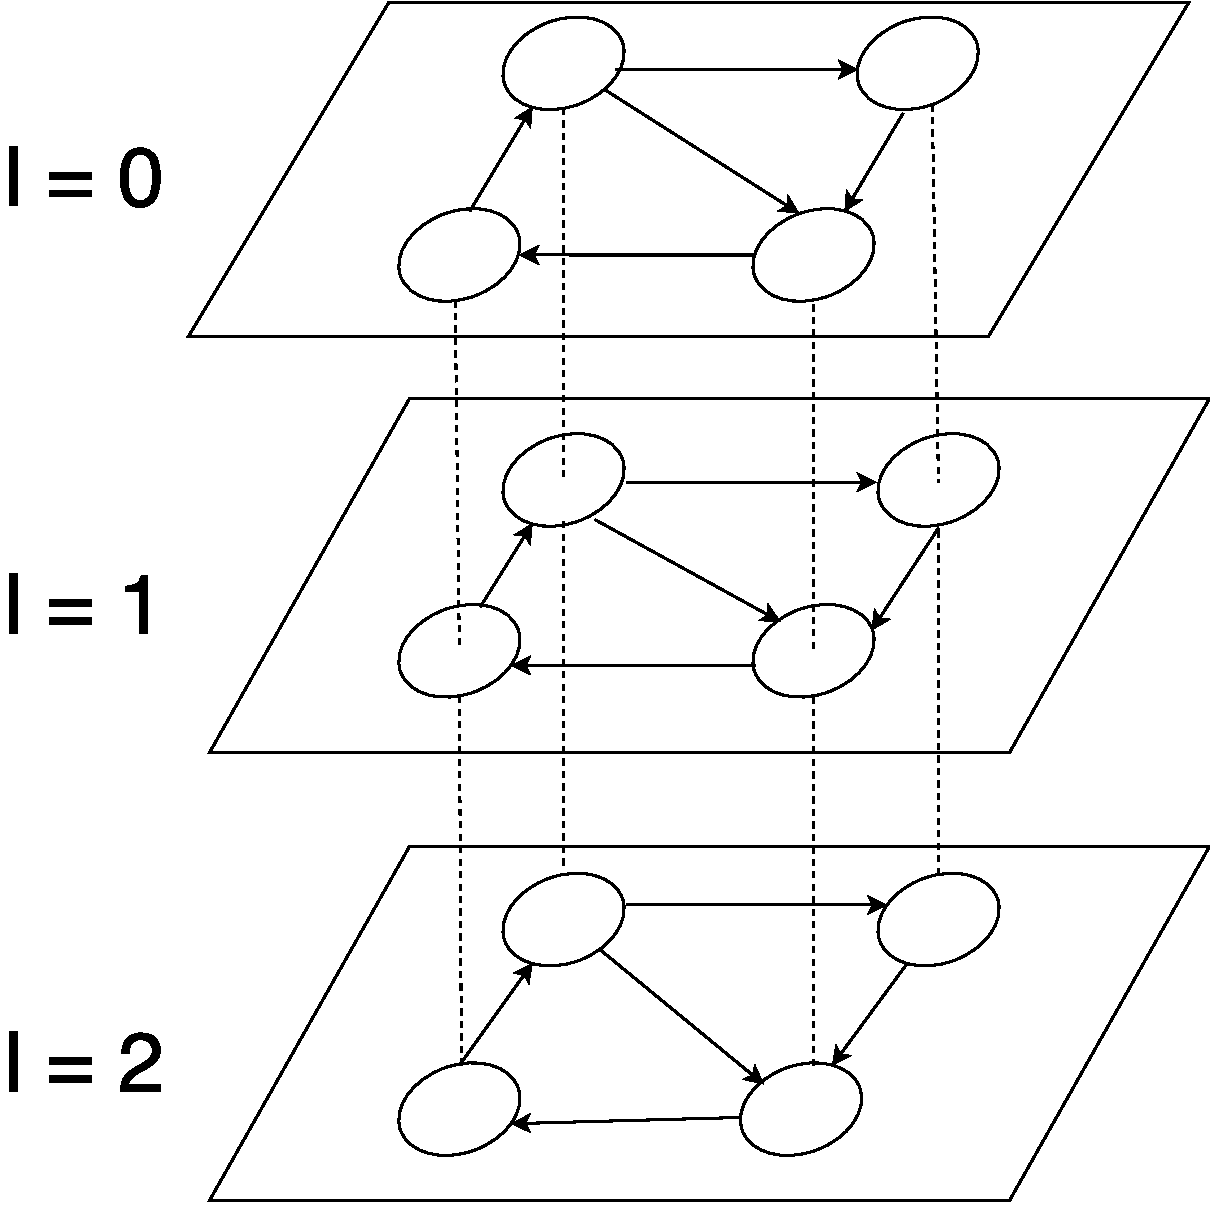
\includegraphics[keepaspectratio,scale=0.4]{nettowaku2.pdf}
  \caption{地下街のネットワーク}
  \label{fig:nettowa-ku}
\end{figure}

止水板を設置する出入り口に相当する節点を $v \in V$,出入り口間の移動に相当する枝を $(v_1,v_2) \in E$ で表す.
本研究で扱う最適化問題では,止水板を設置する各チームの動きを時間を追って表現する必要がある.そこで,このような問題を解く手段として広く用いられている時空間ネットワークを用いる.

時空間ネットワークとは,空間の形状を表すネットワークに時間軸を加えて拡張したネットワークである.すなわち時空間ネットワーク上では場所と時間が同時に表現できる.そのため,最初に出発する場所と時刻から,目的となる場所と時刻までの移動経路がリンクをたどることで求められる\cite{時空間ネットワークを用いたフライトパターンの列挙について} .

地下街を想定した時空間ネットワークを図 \ref{fig:zikuukann} に示す.
\begin{figure}[H]
  \centering
  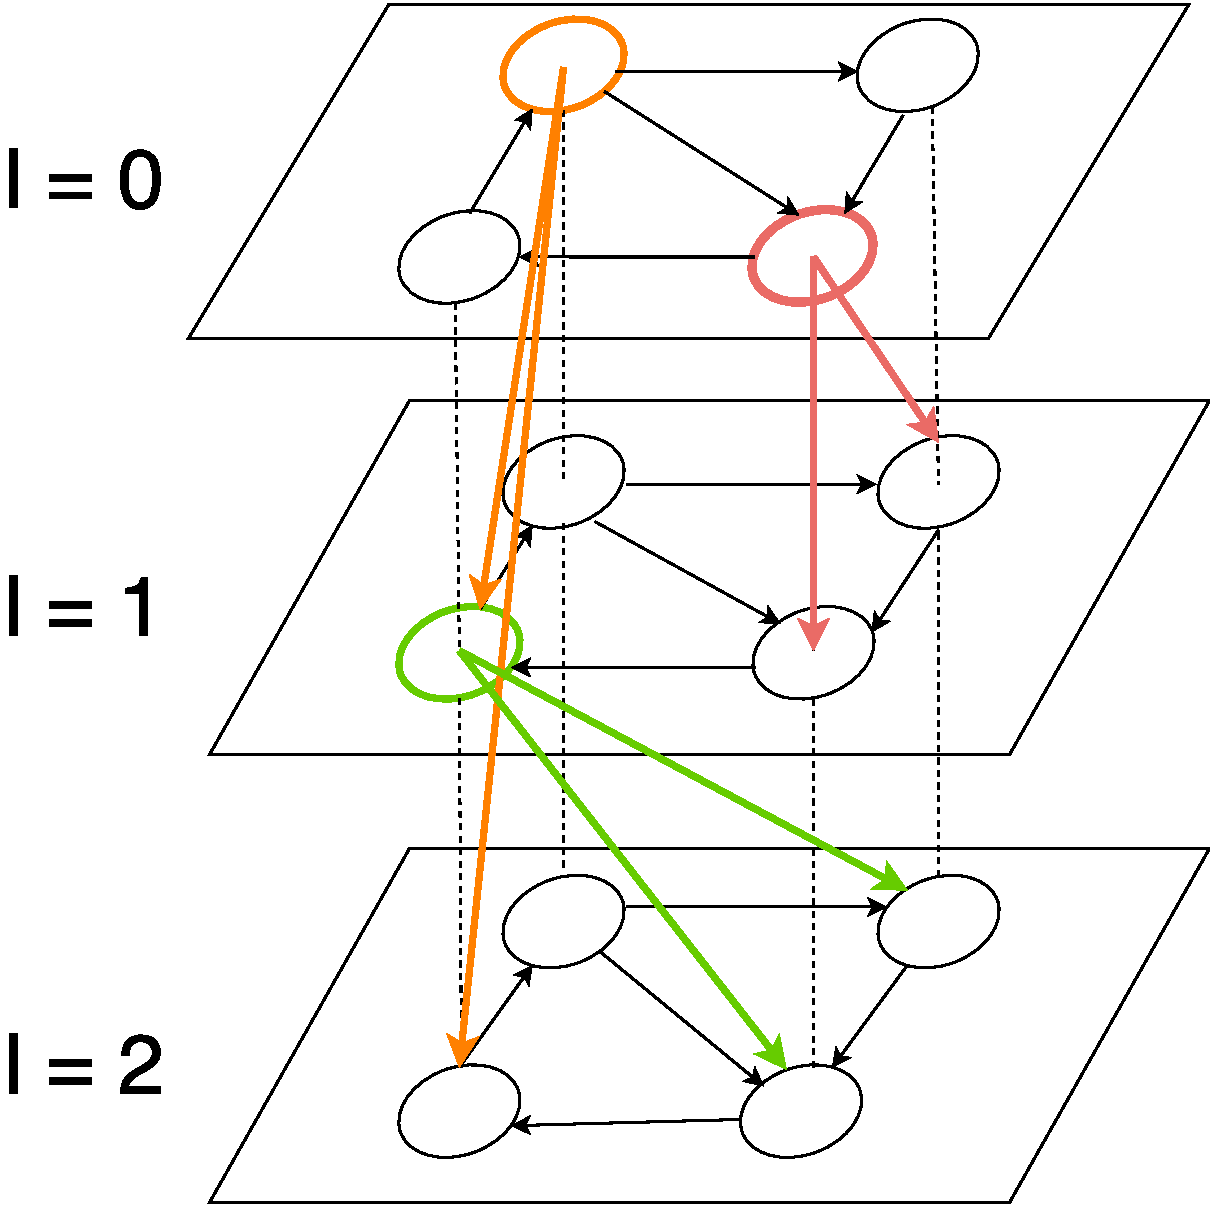
\includegraphics[keepaspectratio,scale=0.4]{nettowaku.pdf}
  \caption{時空間ネットワーク図}
  \label{fig:zikuukann}
\end{figure}

図 \ref{fig:nettowa-ku} と図 \ref{fig:zikuukann} では,止水板を設置する各チームの移動回数を $l=0,1,2,...$ とし,これを時空間ネットワークにおけるレイヤに対応させる.

\newpage

%\subsection{定式化の改良点}
%本研究では,止水板の設置のとき各管理主体の管理施設を考慮した最適な設置順序の算出を行う.また各止水板設置チームの稼働時間が 30 分になるような制約条件も追加する.

\subsection{本研究で用いる最適化問題}
本節では,本研究で止水板の設置順序を決めるために用いる最適化問題について説明する.なお,本問題は,\cite{馬谷さん卒論}で提案された問題に一部修正,追加を行ったものである(表 \ref{制約条件表}).

\begin{table}[H]
  \begin{center}
    \caption{先行研究\cite{馬谷さん卒論}からの制約条件の訂正と追加}
    \begin{tabular}{ll}\hline
      \cite{馬谷さん卒論}で提案された制約 & 制約条件 $1~7$, $9$, $10$  \\
      \cite{馬谷さん卒論}で提案された制約を修正 & 制約条件 $8$  \\
      新たに追加する制約 & 制約条件 $11$  \\\hline
    \end{tabular}
    \label{制約条件表}
  \end{center}
\end{table}


\subsubsection{集合・パラメータ・変数}
\begin{itemize}
\item 集合
  \begin{itemize}
  \item $V$ : 節点(出入り口)の集合
  \item $E$ : 枝(経路) の集合
  \item $L$ : レイヤの集合
  \item $P$ : 設置チームの集合
  \end{itemize}

\item パラメータ
  \begin{itemize}
  \item $w_e$ : 枝の重み(移動時間)
  \item $f_v$ : 節点の流入開始時刻
  \item $s$ : スタート地点
  \item $M$ : 十分大きな正の定数
  \item $u$ : 止水板設置に要する時間
  \item $a$ : 止水板設置開始時刻
  \item $l_{m}$ : 設置チームが最後に存在するレイヤ
  \item $T$ : 各設置チームの稼働時間の上限(分)
  %\item $speed$ : 設置チームの移動速度
  \end{itemize}

\item 変数
  \begin{itemize}
  \item $x_{v,l,p}$ : \ レイヤ $l$ において,設置チーム $p$ が節点 $v$ に存在するかどうかを表す $0\mathchar`-1$ 変数
    \[
    x_{v,l,p}=\left \{
    \begin{array}{l}
      1,\hspace{0.1cm} レイヤ l において,設置チーム p は節点 v に存在する\\
      0,\hspace{0.1cm} レイヤ l において,設置チーム p は節点 v に存在しない \nonumber
    \end{array}
    \right.
    \]

  \item $y_{e,l,p}$ : \ レイヤ $l$ からレイヤ $(l + 1)$ にかけて,設置チーム $p$ が枝 $e$ を通過するかどうかを表す $0\mathchar`-1$ 変数
    \[
    y_{e,l,p}=\left \{
    \begin{array}{l}
      1,\hspace{0.1cm} レイヤ l から他 (l + 1) にかけて,設置チーム p が枝 e を通過する\\
      0,\hspace{0.1cm} レイヤ l から他 (l + 1) にかけて,設置チーム p が枝 e を通過しない \nonumber
    \end{array}
    \right.
    \]

  \item $t_{l,p}$ : \ レイヤ $l$ における設置チーム $p$ の設置完了時間
  \item $\bar{t}_{l,p}$ : \ レイヤ $l$ において設置チーム $p$ が止水板を設置する出入口の流入開始時刻
  \item $d_{l,p}$ : \ レイヤ $l$ において設置チーム $p$ が止水板を設置する出入り口の設置完了時刻と流入開始時刻の差
  \end{itemize}
\end{itemize}


%\subsubsection{制約条件の改良}
%ここでは訂正と追加した制約条件について説明する.
 % \begin{description}
  %\item [制約条件 8] 各出入り口の止水板設置完了時刻
    %\begin{description}
    %\item [改善前]
   %   \begin{equation}
    %  t_{l,p}=\displaystyle\sum_{l \in L,(v_1,v_2) \in E,l < 1}y_{v_1,v_2,l,p}w_{v_1,v_2}/66.0+lu \quad (l \in L,p \in P,l \geq 1)
     %   \label{eq:Installingtime2}
      %\end{equation}
    %\end{description}
      
    %式 (\ref{eq:Installingtime2}) は馬谷の研究で使われていた改良前の制約条件である.この式 (\ref{eq:Installingtime2}) で例を挙げる.設置チーム $v_1,v_2$ で出入り口 $5$ 箇所に止水板を設置する場合を想定する.設置チーム $v_1$ は $3$ 箇所,$v_2$ は $2$ 箇所に設置すると考えるとレイヤは $3$ 必要となる.式 (\ref{eq:Installingtime2}) の $lu$ の部分は存在するレイヤの数に設置に要する時間をかけたものである.設置チーム $v_2$ は $2$ 箇所しか設置しないのでレイヤ $3$ では,どこにも設置していないことになる.しかし,この式では設置の有無にかかわらず,レイヤの存在している数だけ設置に要した時間が足されている.

    %そこで次のように改善した.
    %\begin{itemize}
    %\item 改善後
    %\begin{equation}
     % t_{l,p}=\displaystyle\sum_{l \in L,(v_1,v_2) \in E,l < 1}y_{v_1,v_2,l,p}w_{v_1,v_2}/speed + (\displaystyle\sum_{v \in V,l \in L,l \geq L,l \leq 1}x_{v,l,p}) * u
      %  \quad (l \in L,p \in P,l \geq 1)\label{eq:InstallingTime}
      %\end{equation}
      %\begin{itemize}
    %\item 改善点 :
    
    %$lu$ を $(\displaystyle\sum_{v \in V,l \in L,l \geq L,l \leq 1}x_{v,l,p}) * u$ に改善したことで,止水板を設置した数のみ設置に要した時間が足されるようになった.
      %\item [改善点 2]
       % $speed$ としている部分は移動速度を表しており,改善前に移動速度を変化させるためにはモデルファイルでの変更が必要だった.改善後ではデータファイルでの変更で移動速度を変えることができるようになった.
        %\end{itemize}
      %\end{itemize}
    %\end{itemize}
    
%  \item [制約条件 11] 各設置チームの稼働時間の制限
 %   \begin{equation}
%      t_{l_{m},p} \geq 30 \quad (p \in P)
%      \label{eq:Timelimit}
%    \end{equation}

%    式 (\ref{eq:Timelimit}) を制約条件に追加するまでは各チームの稼働時間は無制限であった.これを追加することによって各チームの稼働時間が $30$ 分に制限される.
%  \end{description}

%  本研究では,この $2$ つの改善を踏まえた制約条件を用いて計算を行っていく.


  \subsubsection{制約条件}
  本研究で用いる制約条件について説明する.
\begin{description}

\item [制約条件 1] 全止水板設置チームはレイヤ $0$ ではスタート地点に存在する
  \begin{equation}
    x_{s,0,p}=1 \quad (p \in P)\label{eq:Initialposition}
  \end{equation}

\item [制約条件 2] 全出入り口にはいずれかの設置チームが 1 度だけ存在する ($=$ 全出入り口に止水板が設置される)
  \begin{equation}
    \displaystyle \sum_{l \in L, p \in P, l \geq 1}x_{v,l,p}=1 \quad (v \in V)\label{eq:AllWaterstop}
  \end{equation}

\item [制約条件 3] 各設置チームはそれぞれのレイヤで高々 $1$ つの節点 $v$ に存在する
  \begin{equation}
    \displaystyle \sum_{v\in V}x_{v,l,p}\leq 1 \quad (l \in L, p \in P)\label{eq:OneByOne}
  \end{equation}

\item [制約条件 4] いずれかのレイヤでいずれかの設置チームが $1$ 度だけ節点 $v$ に移動する
  \begin{equation}
    \displaystyle \sum_{(\bar{v},v)\in e,l \in L,p \in P,l \geq 1}y_{\bar{v},v,l-1,p}=1 \quad (v \in V)\label{eq:SequentialInstall}
  \end{equation}

\item [制約条件 5] 枝と節点の関係性 1\\
  レイヤ $(l - 1)$ から レイヤ $l$ にかけて,止水板設置チーム $p \in P$ が節点 $v_1$ から $v_2$ に移動する場合を考える.
  $0\mathchar`-1$ 変数 $x_{v_1,l,p}$ と $y_{v_1,v_2,l-1,p}$ の組み合わせのうち 可能なものは以下のとおりである :
\newpage
  \begin{itemize}
  \item 止水板設置チーム $p_1$ が $v_1$ に存在すると時
    \begin{itemize}
    \item $x_{v_1,l-1,p}=1, y_{v_1,v_2,l-1,p}=0$ の場合
    \item $x_{v_1,l-1,p}=1, y_{v_1,v_2,l-1,p}=0$ の場合
    \end{itemize}
    
  \item 止水板設置チーム $p_1$ が $v_1$ に存在しな時
    \begin{itemize}
    \item $x_{v_1,l-1,p}=0, y_{v_1,v_2,l-1,p}=0$ の場合
    \end{itemize}
  \end{itemize}

  これらの条件を満たすために式 (\ref{eq:UsingEdge1})のように定式化を行う.
  \begin{equation}
    x_{v_1,l-1,p}\geq y_{v_1,v_2,l-1,p}
    \quad ((x_1,v_2)\in E,l \in L,p \in P,l \geq 1)
    \label{eq:UsingEdge1}
  \end{equation}
  
\item [制約条件 6] 枝と節点の関係性 2\\
  本制約では到着する節点 $v_2$ について場合分けを行う.
  $0\mathchar`-1$ 変数 $x_{v_2,l,p}$ と $y_{v_1,v_2,l-1,p}$ の組み合わせうち可能なものは以下の通りである :
  \begin{itemize}
  \item 止水板設置チーム $p_2$ が $v_2$ に存在する場合
    \begin{itemize}
    \item $x_{v_2,l,p}=1, y_{v_1,v_2,l-1,p}=0$ の場合
    \item $x_{v_2,l,p}=1, y_{v_1,v_2,l-1,p}=1$ の場合
    \end{itemize}
  \item 止水板設置チーム $p_2$ が $v_2$ に存在しない場合
    \begin{itemize}
    \item $x_{v_2,l,p}=0, y_{v_1,v_2,l-1,p}=0$ の場合
    \end{itemize}
  \end{itemize}

  これらの条件を満たすために式(\ref{eq:UsingEdge2})のように定式化を行う.
  \begin{equation}
    x_{v_2,l,p}\geq y_{v_1,v_2,l-1,p} \quad ((v_1,v_2)\in E,l \in L,p \in P,l \geq 1)\label{eq:UsingEdge2}
  \end{equation}

\item [制約条件 7] 枝と節点の関係性 3\\
  制約条件 5 と制約条件 6 では 3 つの変数が存在する.その 3 つの変数を場合分けすると 8 つの場合が考えられるが以下の場合のみ制約条件 5 と制約条件 6 では満たされていない.
  \begin{itemize}
  \item $x_{v_1,l,p}=1, x_{v_2,l,p}=1, y_{v_1,v_2,l-1,p}=0$
  \end{itemize}
  この場合を満たすために式(\ref{eq:UsingEdge3})のように定式化を行う.
  \begin{equation}
    x_{v_1,l-1,p}+x_{v_2,l,p}-y_{v_1,v_2,l-1,p} \geq 1
    \quad ((v_1,v_2) \in E,l \in L,p \in P, l \geq 1)\label{eq:UsingEdge3}
  \end{equation}

\item [制約条件 8] 各出入り口の止水板設置完了時刻\\
  変数$y_{v_1,v_2,l,p}$ を用いると,出入り口間の移動時間 $t_{l,p}$ は式(\ref{eq:InstallingTime}) のように書くことができる
  %\begin{equation}
   % t_{l,p}=\displaystyle\sum_{l_ \in L,(v_1,v_2)\in E,l < 1}y_{v_1,v_2,l,p}w_{v_1,v_2}/66.0+(l*u)
    %\quad (l \in L,p \in P,l \geq 1)\label{eq:Installingtime}
  %\end{equation}
  \newpage
  \begin{equation}
    t_{l,p}=\displaystyle\sum_{l \in L,(v_1,v_2) \in E,\bar{l} < l}y_{v_1,v_2,l,p}w_{v_1,v_2}/66.0 + u \displaystyle\sum_{v \in V,l \in L,l \geq L,l \leq 1}x_{v,l,p}
    \quad (l \in L,p \in P,l \leq L)\label{eq:InstallingTime}
  \end{equation}
  ここで,枝の重み $w_{v_1,v_2}$ は各出入り口間の移動距離を表している.また,ここでは各設置チームが分速 $66.0$m (時速 4 km に相当) で歩行することを想定している.

  次に示している式(\ref{eq:Installingtime3})は訂正前の制約条件 8 である.
  \begin{equation}
    t_{l,p}=\displaystyle\sum_{l_ \in L,(v_1,v_2)\in E,\bar{l} < l}y_{v_1,v_2,l,p}w_{v_1,v_2}/66.0+lu
    \quad (l \in L,p \in P,l \geq 1)\label{eq:Installingtime3}
  \end{equation}
  
  \cite{馬谷さん卒論} で提案されていた制約条件 8 では,式 (\ref{eq:Installingtime3}) に示したように $u \displaystyle\sum_{v \in V,l \in L,l \geq L,l \leq 1}x_{v,l,p}$ の部分が $lu$ となっていた.しかしこれは誤りである.以下,そのことを説明するため例を挙げる.設置チーム $p_1,p_2$ の 2 チームで 5 箇所の出入り口に止水板を設置する場合を想定する.例えば設置チーム $p_1$ は $3$ 箇所,$p_2$ は $2$ 箇所に設置するならば, 3 枚のレイヤが必要となる.しかし式 (\ref{eq:Installingtime3}) の項 $lu$ は単に存在するレイヤの数に設置に要する時間を乗じたものである.すると設置チーム $p_2$ は $2$ 箇所しかないにもかかわらず,3 箇所の出入り口に止水板を設置しただけの時間が加えられえてしまう.つまり,式 (\ref{eq:Installingtime3})では,設置の有無にかかわらず,レイヤの存在している数だけ設置に要した時間が足されていた.これを式 (\ref{eq:InstallingTime}) のように修正することにより,各チームが設置した止水板の数に応じた設置時間だけが加えられるようになった.

  
\item [制約条件 9] 流入開始するまでの時間\\
  本制約では設置チーム $p \in P$ がレイヤ $l$ において止水板を設置する出入り口に,雨水が流入する時間を求めている.ただし,降雨開始後 $a$ 分の時点を時刻 $0$ ($=$ 止水板の設置開始時刻) と定めている.これは雨が降り始めても,管内水位が上昇し始め,地下出入り口の地盤高に達するまでに時間を要するためである.この条件は\\式 (\ref{eq:IdealInstllingTime}) で表すことができる.
  \begin{equation}
    \bar{t}_{l,p} = \displaystyle\sum_{v \in V}x_{v,l,p}(f_v- a)
    \quad(l \in L,p \in P,l \geq 1)\label{eq:IdealInstllingTime}
  \end{equation}

\item [制約条件 10] 止水板設置完了時刻と流入開始時刻の差\\
  本制約では,設置チーム$p \in P$ がレイヤ $l$ で止水板を設置する出入り口において,止水板設置完了時刻と流入開始時刻の差がどの程度あるかを求めている.これは式 (\ref{eq:DelayTime}) のように表すことができる.
  \begin{equation}
    d_{l,p}\geq t_{l,p}-\bar{t}_{l,p}-M(1- \sum_{v \in V}x_{v,l,p})
    \quad (l \in L,p \in P,l \geq 1)\label{eq:DelayTime}
  \end{equation}

  レイヤ $l$ のとき,設置チームが出入り口 $v$ に止水板を設置しているかどうかの場合分けを行う.

  \begin{itemize}
  \item $x_{v,l,p} = 1$ となるような $v$ が存在しないとき : $d_{l,p} \geq t_{l,p} - \bar{t}_{l,p} - M$
    \begin{itemize}
    \item $M$ は十分大きな正の値であるため $t_{l,p}$,$\bar{t}_{l,p}$ がどんな値であろうと常に負の値となる.つまり,$d_{l,p} \geq 0$であるため事実上意味を持たない制約となる.
    \end{itemize}

  \item $x_{v,l,p} = 1$ となるような $v$ が存在するとき : $d_{l,p} \geq t_{l,p} - \bar{t}_{l,p}$
    \begin{itemize}
    \item (止水板設置チームの設置完了時間) $-$ (流入開始時刻) を表しており,この値が負であれば流入開始時刻に間にあっているので流入時間は $0$,値が正であれば流入開始時刻に間に合わなかった時間を算出する.
    \end{itemize}
  \end{itemize}
%\end{description}

\item [制約条件 11] 各設置チームの稼働時間の制限\\
  この制約条件は各設置チームの稼働時間を制限している.
    \begin{equation}
      t_{l_{m},p} \leq T \quad (p \in P)
      \label{eq:Timelimit}
    \end{equation}

    この制約条件を追加するまでは各チームの稼働時間は無制限であった.これを追加することによって各チームの稼働時間が $T$ 分に制限される.
  \end{description}

\subsubsection{目的関数}
本研究の目的関数は各出入り口の設置完了時刻と流入開始時刻の差の合計が最小になる値を目的関数とする.\\
\\
\ minimize \quad $\displaystyle\sum_{l \in L,p \in P,l \geq L}d_{lp}$

  

  

%%%%%%%%%%%%%%%%%%%%%%%%%%%%%%%%%%%%%%%%%%%%%%%%%%%%%%%%%%%%%%%%%%%%%%
\newpage
\section{数値実験}
\label{sec:num_ex}

本章では,前章で提案した数理計画モデルと,梅田地下街の流入データを用いて
様々な状況下での止水板の設置について行った実験内容と結果について述べる.

\subsection{実験条件と実験環境}

ここでは,止水板の設置順序を算出する対象として,梅田地下街のホワイティう
めだを取り上げる.\cite{岡部} によると,梅田地下街において,集中豪雨時に
越水の危険のある出入り口はホワイティうめだ周辺に多いことがわかっている.
%
本研究では,管理区分にも配慮し,ホワイティうめだが管轄する出入り口につい
て,最適な設置順序を考察することとした.その際,各出入り口の越水の有無,
また越水する場合にはどのタイミングで越水が始まるかについては,\cite{岡部}の
研究で得られたデータを利用した.

本実験で用いた計算環境と使用したソルバを表 \ref{計算環境},基礎となる条件
を表\ref{tb:ex1}に示す.なお,本研究では,$1$ 時間($=3600$ 秒)経過しても
計算が終わらなかった場合は,その時点で得られている最良の暫定解を最適解と
解釈することとした.

\begin{table}[H]
  \begin{center}
    \caption{計算環境}
    \begin{tabular}{cc}\hline
      OS      & Microsoft Windows 10 Home \\
      CPU     & Intel(R) Core(TM) i7-6600U CPU @ 2.60GHz 2.81GHz \\
      メモリ  & 16.0GB \\
      ソルバ  & Gurobi Optimizer \\\hline
    \end{tabular}
    \label{計算環境}
  \end{center}
\end{table}

%\subsection{実験 1}
%実験 $1$ で設定した条件は表 \ref{tb:ex1} のとおりである.

\begin{table}[H]
  \begin{center}
    \caption{基礎となる条件}
    \begin{tabular}{ll}
      \hline
      1 時間当たりの降雨量 & 120mm \\
      排水用ポンプ & 稼動 \\
      雨水が流入する出入り口の数 & 21 箇所 \\
      止水板設置チーム数 & 2 $~$ 6 チーム \\
      止水板設置チームの歩行速度 & 66 m/分 \cite{移動速度}\\
      降雨開始から止水板設置開始までの時間 & 64 分 \\
      止水板 1 箇所の世知に要する時間 & 5 分 \\
      スタート地点のメッシュ番号 & 15728 \\
      1 チームの稼働時間の制限 & 30 分 \\
      \hline
    \end{tabular}
    \label{tb:ex1}
  \end{center}
\end{table}

\subsection{実験内容}

本章では,以下の実験を行う:
%
\begin{itemize}
 \item 実験 1: 止水板の設置に必要な設置チーム数の算出
       \begin{itemize}
	\item 止水板設置チームの稼働時間に上限がある状況下で,越水する(で
	      あろう)全ての出入り口に止水板を設置するために必要な設置チー
	      ム数を算出する.
       \end{itemize}
 \item 実験 2: 設置開始時刻と流入時間の合計の関係(稼働時間に上限がある場合)
       \begin{itemize}
	\item 設置開始時刻が遅くなれば,各出入り口からの流入時間の合計は
	      大きくなるが,この関係を定量的に評価する.
       \end{itemize}
 \item 実験 3: 設置チーム数と流入時間の合計の関係(稼働時間に上限がない場合)
       \begin{itemize}
	\item 稼働時間に上限がない場合,設置チーム数が少なくとも全ての出
	      入り口に止水板を設置することができるが,流入時間の合計は大
	      きくなるはずである.この関係を定量的に評価する.
       \end{itemize}
\end{itemize}

\subsection{実験 1: 止水板の設置に必要な設置チーム数の算出}

本節では,止水板設置チームの稼働時間に上限がある状況下で,\cite{岡部} の
データで越水するとされる全ての出入り口に止水板を設置するために必要な設置
チーム数を算出する.ここでは,以下の条件で計算を行う:
%
\begin{itemize}
 \item 止水板設置開始時刻: 64 分
 \item 設置チーム数: 2, 3, 4, 5, 6 チーム
 \item 設置チームの稼働時間の上限: 30, 40, 50, 60 分
\end{itemize}
%
ここで,止水板設置開始時刻の 64 分とは,\cite{岡部} で想定される豪雨
(120mm/hr)が降り始めてから,ホワイティうめだの出入り口で最初に越水が始
まるとされる時刻である.

また,実験ケースの組合せとしては,設置チーム数が $5$ 通り,稼働時間の上限
が $4$ 通りなので合計 $5 \times 4 = 20$ 通りあるが,最適化計算が合理的に
不要であるとわかるケースについては,最適化計算を行わなかった.
%
例えば,設置チーム数を $6$ に限定するとき,稼働時間の上限が $30$ 分で対象
となる全ての出入り口に止水板を設置することができるとわかれば,上限がそれ
より大きい$40, 50, 60$ 分の場合にも設置可能なはずである.このようなケー
スについては,最適化計算を省略している.

\subsubsection{実験結果}

\begin{table}[H]
 \begin{center}
  \caption{設置チーム数・設置チームの稼働時間上限と設置可能性の関係}
  \begin{tabular}{l|cccc}\hline
   \backslashbox{チーム数}{稼働時間} & 30 & 40 & 50 & 60\\\hline
   6 & 可能 & 可能 & 可能 & 可能\\
   5 & 暫定解なし & 可能 & 可能 & 可能\\
   4 & 不可能 & 可能 & 可能 & 可能\\
   3 & 不可能 & 不可能 & 暫定解なし & 可能\\
   2 & 不可能 & 不可能 & 不可能 & 不可能\\\hline
  \end{tabular}
  \label{64分制限時間変化}
 \end{center}
\end{table}

計算結果を表 \ref{64分制限時間変化} に示す.表 \ref{64分制限時間変化} で
の「可能」「不可能」「暫定解なし」はそれぞれの以下の意味である:
%
\begin{itemize}
 \item 「可能」:設置チームが稼働時間の上限を守りながら,越水するとされる
       全ての出入り口に止水板を設置することができる.
 \item 「不可能」:設置チームが稼働時間の上限を守りながら,越水するとされる
       全ての出入り口に止水板を設置することができない.
 \item 「暫定解なし」:最適化計算によって,所定の時間(3600 秒)内に暫定
       解を得ることができなかった.これは,「可能」・「不可能」を判断で
       きるような結果を得られなかったことに相当する.
\end{itemize}

\subsubsection{考察}

本実験からわかるのは次のことである:
%
\begin{itemize}
 \item 設置チーム数が $6$ のときは,稼働時間の上限が(最短の)$30$ 分であっ
       ても,越水する全て出入り口に止水板を設置可能である.
 \item 設置チーム数が $5$ のときは,稼働時間の上限が $40$ 分以上であれば,
       越水する全て出入り口に止水板を設置可能である.また,今回の実験で
       は,稼働時間の上限が $30$ 分の場合に設置可能であるかどうかは判定
       することができなかった.
 \item 設置チーム数が $4$ のときは,稼働時間の上限が $40$ 分以上であれば
       越水する全て出入り口に止水板を設置可能,$30$ 分の場合には設置不可
       能であることがわかった.
 \item 設置チーム数が $3$ のときは,稼働時間の上限が $60$ 分以上であれば,
       越水する全て出入り口に止水板を設置可能である.また,今回の実験で
       は,稼働時間の上限が $50$ 分の場合に設置可能であるかどうかは判定
       することができなかった.さらに,$40$ 分以下の場合には設置不可能で
       ある.
 \item 設置チーム数が $2$ のときは,稼働時間の上限が(最長の)$60$ 分で
       あっても,越水する全て出入り口に止水板を設置することはできない.
\end{itemize}

\subsection{実験 2: 設置開始時刻と流入時間の合計の関係}

ここでは,設置開始時刻と流入時間の合計の関係について調べるための実験を行
う.

一般に,設置開始時刻が遅くなれば,各出入り口からの流入時間の合計は大きく
なるはずである.ここでは,この関係を定量的に評価するために,以下の条件で
計算を行う:
%
\begin{itemize}
 \item 止水板設置開始時刻: 43, 57, 64 分
 \item 設置チーム数: 6 チーム
 \item 設置チームの稼働時間の上限: 30 分
\end{itemize}

ここで,$3$ 種類の止水板設置開始時刻について説明する.
%
\ref{subsec:background} 節でも述べたように,先行研究 \cite{武田さん卒論}
では,止水板設置のタイミングとして,「水位計より判断」した時間,「地上監
視カメラより判断」した時間,「地下への流入が始まった」時間の $3$ 種類が
挙げられている.ここでの実験設定では,これら $3$ つの時間が,それぞれ
$43$, $57$, $64$ 分となっている.

\subsubsection{実験結果}

それぞれの設置開始時刻における各設置チームの最適な移動経路,すなわち最適
な止水板の設置順序は図 \ref{fig:43min_6team_lim30min_},
\ref{fig:57min_6team_lim30min_}, \ref{fig:64min_6team_lim30min_} の通りで
ある.

\begin{figure}[htpb]
 \begin{center}
  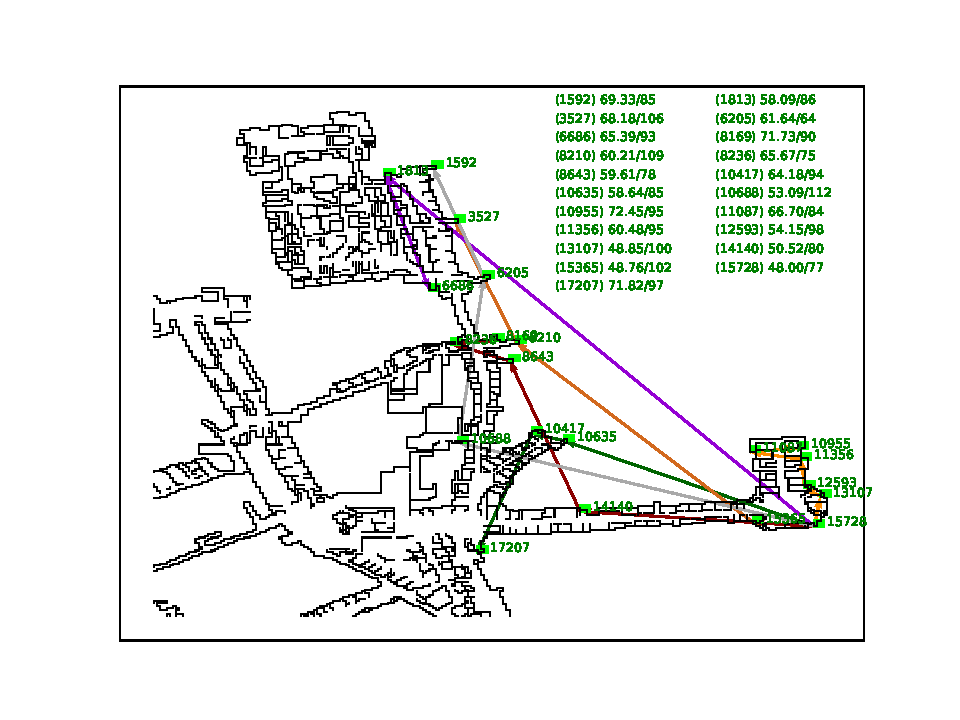
\includegraphics[width=8cm,trim=100 50 100 50]{fig/43min_6team_lim30min.pdf}
  \caption{設置開始時刻 43 分,設置チーム数 6,稼働時間上限 30 分での最
  適な止水板設置順序}
  \label{fig:43min_6team_lim30min_}
 \end{center}
\end{figure}

\begin{figure}[htpb]
 \begin{center}
  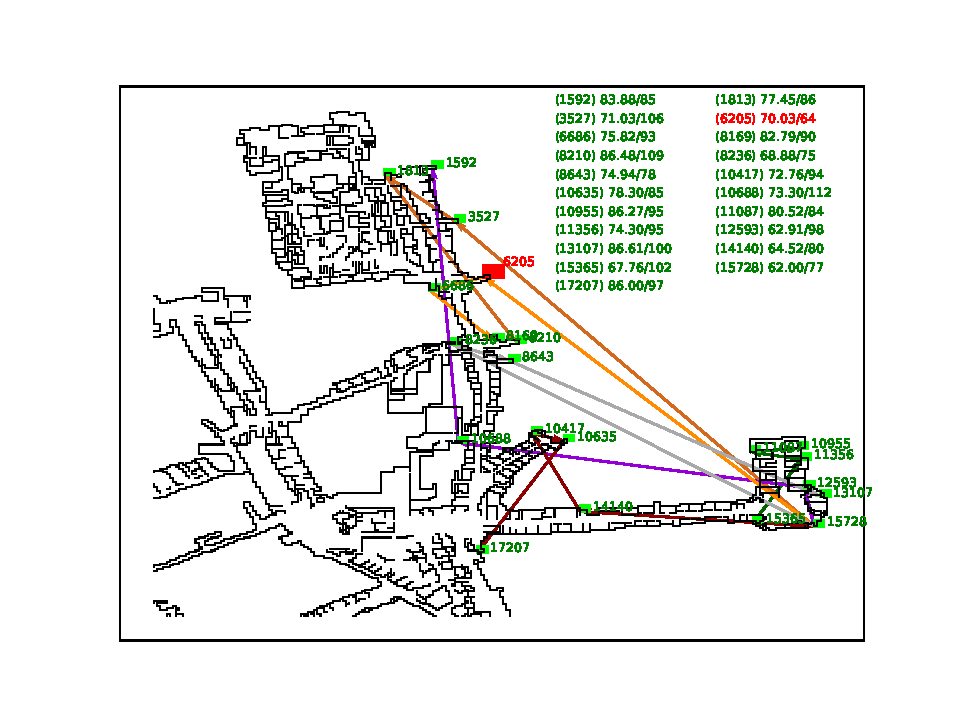
\includegraphics[width=8cm,trim=100 50 100 50]{fig/57min_6team_lim30min.pdf}
  \caption{設置開始時刻 57 分,設置チーム数 6,稼働時間上限 30 分での最
  適な止水板設置順序}
  \label{fig:57min_6team_lim30min_}
 \end{center}
\end{figure}

\begin{figure}[htpb]
 \begin{center}
  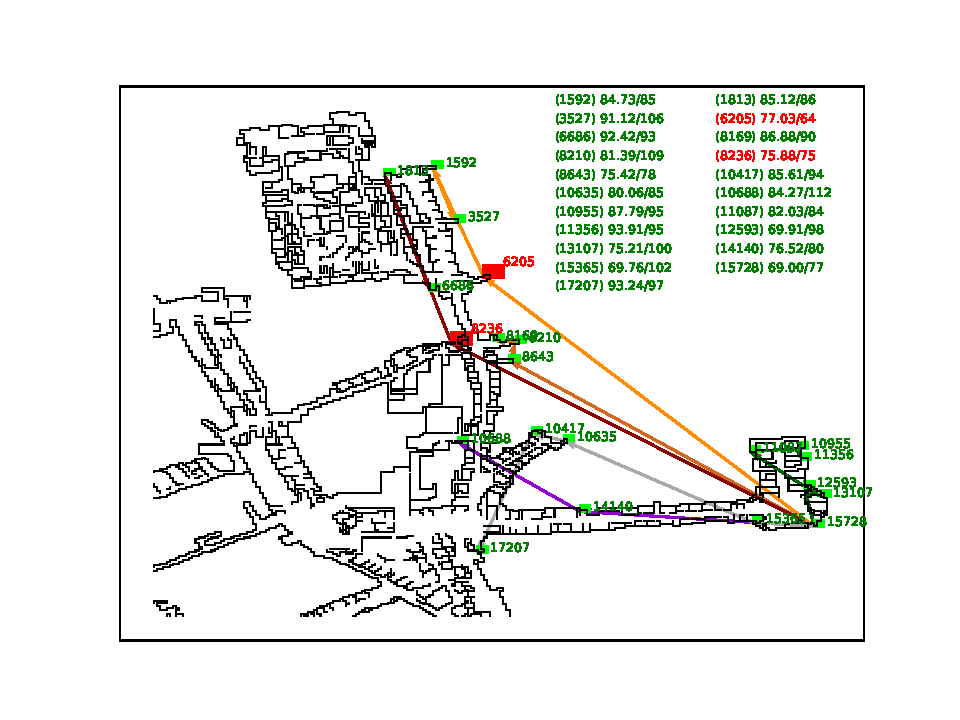
\includegraphics[width=8cm,trim=100 50 100 50]{fig/64min_6team_lim30min.pdf}
  \caption{設置開始時刻 64 分,設置チーム数 6,稼働時間上限 30 分での最
  適な止水板設置順序}
  \label{fig:64min_6team_lim30min_}
 \end{center}
\end{figure}

また,それぞれの場合の流入時間の合計を表 \ref{tb:ex2} に示す.

\begin{table}[htpb]
  \begin{center}
    \caption{実験 2 の結果}
    \begin{tabular}{cccc}\hline
     設置開始時刻(分) & 設置チーム数 & 稼働時間の上限(分) & 流入時間の合
		 計 (分) \\
     \hline
     43 & 6 & 30 & 0.00 \\
     57 & 6 & 30 & 6.03 \\
     64 & 6 & 30 & 13.91 \\
     \hline
      \end{tabular}
      \label{tb:ex2}
    \end{center}
\end{table}

\subsubsection{考察}

設置開始時刻が最も早い $43$ 分の場合,各設置チームが稼働時間の上限 $30$分
を守りつつ越水する全ての出入り口に止水板を設置することができ,かつ雨水の
流入を防ぐことができることがわかった.一方,設置開始時刻が遅くなるにつれ
流入時間の合計は長くなり,設置開始時刻が $64$ 分の場合には,流入時間の合
計が $13.91$ 分となることがわかった.また図
\ref{fig:43min_6team_lim30min_}, \ref{fig:57min_6team_lim30min_},
\ref{fig:64min_6team_lim30min_} からわかるように,水の流入する出入り口
(図中の赤い四角形の部分に相当)は設置開始時刻が $57$ 分の場合 $1$ 箇所,
$64$ 分の場合$2$ 箇所であることがわかる.

これらの結果は,(当然ではあるが,)できるだけ早く止水板の設置を開始すべ
きであるということを強く示唆している.また,本手法を用いることによって,
設置チームの最適な移動経路を算出ことができるため,得られた経路を非常時の
行動マニュアル等に生かすことができるものと考えられる.

\subsection{実験 3: 設置チーム数と流入時間の合計の関係}

稼働時間に上限がない場合,設置チーム数が少なくとも全ての出入り口に止水板
を設置することができるが,流入時間の合計は大きくなるはずである.本節での
では,この関係を定量的に評価するために,以下の条件で計算を行う:
%
\begin{itemize}
 \item 止水板設置開始時刻: 43, 57, 64 分
 \item 設置チーム数: 2, 3, 4, 5, 6 チーム
 \item 設置チームの稼働時間の上限: なし
\end{itemize}

\subsubsection{実験結果}

止水板設置開始時刻と設置チーム数の変化に伴って,流入時間の合計がどのよう
に変化するかをまとめたものが表 \ref{tb:ex3} である.

\begin{table}[htpb]
 \begin{center}
  \caption{設置チーム数・止水板設置開始時刻と流入時間の合計の関係}
  \begin{tabular}{c|ccc}
   \hline
   \backslashbox{設置チーム数}{止水板設置開始時刻} & 43 & 57 & 64 \\
   \hline
   6 & 0.00  & 6.03   & 13.91 \\
   5 & 0.00  & 6.03   & 13.91 \\
   4 & 0.00  & 6.03   & 24.21 \\
   3 & 0.00  & 34.73  & 138.82 \\
   2 & 66.76 & 203.70 & 288.33 \\
   \hline
  \end{tabular}
  \label{tb:ex3}
 \end{center}
\end{table}

また,止水板設置開始時刻が $64$ 分のとき,設置チーム数別に最適な移動経路,
すなわち最適な止水板の設置順序がどのように変化するかを図
\ref{fig:64min_2team_nolim_} から図 \ref{fig:64min_6team_nolim_} に示す.

\newpage

\begin{figure}[htpb]
 \begin{center}
  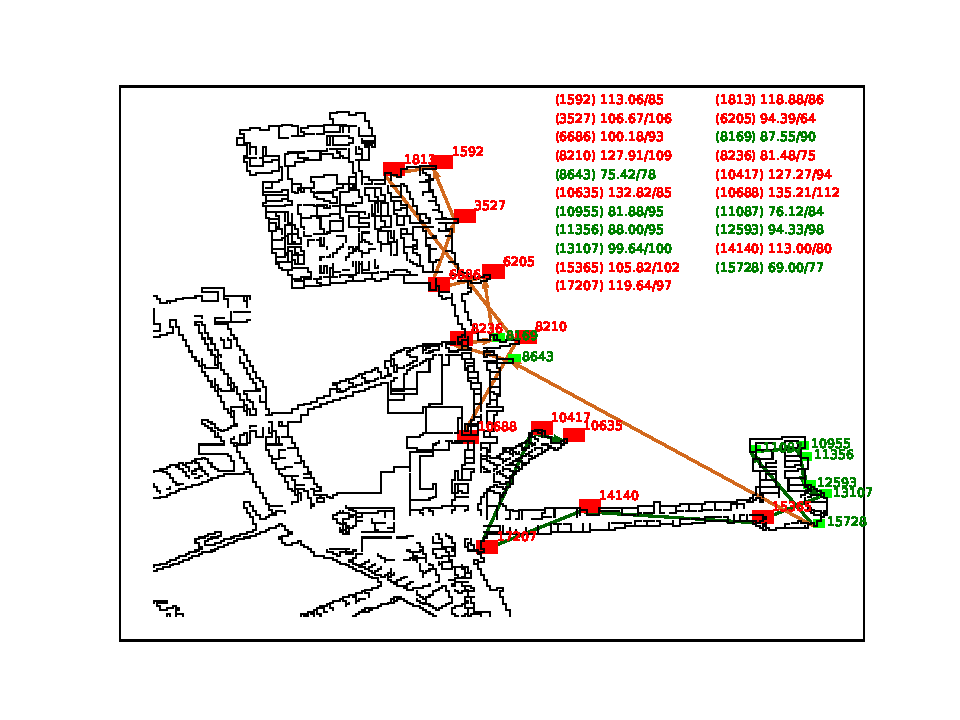
\includegraphics[width=8cm,trim=100 50 100 50]{fig/64min_2team_nolim.pdf}
  \caption{設置開始時刻 64 分,設置チーム数 2,稼働時間上限なしでの最
  適な止水板設置順序}
  \label{fig:64min_2team_nolim_}
 \end{center}
\end{figure}

\begin{figure}[htpb]
 \begin{center}
  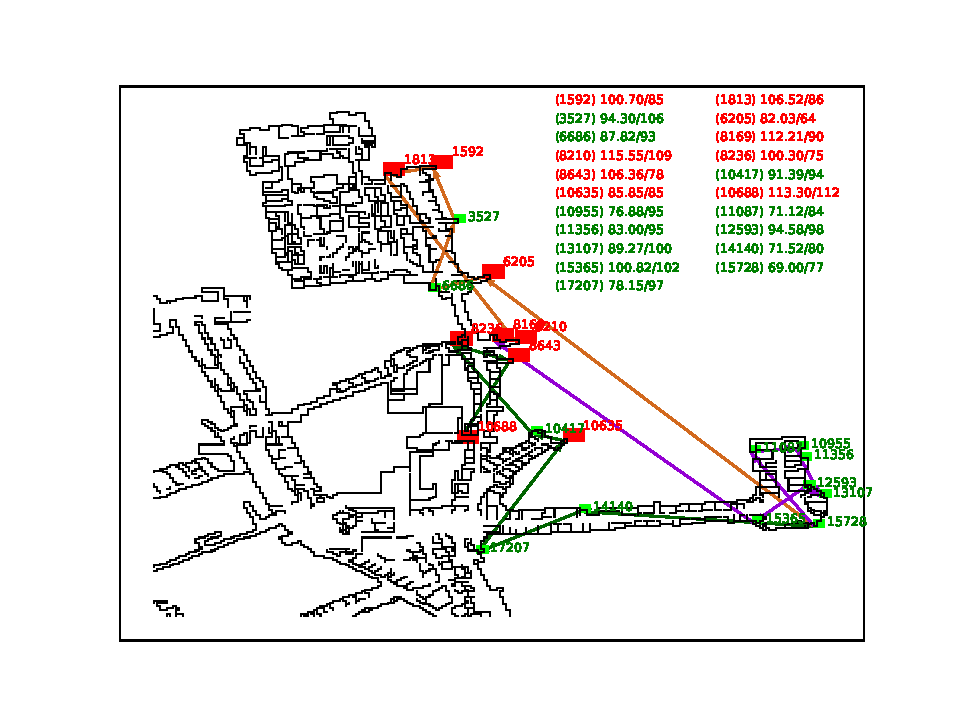
\includegraphics[width=8cm,trim=100 50 100 50]{fig/64min_3team_nolim.pdf}
  \caption{設置開始時刻 64 分,設置チーム数 3,稼働時間上限なしでの最
  適な止水板設置順序}
  \label{fig:64min_3team_nolim_}
 \end{center}
\end{figure}

\begin{figure}[htpb]
 \begin{center}
  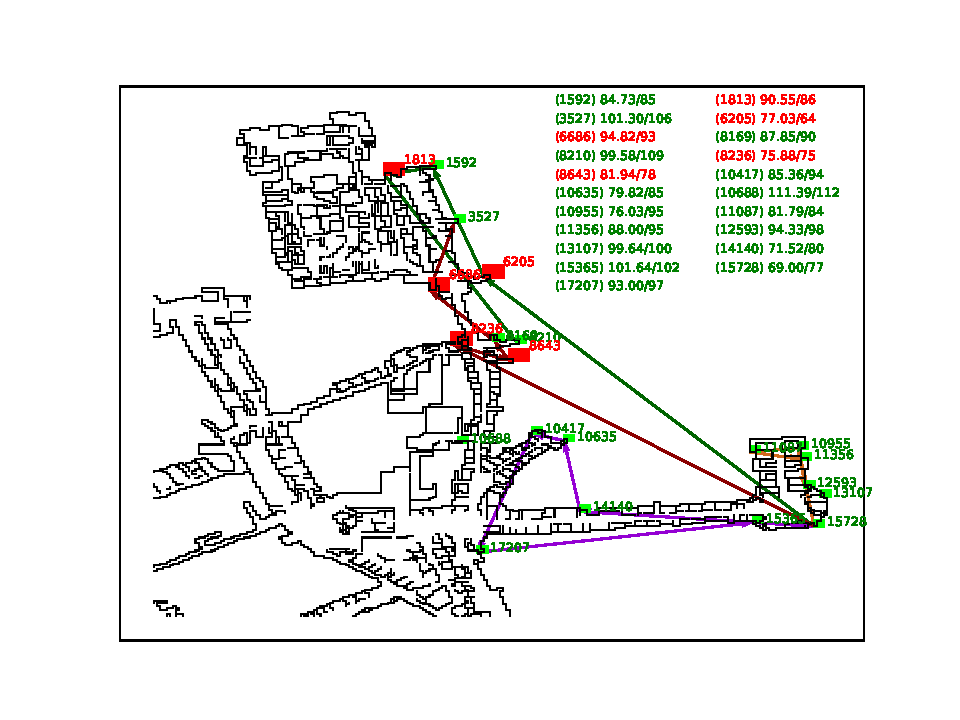
\includegraphics[width=8cm,trim=100 50 100 50]{fig/64min_4team_nolim.pdf}
  \caption{設置開始時刻 64 分,設置チーム数 4,稼働時間上限なしでの最
  適な止水板設置順序}
  \label{fig:64min_4team_nolim_}
 \end{center}
\end{figure}

\begin{figure}[htpb]
 \begin{center}
  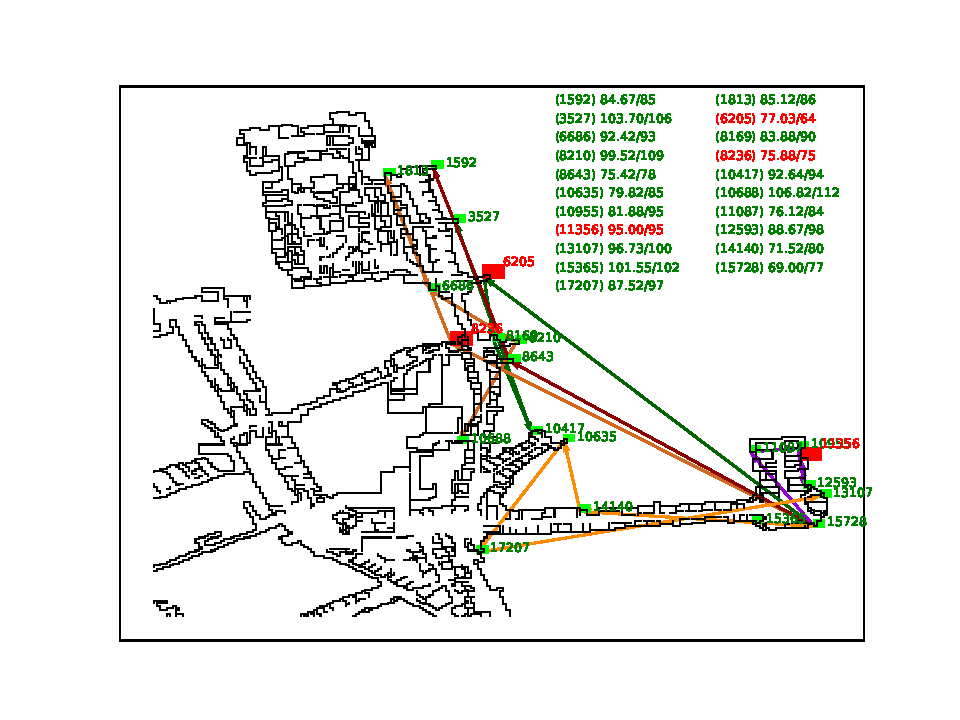
\includegraphics[width=8cm,trim=100 50 100 50]{fig/64min_5team_nolim.pdf}
  \caption{設置開始時刻 64 分,設置チーム数 5,稼働時間上限なしでの最
  適な止水板設置順序}
  \label{fig:64min_5team_nolim_}
 \end{center}
\end{figure}

\begin{figure}[htpb]
 \begin{center}
  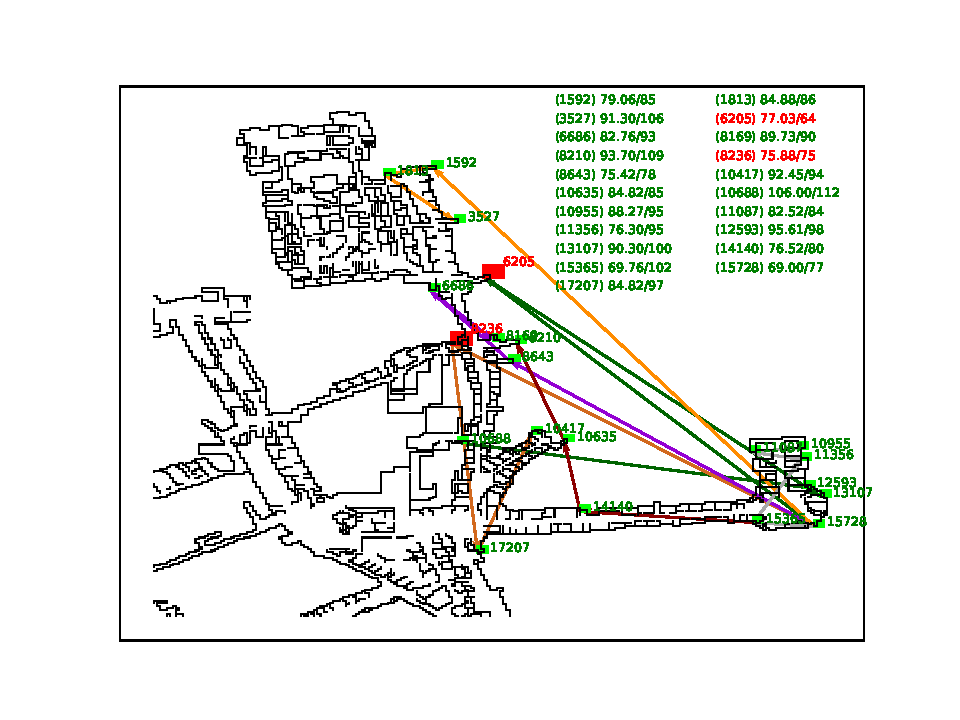
\includegraphics[width=8cm,trim=100 50 100 50]{fig/64min_6team_nolim.pdf}
  \caption{設置開始時刻 64 分,設置チーム数 6,稼働時間上限なしでの最
  適な止水板設置順序}
  \label{fig:64min_6team_nolim_}
 \end{center}
\end{figure}

\subsubsection{考察}

表 \ref{tb:ex3} からわかるように,いずれの設置開始時刻の場合も,設置チー
ム数が少なくなるにつれて,流入時間の合計が急激に増加する.すなわち,防災・
減災の観点からは,一定以上の設置チーム数を確保しておくことが必須である.

しかしながら,例えば夜間などのことを想定すると,設置チーム数が潤沢に準備
できない状況も想定される.そのような場合には,本計算で得られた最適な設置
順序を用いることによって,被害を最小限に食い止めることができるであろう.

%%%%%%%%%%%%%%%%%%%%%%%%%%%%%%%%%%%%%%%%%%%%%%%%%%%%%%%%%%%%%%%%%%%%%%
\if 1

この条件を基礎に実験を行う.実験条件の組み合わせは表 \ref{実験ケース1},,
表 \ref{実験ケース2},表 \ref{実験ケース3}に示す.\\

\begin{table}[H]
  \begin{center}
    \caption{実験 1 の条件}
    \scalebox{0.8}{
    \begin{tabular}{l|ccc}\hline
      \backslashbox{実験番号}{条件} & 止水板設置開始時刻(分) & 設置チーム数 & 各設置チームの稼動時間の制限(分)\\\hline
      実験 1$-$1 & 64 & 2$~$6 & 30 \\ 
      %実験 1$-$2 & 64 & 5 & 30 \\
      %実験 1$-$3 & 64 & 4 & 30 \\
      実験 1$-$2 & 64 & 2$~$6 & $-$ \\
      %実験 1$-$5 & 64 & 5 & $-$ \\
      %実験 1$-$6 & 64 & 4 & $-$ \\
      実験 1$-$3 & 57 & 2$~$6 & 30 \\
      %実験 1$-$8 & 57 & 5 & 30 \\
      %実験 1$-$9 & 57 & 4 & 30 \\
      実験 1$-$4 & 57 & 2$~$6 & $-$ \\
      %実験 1$-$11 & 57 & 5 & $-$ \\
      %実験 1$-$12 & 57 & 4 & $-$ \\
      実験 1$-$5 & 43 & 2$~$6 & 30 \\
      %実験 1$-$14 & 43 & 5 & 30 \\
      %実験 1$-$15 & 43 & 4 & 30 \\
      実験 1$-$6 & 43 & 2$~$6 & $-$ \\\hline
      %実験 1$-$17 & 43 & 5 & $-$ \\
      %実験 1$-$18 & 43 & 4 & $-$ \\\hline
      \end{tabular} }
      \label{実験ケース1}
    \end{center}
\end{table}

\begin{table}[H]
  \begin{center}
    \caption{実験 2 の条件}
     \scalebox{0.8}{
    \begin{tabular}{l|ccc}\hline
    \backslashbox{実験番号}{条件} & 設置チーム数 & 各設置チームの稼働時間の制限(分)\\\hline
    実験 2 & 2$~$6 & 40$~$60\\\hline
    %% 実験 2$-$2 & 57 & 2$~$6 & 40$~$60\\
    %% 実験 2$-$3 & 43 & 2$~$6 & 40$~$60\\\hline
    \end{tabular} }
    \label{実験ケース2}
  \end{center}
\end{table}
\begin{table}[H]
  \begin{center}
    \caption{実験 3 の条件}
     \scalebox{0.7}{
    \begin{tabular}{l|cccc}\hline
    \backslashbox{実験番号}{条件} & 止水板設置開始時刻(分) & 設置チーム数 & 各設置チームの稼働時間の制限(分) & 指定する設置経路\\\hline
    %実験 3$-$1 & 64 & 6 & 30 & 実験 1$-$1\\
    %実験 3$-$2 & 64 & 4$~$6 & $-$ & 実験 1$-$2\\
    実験 3$-$1 & 57 & 6 & 30 & 実験 1$-$1\\
    実験 3$-$2 & 57 & 4$~$6 & $-$ & 実験 1$-$2\\
    実験 3$-$3 & 43 & 6 & 30 & 実験 1$-$1\\
    実験 3$-$4 & 43 & 4$~$6 & $-$ & 実験 1$-$2\\\hline
    \end{tabular} }
    \label{実験ケース3}
  \end{center}
\end{table}


馬谷の研究では梅田地下街全域を対象として研究を行っていたが,梅田地下街は複数の管理主体が存在し,それぞれの地区に管理施設を持つ.本研究ではホワイティうめだの管理施設に限定して実験を行っていく.図 \ref{whity} はホワイティうめだの 1 時間当たりの降雨量 120mm,排水用ポンプが稼働している場合に流入する可能性のある出入り口 21 箇所を示している.

\begin{figure}[H]
\begin{center}
  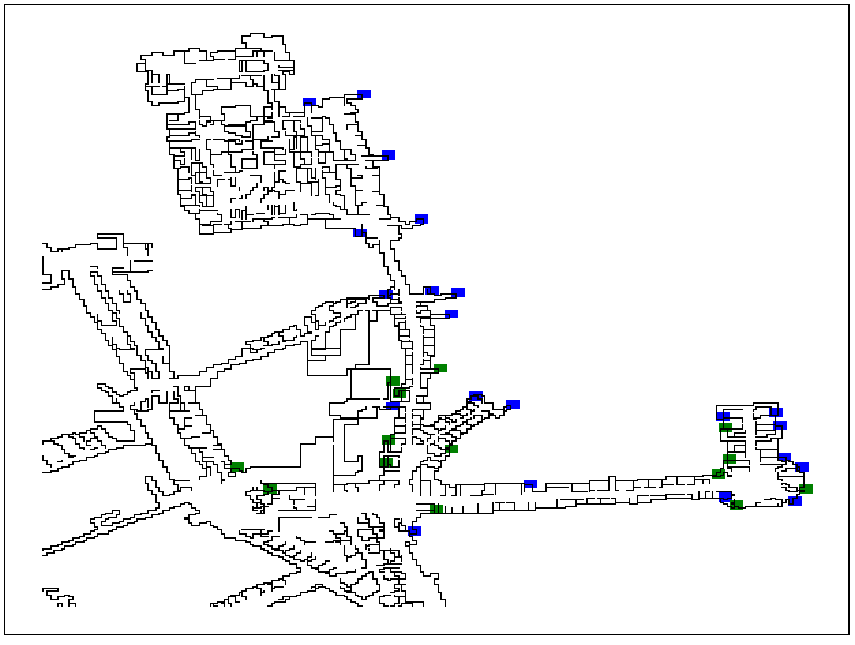
\includegraphics[width=10cm,bb=0.0 0.0 410.4 309.6, clip]{whity_map.pdf}
  \caption{ホワイティうめだ出入口}
  \label{whity}
  \end{center}
\end{figure}

    
    
\subsection{実験 1}
本節では止水板設置開始時刻を $57$, $43$ 分に変化させ,それぞれ設置チーム 2$~$6 チームの場合の実験を行った.

\subsubsection{実験 1$-$1}
\begin{itemize}
\item 止水板設置開始時刻 64 分
\item 設置チームの稼働時間 30 分


\begin{itemize}
\item 6 チームの場合
\end{itemize}

\begin{figure}[H]
\begin{center}
  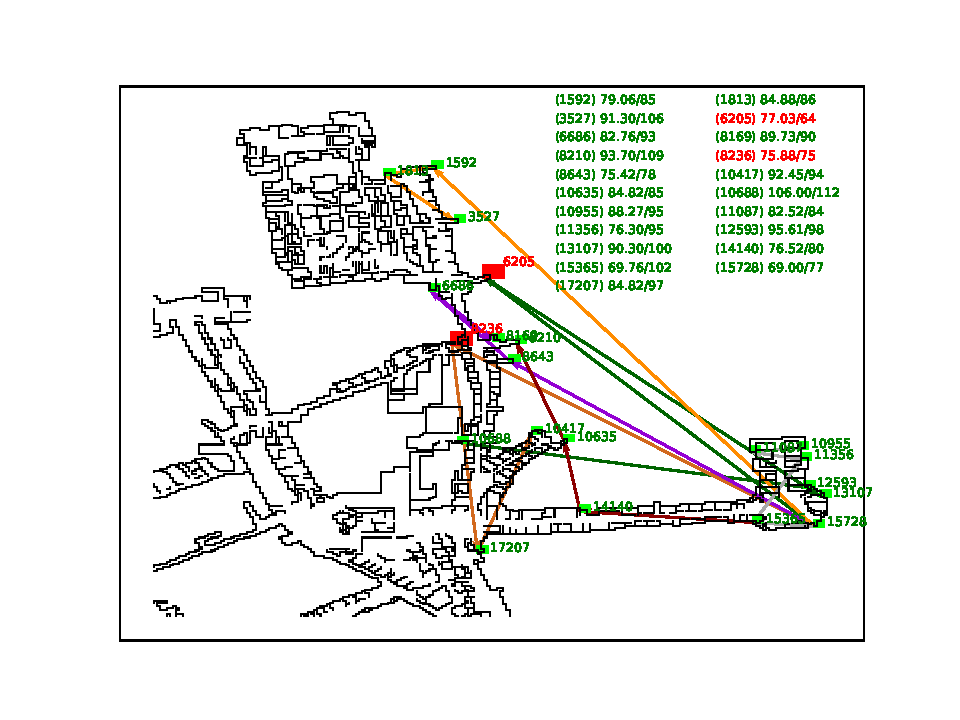
\includegraphics[width=10cm,clip]{st64_t6_no30.pdf}
  \caption{6 チームの場合}
  \label{fig:st64_t6_no30}
  \end{center}
\end{figure}


%% \begin{table}[H]
%%   \begin{center}
%%     \caption{設置順序}
%%     \begin{tabular}{l|cccccc}\hline
%%      \backslashbox {レイヤの数}{設置チーム名} & a & b & c & d & e & f \\\hline
%%       0 & 15728 & 15728 & 15728 & 15728 & 15728 & 15728 \\
%%       1 & 12593 & 8643 & 15728 & 8236 & 6205 & 15365 \\
%%       2 & 13107 & 8210 & 14140 & 1813 & 1592 & 10635 \\
%%       3 & 11087 & 8169 & 10688 & 6686 & 3527 & 10417 \\
%%       4 & 10955 & $-$ & $-$ & $-$ & $-$ & 17207 \\
%%       5 & 11356 & $-$ & $-$ & $-$ & $-$ & $-$ \\\hline
%%     \end{tabular}
%%     \label{fig:実験1_1_1}
%%   \end{center}
%% \end{table}

%% \begin{table}[H]
%%   \begin{center}
%%     \caption{$6$ チームの場合の流入箇所}
%%     \begin{tabular}{lrrr}\hline
%%       設置チーム名 & レイヤ数 & 出入り口メッシュ番号 & 流入時間(分)\\\hline
%%       d & 1 & 8236 & 0.88 \\
%%       e & 1 & 6205 & 13.03\\\hline
%%     \end{tabular}
%%     \label{fig:実験1_1_2}
%%   \end{center}
%% \end{table}


\begin{itemize}
\item $5$ チームの場合 \\
$5$ チームの条件で計算を行うと,$1$ 時間($=3600$ 秒)経過した時点で暫定解は得られなかった.そこで計算を $24$ 時間($=86400$ 秒)行ったが,暫定解を得ることはできなかった.
\end{itemize}

\begin{itemize}
\item $4$ チームの場合 \\
$4$ チームの条件で計算を行うと実行不可能となった.つまり,$4$ チームでは各チームの稼働時間 $30$ 分以内に全ての止水板を設置することはできない.\\
$4$ チームの条件で実行不可能という結果が出たということは,さらに条件が厳しくなる $3$ チームと $2$ チームも同様に実行不可能であることが推測できる.
\end{itemize}

\begin{table}[H]
  \begin{center}
    \caption{実験 $1-1$ の計算結果}
    \scalebox{0.9}{
    \begin{tabular}{l|ccccc}\hline
     \backslashbox{チーム数}{計算結果} & 計算時間(s) & 制約数 & 変数の数 & GAP(\%) & 流入時間の合計(分)\\\hline
      6 & 1540 & 16866 & 47832 & 0.00 & 13.91 \\
      5 & 86400 & 14055 & 39867 & $-$ & $-$\\
      4 & 3479 & 27984 & 79674 & $-$ & $-$\\\hline
      %3 & 1 & 8433 & 23937 & $-$ & $-$\\
      %2 & 3600 & 13992 & 39858 & $-$ & $-$\\\hline
    \end{tabular} }
    \label{実験1_1_3}
  \end{center}
\end{table}
\end{itemize}


\subsubsection{実験 1$-$2}
\begin{itemize}
\item 止水板設置開始時刻 64 分
\item 設置チームの稼働時間上限なし


\begin{itemize}
\item 6 チームの場合
\end{itemize}

\begin{figure}[H]
\begin{center}
  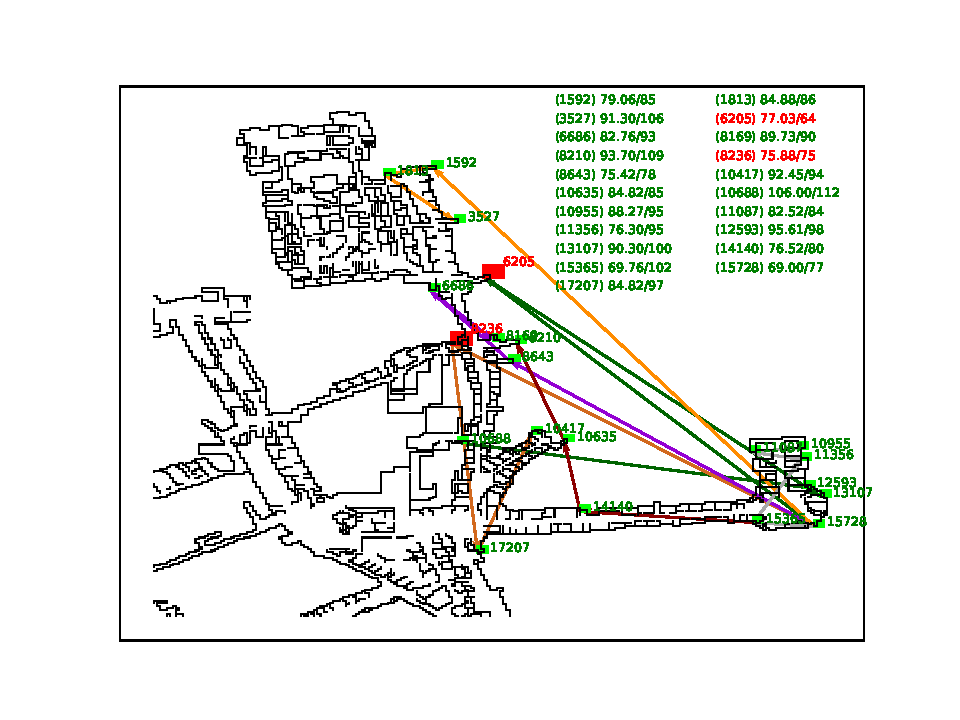
\includegraphics[width=10cm,clip]{st64_t6_no30.pdf}
  \caption{6 チームの場合}
  \label{fig:st64_t6_no30}
  \end{center}
\end{figure}

\begin{itemize}
\item 5 チームの場合
\end{itemize}

\begin{figure}[H]
\begin{center}
  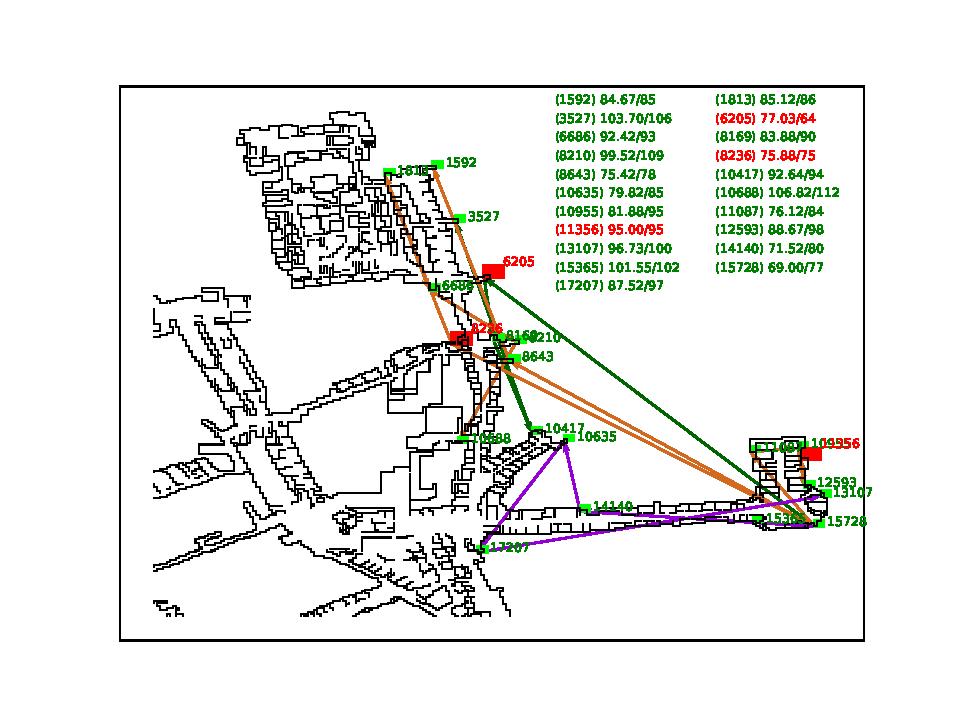
\includegraphics[width=10cm,clip]{st64_t5_no30.pdf}
  \caption{5 チームの場合}
  \label{fig:st64_t5_no30}
  \end{center}
\end{figure}

\begin{itemize}
\item 4 チームの場合
\end{itemize}

\begin{figure}[H]
\begin{center}
  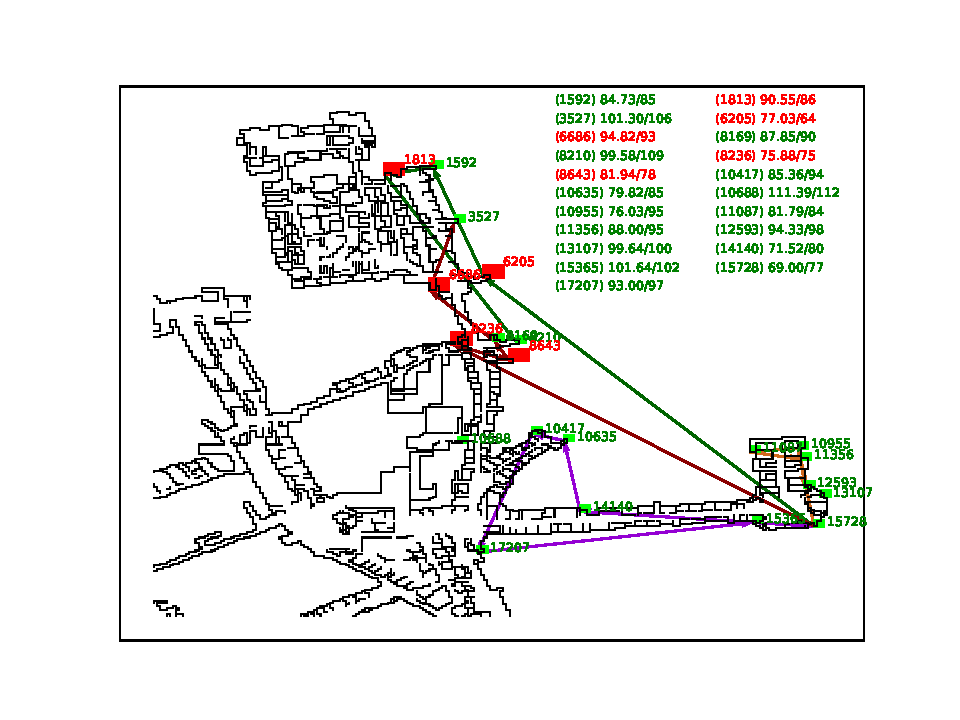
\includegraphics[width=10cm,clip]{st64_t4_no30.pdf}
  \caption{4 チームの場合}
  \label{fig:st64_t4_no30}
  \end{center}
\end{figure}

\begin{itemize}
\item 3 チームの場合
\end{itemize}

\begin{figure}[H]
\begin{center}
  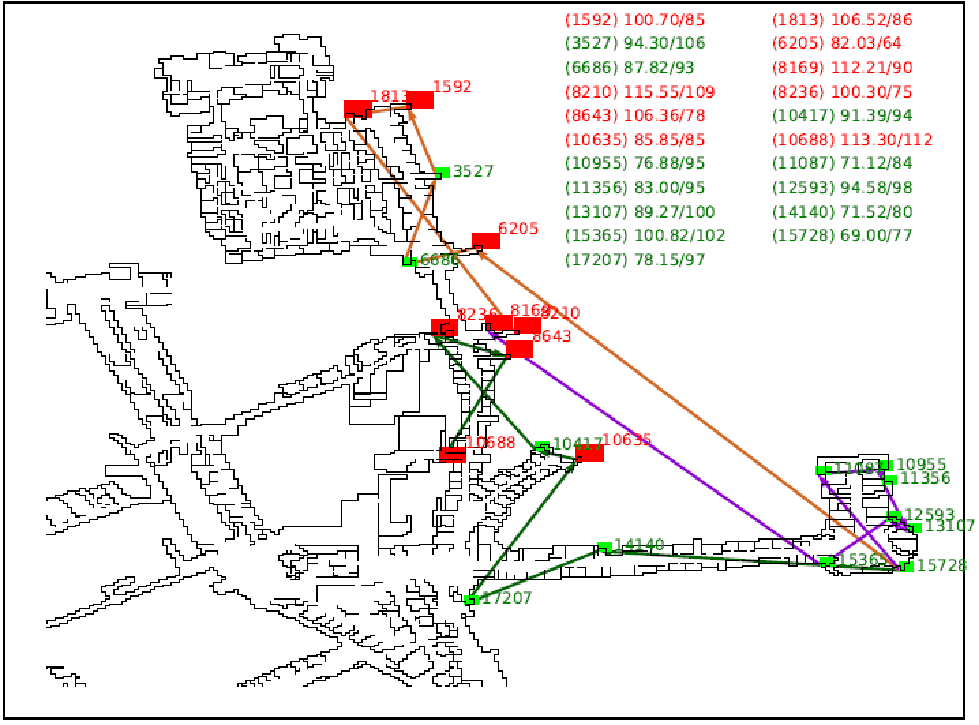
\includegraphics[width=10cm,clip]{st64_t3_no30.pdf}
  \caption{3 チームの場合}
  \label{fig:st64_t3_no30}
  \end{center}
\end{figure}

\begin{itemize}
\item 2 チームの場合
\end{itemize}

\begin{figure}[H]
\begin{center}
  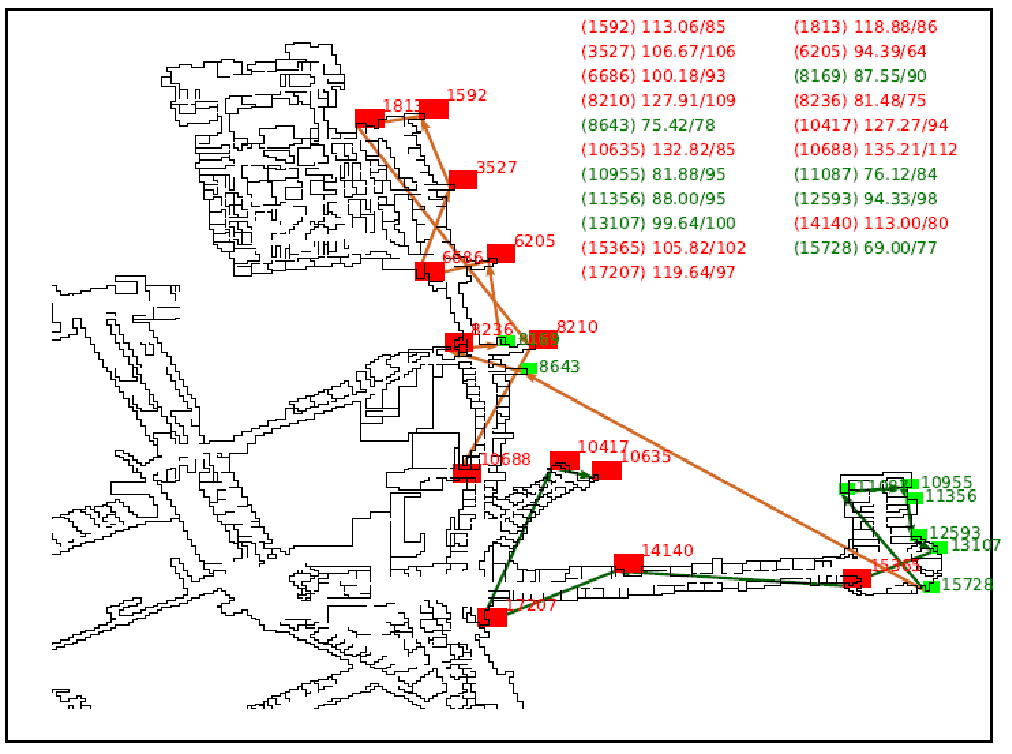
\includegraphics[width=10cm,clip]{st64_t2_no30.pdf}
  \caption{2 チームの場合}
  \label{fig:st64_t2_no30}
  \end{center}
\end{figure}

\begin{table}[H]
\begin{center}
\caption{実験 $1-2$ の計算結果}
\scalebox{0.9}{
\begin{tabular}{l|ccccc}\hline
\backslashbox{チーム数}{計算結果} & 計算時間(s) & 制約数 & 変数の数 & GAP(\%) & 流入時間の合計(分)\\\hline
6 & 587 & 16866 & 47826 & 0.00 & 13.91 \\
5 & 935 & 14055 & 29862 & 0.00 & 13.91\\
4 & 3600 & 11244 & 31898 & 46.18 & 24.21\\
3 & 3600 & 20988 & 59763 & 96.40 & 138.82\\
2 & 3600 & 13992 & 39856 & 98.27 & 288.33\\\hline
\end{tabular} }
\label{実験1_2_2}
\end{center}
\end{table}
\end{itemize}


\subsubsection{実験 1$-$3}
\begin{itemize}
\item 止水板設置開始時刻 57 分
\item 設置チームの稼働時間 30 分

\begin{itemize}
\item 6 チームの場合
\end{itemize}

\begin{figure}[H]
\begin{center}
  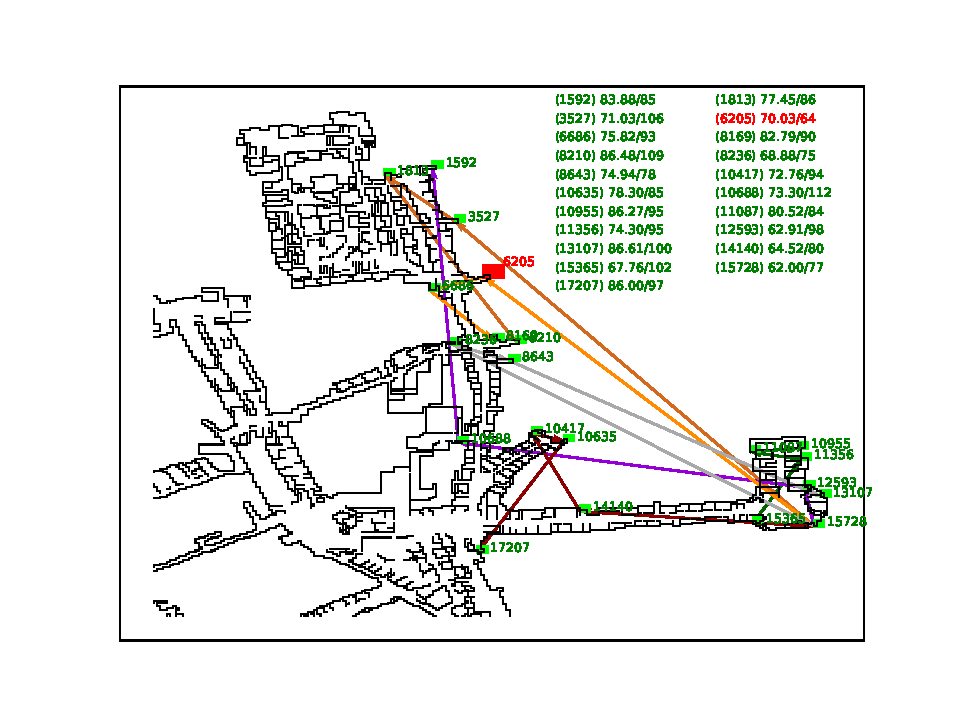
\includegraphics[width=10cm,clip]{st57_t6.pdf}
  \caption{6 チームの場合}
  \label{fig:st57_t6}
  \end{center}
\end{figure}

\begin{itemize}
\item $5$ チームの場合\\
$5$ チームの条件で計算を行うと,1 時間(=3600 秒)経過した時点で暫定解を得ることはできなかった.
\end{itemize}

\begin{itemize}
\item $4$ チームの場合\\
$4$ チームの条件で計算を行うと実行不可能となった.\\
この結果から,設置チーム $3$ チームと $2$ チームの場合も同様に実行不可能であることが想定される.
\end{itemize}

\begin{table}[H]
\begin{center}
\caption{計算結果}
\scalebox{0.9}{
\begin{tabular}{l|ccccc}\hline
\backslashbox{チーム数}{計算結果} & 計算時間(s) & 制約数 & 変数の数 & GAP(\%) & 流入時間の合計(分)\\\hline
6 & 402 & 16866 & 47832 & 0.00 & 6.03\\
5 & 3600 & 14055 & 39867 & $-$ & $-$\\
4 & 3600 & 27984 & 79674 & $-$ & $-$\\\hline
\end{tabular} }
\label{実験1_3_2}
\end{center}
\end{table}
\end{itemize}

\subsubsection{実験 1$-$4}
\begin{itemize}
\item 止水板設置開始時刻 57 分
\item 設置チームの稼働時間上限なし

\begin{itemize}
\item $6$ チームの場合
\end{itemize}

\begin{figure}[H]
\begin{center}
  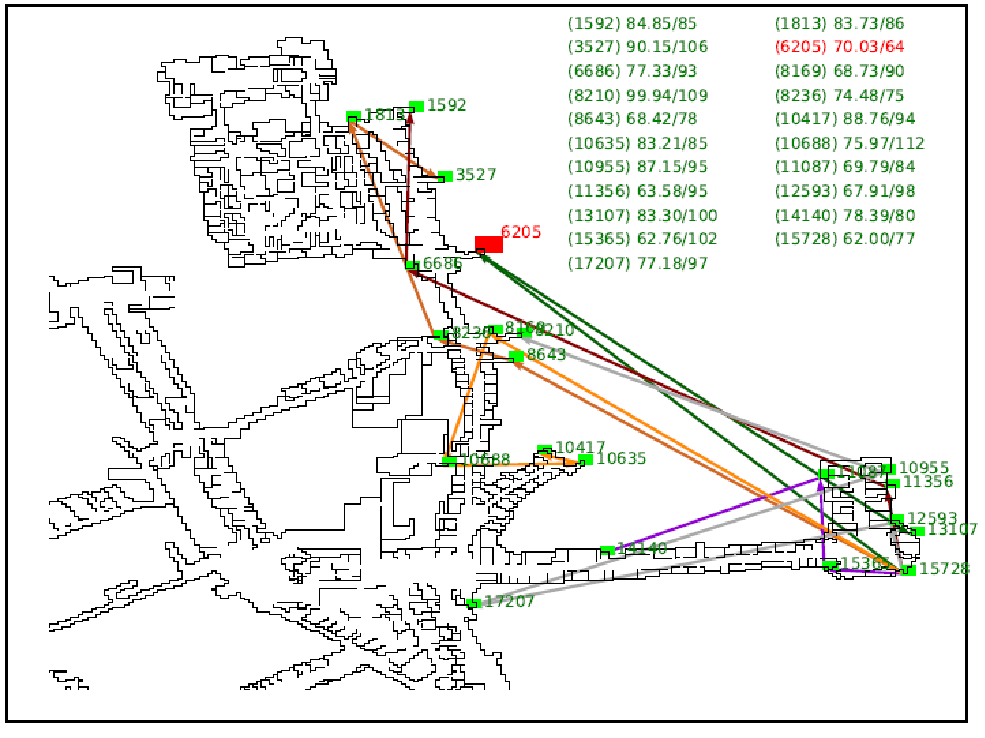
\includegraphics[width=10cm,clip]{st57_t6_no30.pdf}
  \caption{6 チームの場合}
  \label{fig:st57_t6_no30}
  \end{center}
\end{figure}

\begin{itemize}
\item $5$ チームの場合
\end{itemize}

\begin{figure}[H]
\begin{center}
  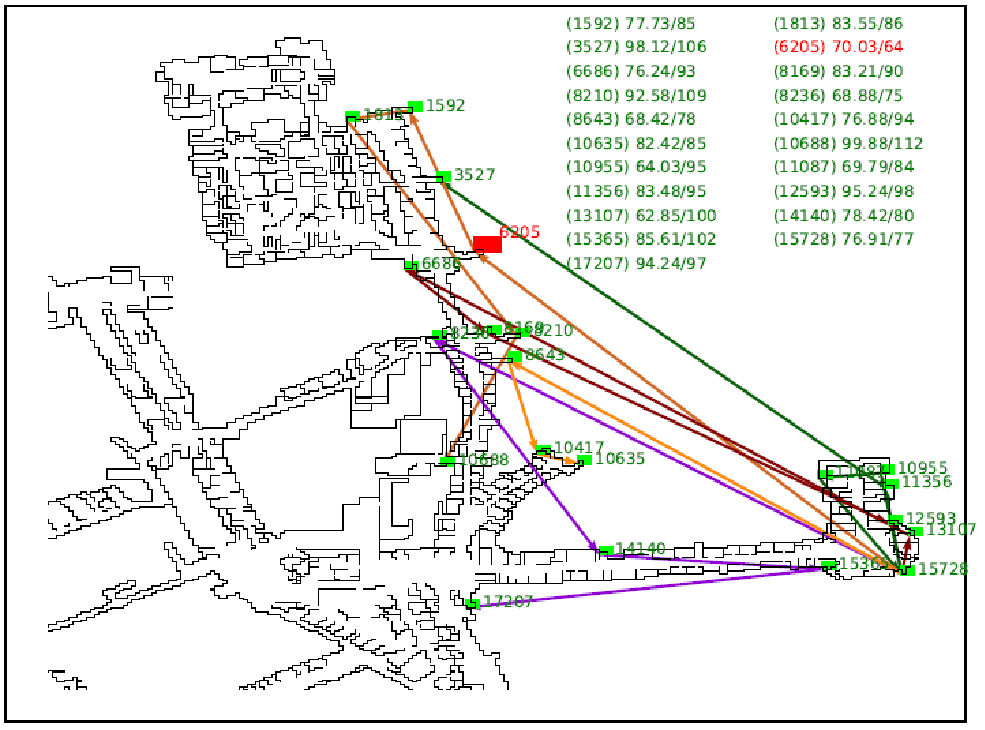
\includegraphics[width=10cm,clip]{st57_t5_no30.pdf}
  \caption{5 チームの場合}
  \label{fig:st57_t5_no30}
  \end{center}
\end{figure}

\begin{itemize}
\item $4$ チームの場合
\end{itemize}

\begin{figure}[H]
\begin{center}
  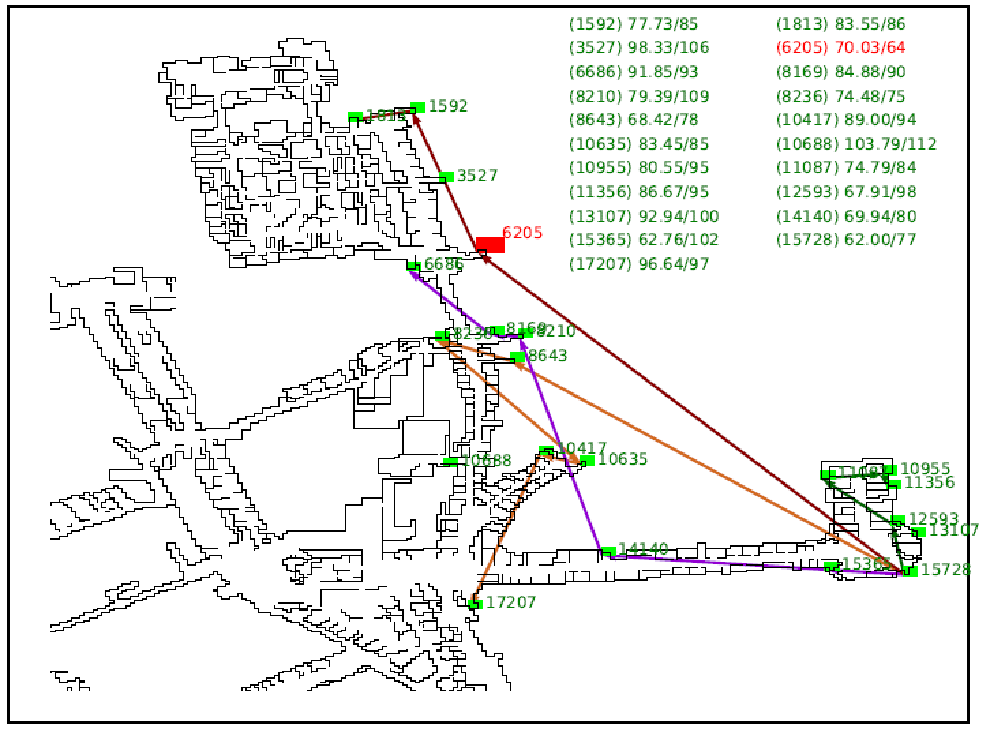
\includegraphics[width=10cm,clip]{st57_t4_no30.pdf}
  \caption{4 チームの場合}
  \label{fig:st57_t4_no30}
  \end{center}
\end{figure}

\begin{itemize}
\item $3$ チームの場合
\end{itemize}

\begin{figure}[H]
\begin{center}
  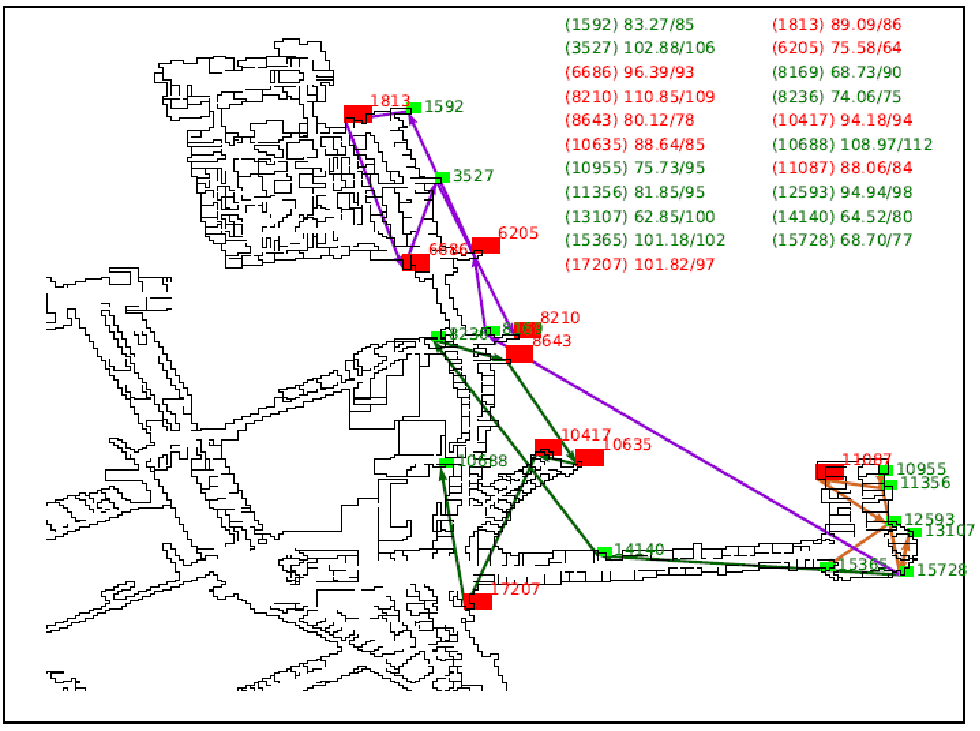
\includegraphics[width=10cm,clip]{st57_t3_no30.pdf}
  \caption{3 チームの場合}
  \label{fig:st57_t3_no30}
  \end{center}
\end{figure}



\begin{itemize}
\item $2$ チームの場合
\end{itemize}

\begin{figure}[H]
\begin{center}
  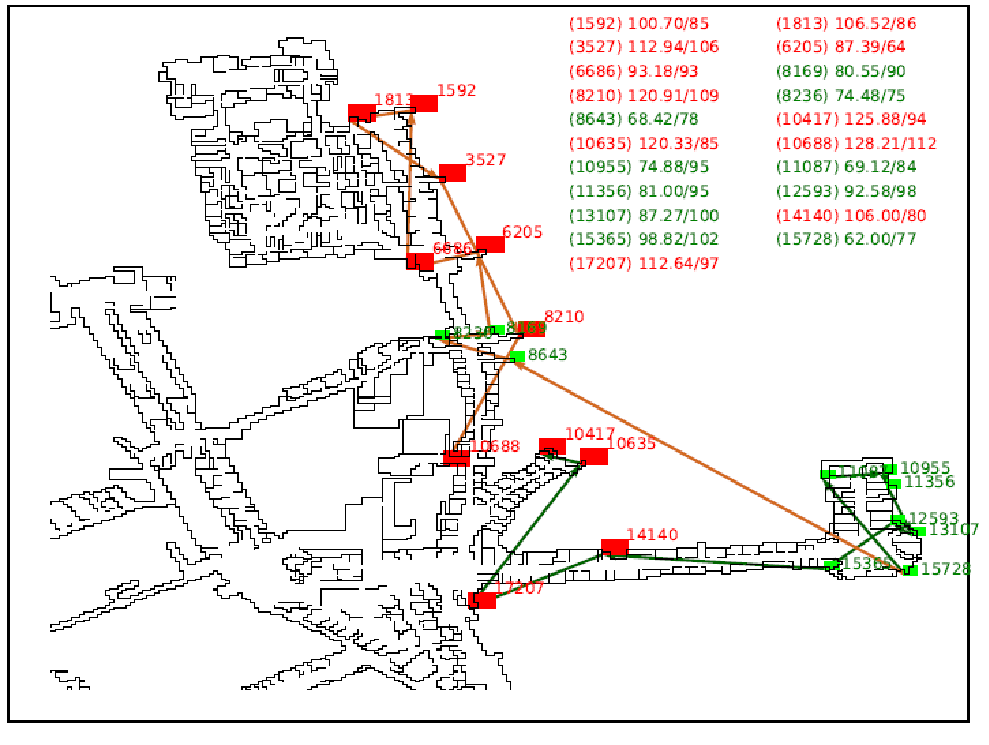
\includegraphics[width=10cm,clip]{st57_t2_no30.pdf}
  \caption{2 チームの場合}
  \label{fig:st57_t2_no30}
  \end{center}
\end{figure}




\begin{table}[H]
\begin{center}
\caption{計算結果}
\scalebox{0.9}{
\begin{tabular}{l|ccccc}\hline
\backslashbox{チーム数}{計算結果} & 計算時間(s) & 制約数 & 変数の数 & GAP(\%) & 流入時間の合計(分)\\\hline
6 & 59 & 16866 & 47826 & 0.00 & 6.03\\
5 & 85 & 14055 & 39862 & 0.00 & 6.03\\
4 & 426 & 11244 & 31898 & 0.00 & 6.03\\
3 & 3600 & 20988 & 59763 & 100 & 34.73\\
2 & 3600 & 13992 & 39856 & 100 & 203.70\\\hline
\end{tabular} }
\label{実験1_4_2}
\end{center}
\end{table}
\end{itemize}

\subsubsection{実験 1$-$5}
\begin{itemize}
\item 止水板設置開始時刻 43 分
\item 設置チームの稼働時間 30 分



\begin{itemize}
\item $6$ チームの場合\\
\end{itemize}

\begin{figure}[H]
\begin{center}
  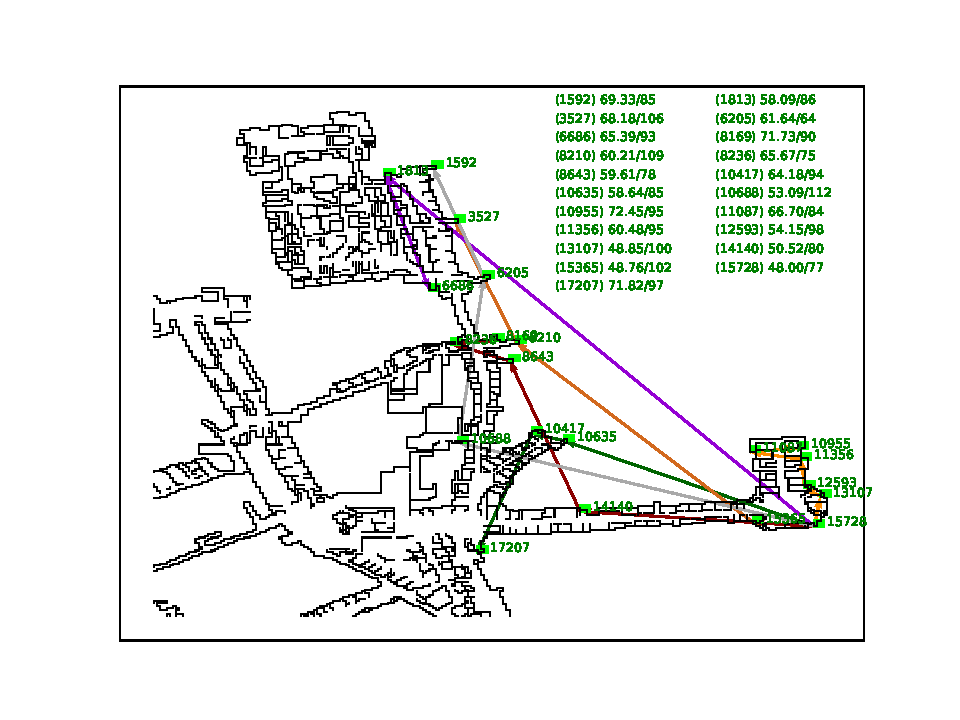
\includegraphics[width=10cm,clip]{st43_t6.pdf}
  \caption{6 チームの場合}
  \label{fig:st43_t6}
  \end{center}
\end{figure}


\begin{itemize}
\item $5$ チームの場合\\
$5$ チームの条件で計算を行うと,1 時間(=3600 秒)経過した時点で暫定解を得ることができなかった.
\end{itemize}

\begin{itemize}
\item 4 チームの場合\\
4 チームの条件で計算を行った結果,実行不可能となった.\\
この結果から 3 チームと 2 チームの場合も実行不可能であることが推測できる.
\end{itemize}

\begin{table}[H]
\begin{center}
\caption{計算結果}
\scalebox{0.9}{
\begin{tabular}{l|ccccc}\hline
\backslashbox{チーム数}{計算結果} & 計算時間(s) & 制約数 & 変数の数 & GAP(\%) & 流入時間の合計(分)\\\hline
6 & 31 & 16866 & 47832 & 0.00 & 0.00\\
5 & 3600 & 14055 & 39867 & $-$ & $-$\\
4 & 3600 & 27984 & 79674 & $-$ & $-$\\\hline
\end{tabular} }
\label{実験1_5_1}
\end{center}
\end{table}
\end{itemize}


\subsubsection{実験 1$-$6}
\begin{itemize}
\item 止水板設置開始時刻 43 分
\item 設置チームの稼働時間上限なし


\begin{itemize}
\item 6 チームの場合\\
\end{itemize}

\begin{figure}[H]
\begin{center}
  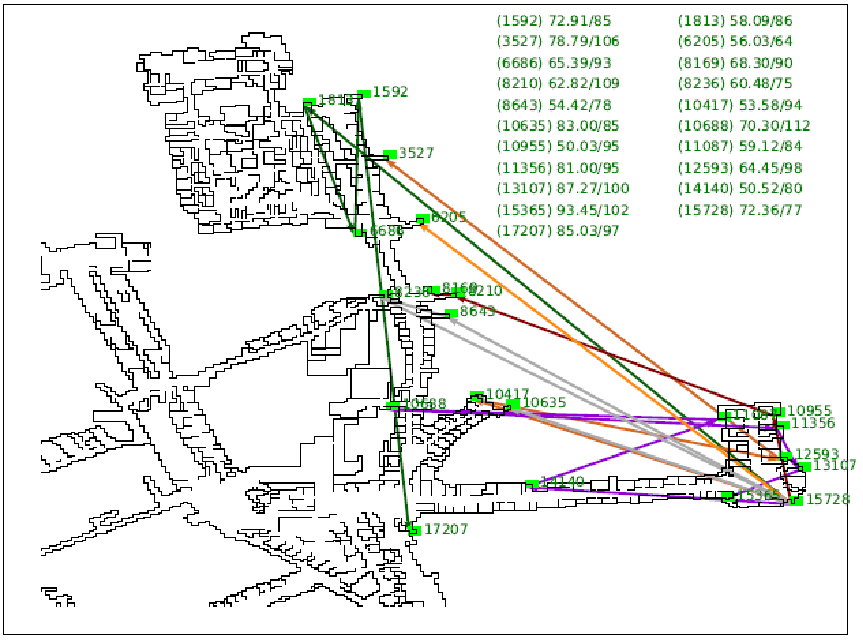
\includegraphics[width=10cm,clip]{st43_t6_no30.pdf}
  \caption{6 チームの場合}
  \label{fig:st43_t6_no30}
  \end{center}
\end{figure}

\begin{itemize}
\item $5$ チームの場合\\
\end{itemize}

\begin{figure}[H]
\begin{center}
  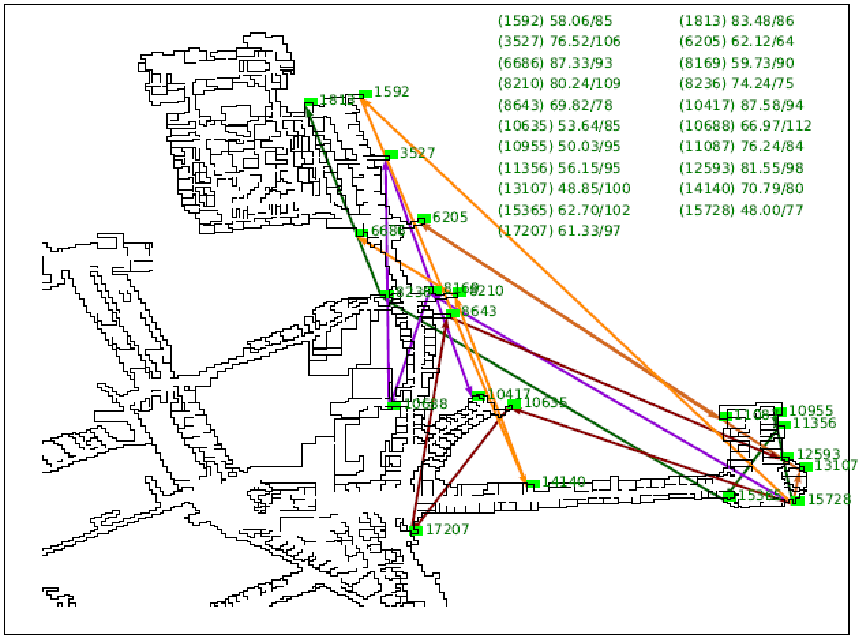
\includegraphics[width=10cm,clip]{st43_t5_no30.pdf}
  \caption{5 チームの場合}
  \label{fig:st43_t5_no30}
  \end{center}
\end{figure}


\begin{itemize}
\item $4$ チームの場合\\
\end{itemize}

\begin{figure}[H]
\begin{center}
  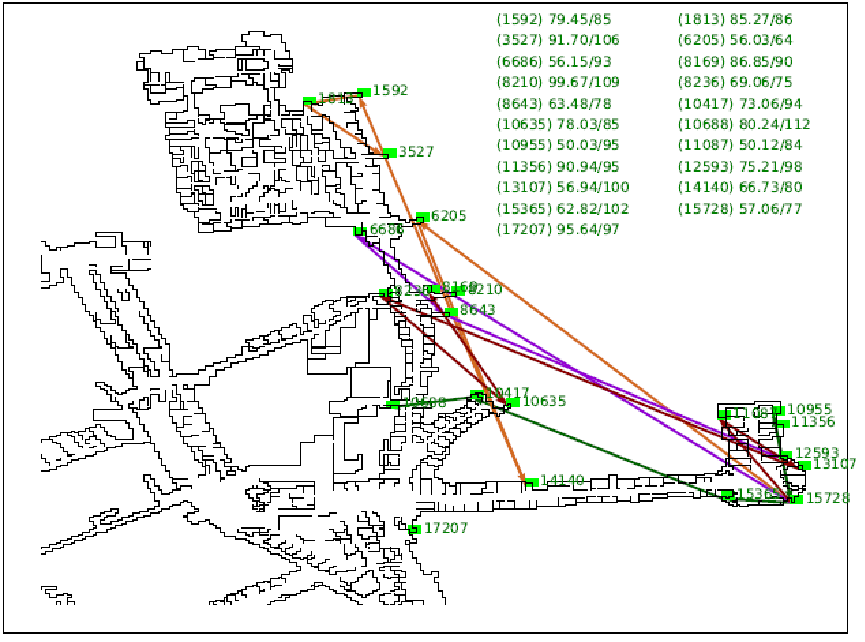
\includegraphics[width=10cm,clip]{st43_t4_no30.pdf}
  \caption{4 チームの場合}
  \label{fig:st43_t4_no30}
  \end{center}
\end{figure}

\begin{itemize}
\item $3$ チームの場合
\end{itemize}

\begin{figure}[H]
\begin{center}
  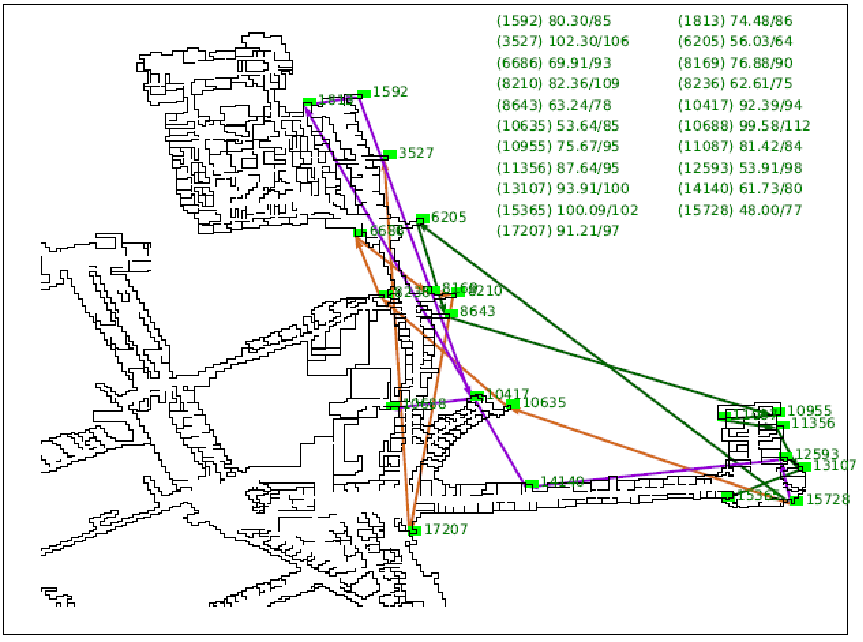
\includegraphics[width=10cm,clip]{st43_t3_no30.pdf}
  \caption{3 チームの場合}
  \label{fig:st43_t3_no30}
  \end{center}
\end{figure}



\begin{itemize}
\item  $2$ チームの場合
\end{itemize}

\begin{figure}[H]
\begin{center}
  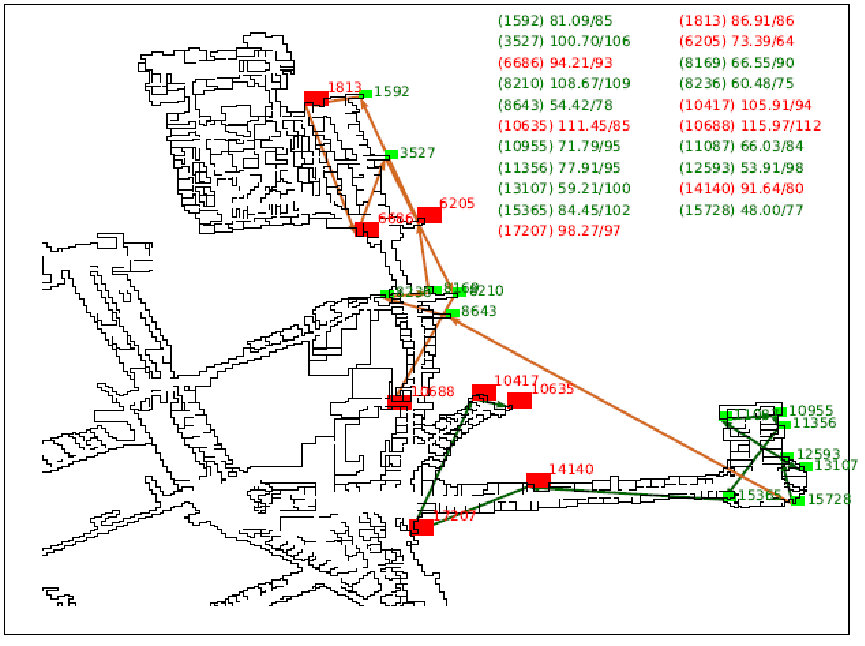
\includegraphics[width=10cm,clip]{st43_t2_no30.pdf}
  \caption{2 チームの場合}
  \label{fig:st43_t2_no30}
  \end{center}
\end{figure}

\begin{table}[H]
\begin{center}
\caption{計算結果}
\scalebox{0.9}{
\begin{tabular}{l|ccccc}\hline
\backslashbox{チーム数}{計算結果} & 計算時間(s) & 制約数 & 変数の数 & GAP(\%) & 流入時間の合計(分)\\\hline
6 & 3.0 & 16866 & 47826 & 0.00 & 0.00\\
5 & 402 & 14055 & 39862 & 0.00 & 0.00\\
4 &  4 & 11244 & 31898 & 0.00 & 0.00\\
3 & 3186  & 20988 & 59763 & 0.00 & 0.00\\
2 & 3600 & 13992 & 39856 & 100 & 66.76\\\hline
\end{tabular} }
\label{実験1_6_1}
\end{center}
\end{table}
\end{itemize}

表\ref{30分制限あり},表\ref{30分制限なし}は実験 1 の結果をまとめた表である.

\begin{table}[H]
\begin{center}
\caption{稼働時間 30 分の流入時間}
\begin{tabular}{l|ccc}\hline
\backslashbox{($A$)}{($B$)} & 64 & 57 & 43\\\hline
6 & 13.91 & 6.0 & 0.0\\     
5 & 暫定解なし & 暫定解なし & 暫定解なし\\
4 & 実行不可能 & 実行不可能 & 実行不可能\\
3 & 実行不可能 & 実行不可能 & 実行不可能\\
2 & 実行不可能 & 実行不可能 & 実行不可能\\\hline
\end{tabular}
\label{30分制限あり}
\end{center}
\end{table}

\begin{table}[H]
\begin{center}
\caption{稼働時間上限なしの流入時間}
\begin{tabular}{l|ccc}\hline
\backslashbox{($A$)}{($B$)} & 64 & 57 & 43\\\hline
6 & 13.91 & 6.03 & 0.00\\
5 & 13.91 & 6.03 & 0.00\\
4 & 24.21 & 6.03 & 0.00\\
3 & 138.82 & 34.73 & 0.00\\
2 & 288.33 & 203.70 & 66.76\\\hline
\end{tabular}
\label{30分制限なし}
\end{center}
\end{table}

\hspace{4.0cm}($A$) : 設置チーム数\\
\hspace{4.4cm}($B$) : 止水板設置開始時刻(分)

\subsubsection{考察}
実験 $1$ の結果より設置チームの稼働時間 30 分に制限すると,4 チーム以下では全ての止水板設置開始時刻において 30 分以内に止水板を設置することは不可能であることが分かる.5 チームの場合では計算開始して 24 時間経過した時点で暫定解を得ることができなかった.つまり,設置可能か不可能か判断することができなかった.6 チームの場合は全ての止水板設置開始時刻において設置可能であった.このことから,設置チームの稼働時間を 30 分に制限する場合は少なくとも 6 チームは必要であることが分かる.

止水板設置チームの制限時間の上限なしの場合では $2~6$ チームにおいて全ての出入り口に止水板を設置することが可能であった.止水板設置開始時刻 64,57 分では 3 チームになると流入時間が急激に長くなり,43 分では 3 チームまで流入はしていなかったが 2 チームになると 66 分になる.設置チームの制限時間の上限をなしにするとチーム数が少なくなってもすべての止水板を設置することはできるが,一定のチーム数まで少なくなると流入時間は急激に長くなる.

\subsection{実験 2}
本節では止水板設置チームの稼働時間を $40~60$ 分に変化させて止水板設置が可能であるかを検討した.

\begin{table}[H]
\begin{center}
\caption{実験 $2$ : 計算結果}
\begin{tabular}{l|cccc}\hline
\backslashbox{チーム数}{稼働時間} & 30 & 40 & 50 & 60\\\hline
6 & 可能 & 可能 & 可能 & 可能\\
5 & 暫定解なし & 可能 & 可能 & 可能\\
4 & 不可能 & 可能 & 可能 & 可能\\
3 & 不可能 & 不可能 & 暫定解なし & 不可能\\
2 & 不可能 & 不可能 & 不可能 & 不可能\\\hline
\end{tabular}
\label{64分制限時間変化}
\end{center}
\end{table}


%% \subsubsection{実験 $2-2$}
%% \begin{itemize}
%% \item 止水板設置開始時刻 57 分
%% \end{itemize}

%% \begin{table}[H]
%% \begin{center}
%% \caption{計算結果}
%% \begin{tabular}{l|cccc}\hline
%% \backslashbox{チーム数}{稼働時間} & 30 & 40 & 50 & 60\\\hline
%% 6 & 可能 & 可能 & 可能 & 可能\\
%% 5 & 暫定解なし & 可能 & 可能 & 可能\\
%% 4 & 不可能 & 可能 & 可能 & 可能\\
%% 3 & 不可能 & 可能 & 可能 & 可能\\\hline
%% \end{tabular}
%% \label{57分制限時間変化}
%% \end{center}
%% \end{table}


%% \subsubsection{実験 $2-3$}
%% \begin{itemize}
%% \item 止水板設置開始時刻 43 分
%% \end{itemize}

%% \begin{table}[H]
%% \begin{center}
%% \caption{計算結果}
%% \begin{tabular}{l|cccc}\hline
%% \backslashbox{チーム数}{稼働時間} & 30 & 40 & 50 & 60\\\hline
%% 6 & 可能 & 可能 & 可能 & 可能\\
%% 5 & 暫定解なし & 可能 & 可能 & 可能\\
%% 4 & 不可能 & 可能 & 可能 & 可能\\
%% 3 & 不可能 & 可能 & 可能 & 可能\\\hline
%% \end{tabular}
%% \label{43分制限時間変化}
%% \end{center}
%% \end{table}

\subsubsection{考察}
設置チームの稼働時間を 40 分に変化させると, 4,5 チームの場合が設置可能になる.3 チーム以降は 60 分になっても設置不可能であるということは稼働時間を長くしても,設置チームは少なくとも 4 チーム必要であることが分かった.



\subsection{実験 3}
本節では実験 $1$ で算出された止水板設置順序に固定して,設置開始時刻を 57, 43 分に変化させて流入時刻を算出した.

\subsubsection{実験 $3-1$}
\begin{itemize}
\item 止水板設置開始時刻 57 分
\item 設置チームの稼働時間 30 分
\end{itemize}

\begin{table}[H]
\begin{center}
\caption{実験 $3-1$ : 計算結果}
\begin{tabular}{l|ccc}\hline
\backslashbox{チーム数}{計算結果} & 制約数 & 変数の数 & 流入時間の合計(分)\\\hline
6 & 16866 & 47853 & 6.03\\\hline
\end{tabular}
\label{経路固定_止水板設置開始57分}
\end{center}
\end{table}

\subsubsection{実験 $3-2$}
\begin{itemize}
\item 止水板設置開始時刻 57 分
\item 設置チームの稼働時間上限なし
\end{itemize}

\begin{table}[H]
\begin{center}
\caption{実験 $3-2$ : 計算結果}
\begin{tabular}{l|ccc}\hline
\backslashbox{チーム数}{計算結果} & 制約数 & 変数の数 & 流入時間の合計(分)\\\hline
6 & 16866 & 47847 & 6.03\\
5 & 14055 & 19883 & 6.03\\
4 & 11244 & 31919 & 6.03\\\hline
\end{tabular}
\label{経路固定_止水板設置開始57分_2}
\end{center}
\end{table}


\subsubsection{実験 $3-3$}
\begin{itemize}
\item 止水板設置開始時刻 43 分
\item 設置チームの稼働時間 30 分
\end{itemize}

\begin{table}[H]
\begin{center}
\caption{実験 $3-3$ : 計算結果}
\begin{tabular}{l|ccc}\hline
\backslashbox{チーム数}{計算結果} & 制約数 & 変数の数 & 流入時間の合計(分)\\\hline
6 & 16866 & 47853 & 0.00\\\hline
\end{tabular}
\label{経路固定_止水板設置開始43分}
\end{center}
\end{table}

\subsubsection{実験 $3-4$}
\begin{itemize}
\item 止水板設置開始時刻 43 分
\item 設置チームの稼働時間上限なし
\end{itemize}

\begin{table}[H]
\begin{center}
\caption{実験 $3-4$ : 計算結果}
\begin{tabular}{l|cccc}\hline
\backslashbox{チーム数}{計算結果} & 制約数 & 変数の数 & 流入時間の合計(分)\\\hline
6 & 16866 & 47847 & 0.00\\
5 & 14055 & 39883 & 0.00\\
4 & 11244 & 31919 & 0.00\\\hline
\end{tabular}
\label{経路固定_止水板設置開始43分_2}
\end{center}
\end{table}

\subsubsection{考察}
止水板設置開始時刻 64 分で算出した設置順序で設置開始を 57,43 分にした場合,全ての結果において流入時間に変化はなかった.つまり設置開始時間によって設置順序を変える必要がないと考えられる.


\subsection{まとめ}
実験 1 から実験 3 の結果を比較すると設置開始時刻 43 分の場合のみ,流入時間を 0 分にすることができている.設置チームの稼働時間 30 分に制限すると 6 チームの場合のみ設置可能である.稼働時間の上限なしにすると全てのチーム数で設置可能であるが,設置開始時刻による流入時間の差はチーム数が少なくなるにつれて大きくなる.設置チームの稼働時間は 40 分になると 4 チームまで設置可能となる.3 チーム以下の場合は稼働時間 60 分の場合もすべての出入り口に止水板設置が不可能である.つまり,設置チームの稼働時間を考慮すると 4 チームまでが限界であると考える.実験 3 の結果より,設置開始時刻 64 分の設置順序で固定して設置開始時刻を変化させても,流入時間に差は出なかった.この結果より,設置開始時刻によって設置順序を変える必要がないことが分かった.

\fi

%%%%%%%%%%%%%%%%%%%%%%%%%%%%%%%%%%%%%%%%%%%%%%%%%%%%%%%%%%%%%%%%%%%%%%
\newpage
\section{おわりに}
本研究では,梅田地下街のそれぞれの管理主体と設置チームの稼働時間を考慮して止水板の最適設置順序の算出を行うことができた.多くのケースの実験を行うことができ,その結果を比較することができた.

本研究では流入する出入り口が一番多いホワイティうめだのみに限定して実験を
行ったが,梅田地下街全域に流入する出入口は存在する.今後の課題としては,
ホワイティうめだ以外の管理主体についても最適な止水板設置順序を検討する必
要がある.また,1 時間の降雨量 120mm,排水ポンプ稼働の場合のみの実験しか
行っていないので,降雨量を変化させたときや排水用ポンプが停止している場合
の止水板の設置順序を検討する必要がある.

また,現在用いている最適化モデルでは,表 \ref{64分制限時間変化} でもあったよう
に,一定の計算時間を確保しても暫定解が得られないなど,計算時間が長くなる
傾向がある.これを改良することも今後の課題である.

%%%%%%%%%%%%%%%%%%%%%%%%%%%%%%%%%%%%%%%%%%%%%%%%%%%%%%%%%%%%%%%%%%%%%%
\newpage
\section*{謝辞}
本研究を進めるにあたり,忙しい中,丁寧かつ熱心にご指導いただいた檀寛成教授に深く感謝いたします.

また,日頃からお世話になったシステム最適化研究室皆様へ心から感謝の気持ちと御礼を申し上げて,謝辞にかえさせていただきます.
\begin{flushright}
平成 $30$ 年 $2$ 月 $12$ 日
\end{flushright}

%%%%%%%%%%%%%%%%%%%%%%%%%%%%%%%%%%%%%%%%%%%%%%%%%%%%%%%%%%%%%%%%%%%%%%
% 参考文献
% 本文で参照する際は\citeを使用
\newpage
\begin{thebibliography}{99}
\bibitem{水工学論文集2}井上 和美,川中 龍児,石垣 泰輔,尾崎 平,戸田 圭一,内水氾濫による大規模地下街の浸水過程と避難の安全性に関する検討,水工学論文集,$55$,$s973-s978$ ($2011$).
\bibitem{馬谷さん卒論}馬谷 慎太郎,流入開始時刻を考慮した地下街出入り口への最適な止水板設置順序の算出,関西大学環境都市工学部 $2016$ 年度卒業論文 ($2017$).
\bibitem{岡部}岡部 良治,内水・外水氾濫時における地下鉄浸水に関する研究,関西大学大学院理工学研究科 2016 年度修士論文 (2017).
\bibitem{GLPK}岡本 聰,使ってみよう GLPK\par \footnotesize \verb|http://www.yamanaka.ics.keio.ac.jp/wp-content/uploads/2017/04/17Traffic_07-08.pdf|\par($2018$ 年 $2$ 月 $4$ 日確認).
\bibitem{水工学論文集3}尾崎 平,浅野 統弘,石垣 泰輔,戸田 圭一,短時間集中豪雨に伴う内水氾濫による地下街浸水特性の考察,土木学会論文集B1,$70$,$4$ ($2014$).
\bibitem{Gurobi}株式会社オクトーバー・スカイ,Gurobi$-$フォーカスシステムズ \verb|http://www.focus-s.com/focus-s/media/1-Gurobi.pdf|($2018$ 年 $2$ 月 $4$ 日確認).
\bibitem{福岡水害国土交通省}国土交通省,大都の無防備な地下空間を襲った集中豪雨\par \footnotesize \verb|http://www.mlit.go.jp/river/pamphlet_jirei/bousai/saigai/1999/html/e001.htm|\par($2018$ 年 $1$ 月 $22$ 日確認).
\bibitem{地下空間における浸水対策ガイドライン}国土交通省,地下空間における浸水対策ガイドライン\par \verb|http://www.mlit.go.jp/river/basic_info/jigyo_keikaku/saigai/tisiki/chika/pdf/honpen.pdf|\par($2018$ 年 $1$ 月 $22$ 日確認).
\bibitem{時空間ネットワークを用いたフライトパターンの列挙について}鈴木 敦夫,秋田 大輔,加藤 遥,森口 元気,時空間ネットワークを用いたフライトパターンの列挙について \verb|http://www.st.nanzan-u.ac.jp/info/gr-thesis/2012/09se004.pdf|($2018$ 年 $1$ 月 $25$ 日確認).
\bibitem{武田さん卒論}武田 侑也,大規模地下空間における内水氾濫による浸水対策の検討,関西大学環境都市工学部 $2015$ 年度卒業論文 ($2016$).
\bibitem{集中豪雨の増加傾向と水害への対策}東京海上日動リスクコンサルティング株式会社,集中豪雨の増加傾向と水害への対応 \verb|http://www.tokiorisk.co.jp/risk_info/up_file/201306171.pdf|($2018$ 年 $2$ 月 $11$ 日確認).
\bibitem{東海豪雨}東京大学社会情報研究所,2000 年東海豪雨災害における災害情報の伝達と住民の対応 \verb|http://www.hiroi.iii.u-tokyo.ac.jp/index-houkokusho-rist-tokaigou.pdf|($2018$ 年 $2$ 月 $11$ 日確認).
\bibitem{移動速度}内閣府(防災担当),平成 $20$ 年 $4$ 月 $2$ 日,帰宅行動シュミレーション結果について(概要)\par \verb|http://www.bousai.go.jp/kaigirep/chuobou/senmon/shutohinan/pdf/shiryo_1.pdf|\par($2018$ 年 $2$ 月 $1$ 日確認).
\bibitem{岡崎豪雨}名古屋地方気象台,平成 $20$ 年 $8$ 月末豪雨により被災した自治体への聞き取りから得られた課題 \verb|http://www.jma.go.jp/jma/kishou/books/sokkou/77/vol77p115+.pdf|($2018$ 年 $2$ 月 $11$ 日確認).
\bibitem{数理計画入門}福島 雅夫,新版 数理計画入門,朝倉書店 ($2011$).
\bibitem{水工学論文集1}森兼 政行,石垣 泰輔,尾崎 平,戸田 圭一,大規模地下空間を有する都市域における地下空間への内水氾濫の流入特性とその対策,水工学論文集,$55$,$s967-s972$ ($2011$).
\end{thebibliography}

%%%%%%%%%%%%%%%%%%%%%%%%%%%%%%%%%%%%%%%%%%%%%%%%%%%%%%%%%%%%%%%%%%%%%%
\newpage
\appendix
% 付録になると章番号がアルファベットに変わります.
%%%%%%%%%%%%%%%%%%%%%%%%%%%%%%付録%%%%%%%%%%%%%%%%%%%%%%%%%%%%%%%%%%%%
\section{本研究で使用したモデルファイル}

\ref{sec:num_ex} 章で行った数値実験で用いたモデルファイルは以下の通りであ
る(実験設定に応じて多少変更しながら計算を行った).

\begin{verbatim}
set V;          # Vertex
set E dimen 2;  # Edge
set L;          # Leyer {0, 1, ...}
set P;          # Team

param f{V};     #
param w{E};     # Weight of edge
param s;        # Start
param u;        # Installing time for one waterstop
param M;        # Big-M
param lm;       # num of layer
param speed;    # 66.0
param st;       # start time, 60?

var x{V, L, P}, binary;  #
var y{E, L, P}, binary;  #
var t{L, P};             # Time
var t_{L, P};            # Ideal Time
var d{L, P}, >= 0.0;     # Delay

##################################################

minimize Objective:
  sum {l in L, p in P: l >= 1} d[l, p];
#sum{p in P}t[lm,p];
   
subject to InitialPosition {p in P}:
  x[s, 0, p] == 1;

subject to AllWaterstop {v in V}:
  sum {l in L, p in P: l >= 1} x[v, l, p] == 1;

subject to OneByOne {l in L, p in P}:
  sum {v in V} x[v, l, p] <= 1;

subject to SequentialInstall {v in V}:
  sum {(v_, v) in E, l in L, p in P: l >= 1} y[v_, v, l - 1, p] == 1;

subject to UsingEdge_1 {(v1, v2) in E, l in L, p in P: l >= 1}:
  x[v1, l - 1, p] >= y[v1, v2, l - 1, p];

subject to UsingEdge_2 {(v1, v2) in E, l in L, p in P: l >= 1}:
  x[v2, l, p] >= y[v1, v2, l - 1, p];

subject to UsingEdge_3 {(v1, v2) in E, l in L, p in P: l >= 1}:
  x[v1, l - 1, p] + x[v2, l, p] - y[v1, v2, l - 1, p] <= 1;

subject to InstallingTime {l in L, p in P: l >= 1}:
  t[l, p]
    == sum {l_ in L, (v1, v2) in E: l_ < l} y[v1, v2, l_, p] * w[v1, v2] / speed
    + (sum {v in V, l_ in L: l_ <= l && l_>=1} x[v, l_, p]) * u;

subject to IdealInstallingTime {l in L, p in P: l >= 1}:
  t_[l, p] == sum {v in V} (x[v, l, p] * (f[v] - st));

subject to DelayTime {l in L, p in P: l >= 1}:
  d[l, p] >= t[l, p] - t_[l, p] - (1 - sum {v in V} x[v, l, p]) * M;

subject to TimeLimit {p in P}:
  t[lm, p] <= 50;
\end{verbatim}

\newpage

\section{全実験結果}

本章では,\ref{sec:num_ex} 章で行った数値実験結果のうち,実行可能であった
全ての実験について,各設置チームの訪問経路と,各出入り口における設置完了
時刻ならびに流入開始時刻を図 \ref{fig:43min_2team_nolim} から図
\ref{fig:64min_6team_nolim} に示す.

また,これらの結果における目的関数値($=$ 各出入り口での流入時間の合計),
ならびに最適化計算に要した時間($3600$ 秒を上限として実行),計算終了時
点での目的関数値が含みうるギャップを表 \ref{tb:experiment_summary} に示
す.

整数変数を含む最適化問題をソルバで解く際には,計算終了時点でのギャップに
注意する必要がある.もし計算時間が事前に設定した打ち切り時間に達すると,
ソルバは最適化計算を終了し,その時点で得られている最良の実行可能解を暫定
解として出力する.この場合,計算終了時点での目的関数値を $f$,ギャップを
$g$(\%) とすると,真の最適解における目的関数値は $(1 - g/100)f$ 以上 $f$
以下であることが保証されている(最小化問題の場合).

\newpage

\begin{figure}
 \begin{center}
  %
  \begin{minipage}{0.49\hsize}
   \begin{center}
    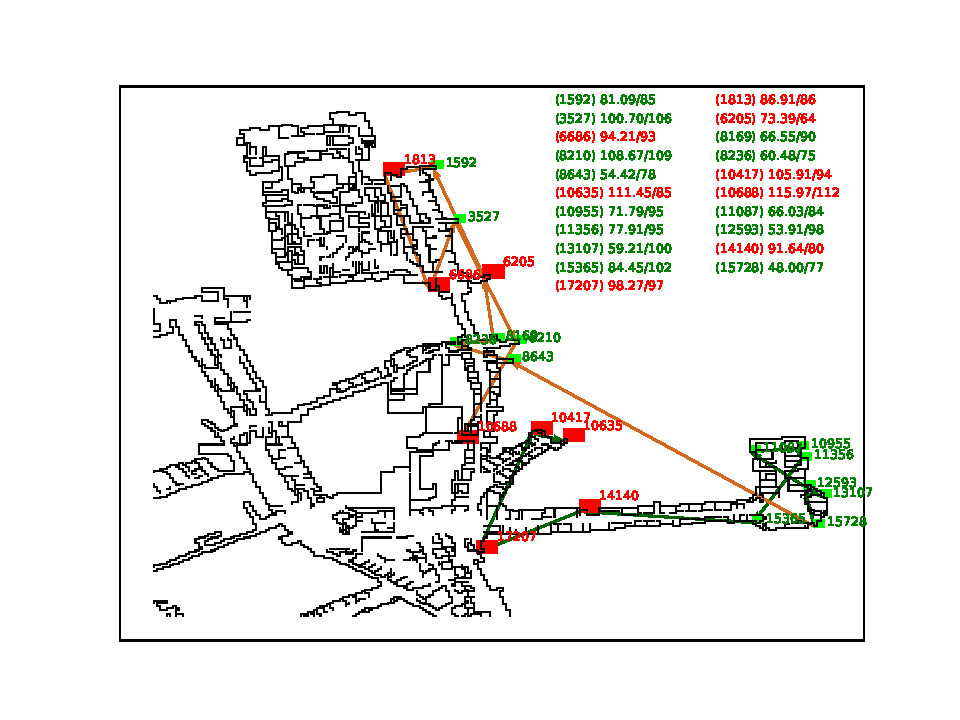
\includegraphics[width=5cm,trim=100 50 100 50]{fig/43min_2team_nolim.pdf}
    \caption{設置開始時刻 43 分,\newline \quad 設置チーム数 2,稼働時間
    上限なし}
    \label{fig:43min_2team_nolim}
   \end{center}
  \end{minipage}
  %
  \begin{minipage}{0.49\hsize}
   \begin{center}
    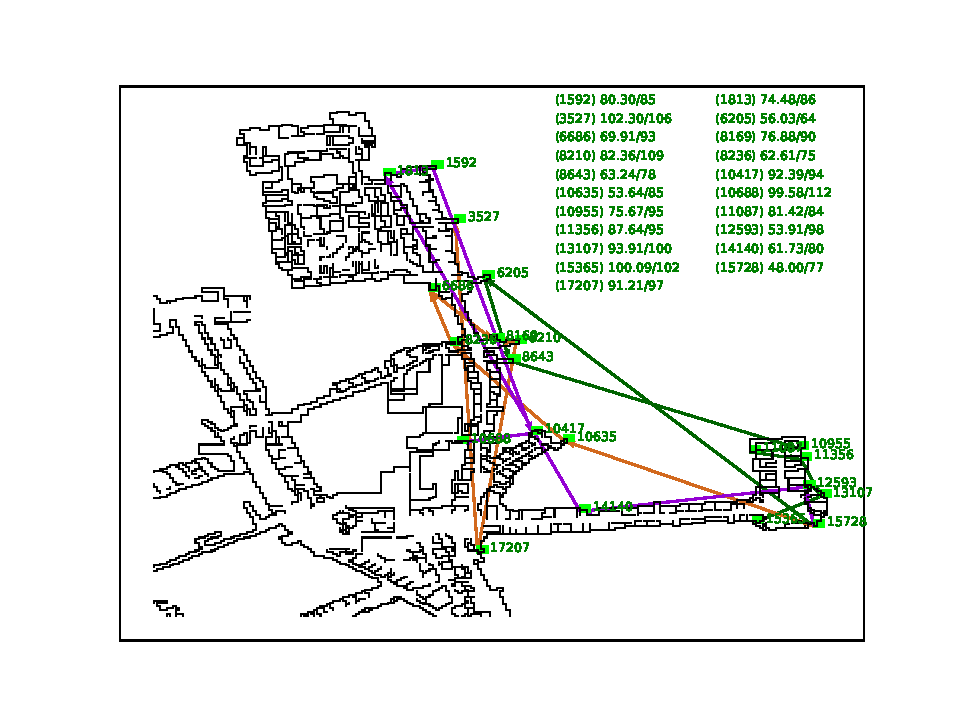
\includegraphics[width=5cm,trim=100 50 100 50]{fig/43min_3team_nolim.pdf}
    \caption{設置開始時刻 43 分,\newline \quad 設置チーム数 3,稼働時間上限なし}
    \label{fig:43min_3team_nolim}
   \end{center}
  \end{minipage}
  %
 \end{center}
\end{figure}

\begin{figure}
 \begin{center}
  %
  \begin{minipage}{0.49\hsize}
   \begin{center}
    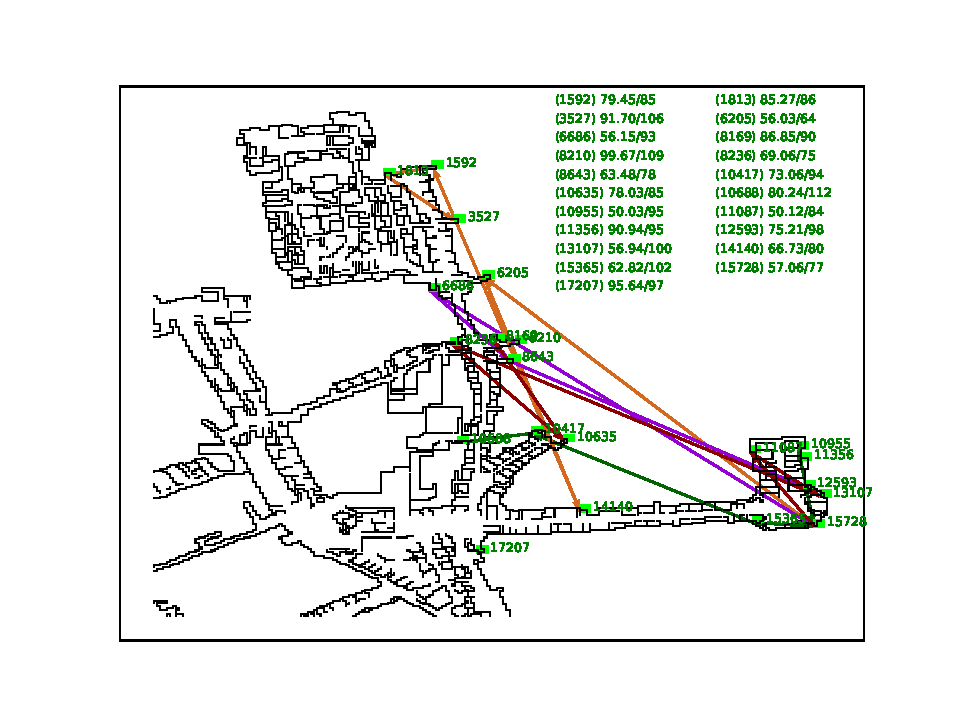
\includegraphics[width=5cm,trim=100 50 100 50]{fig/43min_4team_nolim.pdf}
    \caption{設置開始時刻 43 分,\newline \quad 設置チーム数 4,稼働時間上限なし}
    \label{fig:43min_4team_nolim}
   \end{center}
  \end{minipage}
  %
  \begin{minipage}{0.49\hsize}
   \begin{center}
    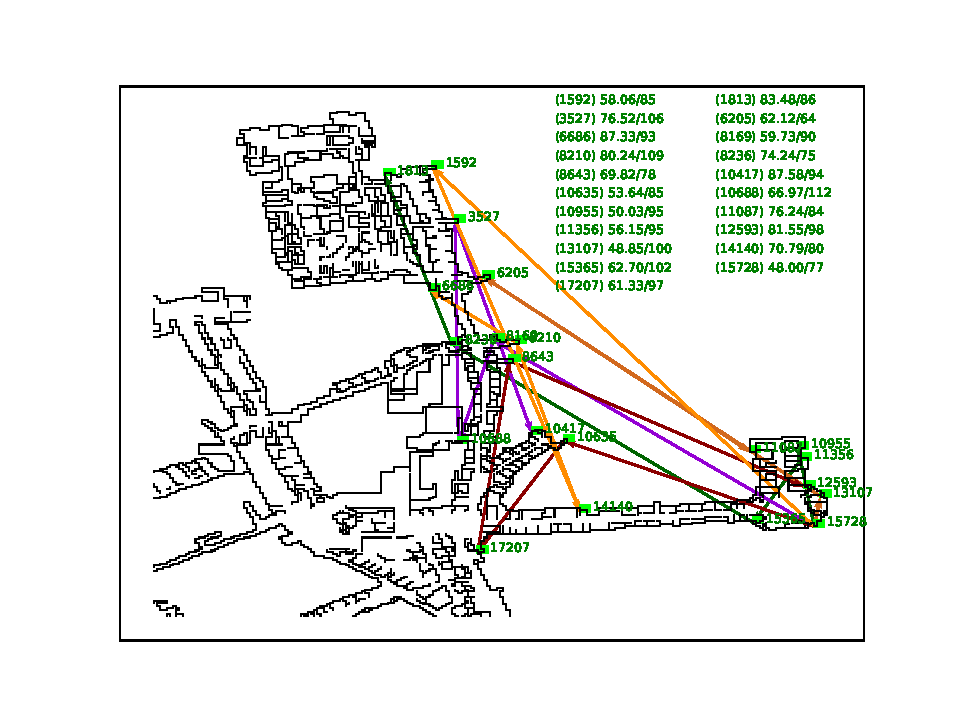
\includegraphics[width=5cm,trim=100 50 100 50]{fig/43min_5team_nolim.pdf}
    \caption{設置開始時刻 43 分,\newline \quad 設置チーム数 5,稼働時間上限なし}
    \label{fig:43min_5team_nolim}
   \end{center}
  \end{minipage}
  %
 \end{center}
\end{figure}

\begin{figure}
 \begin{center}
  %
  \begin{minipage}{0.49\hsize}
   \begin{center}
    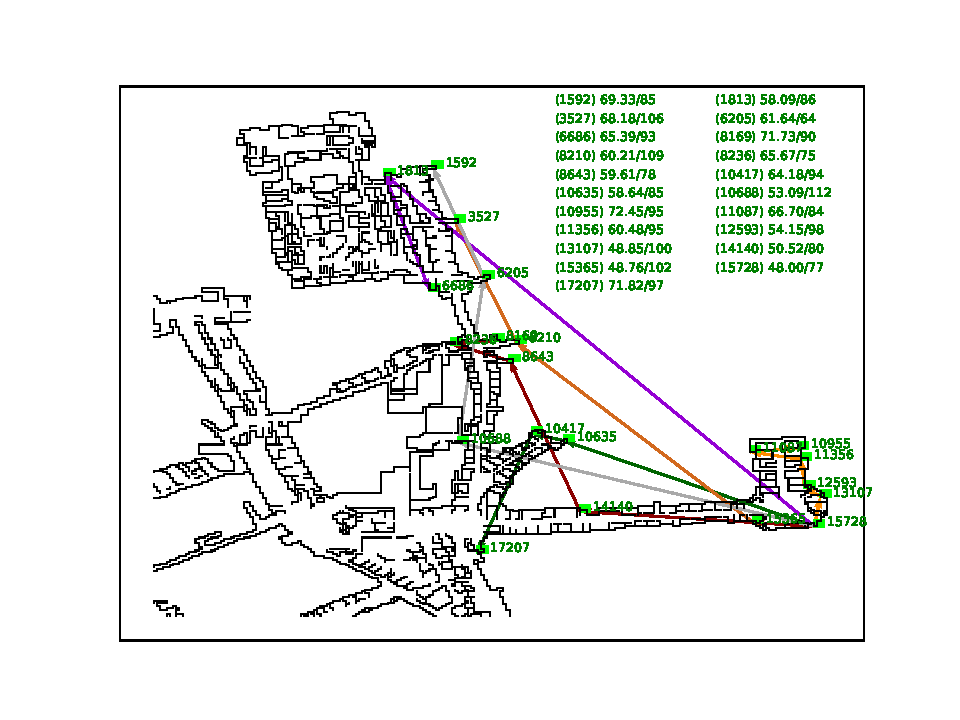
\includegraphics[width=5cm,trim=100 50 100 50]{fig/43min_6team_lim30min.pdf}
    \caption{設置開始時刻 43 分,\newline \quad 設置チーム数 6,稼働時間上限 30 分}
    \label{fig:43min_6team_lim30min}
   \end{center}
  \end{minipage}
  %
  \begin{minipage}{0.49\hsize}
   \begin{center}
    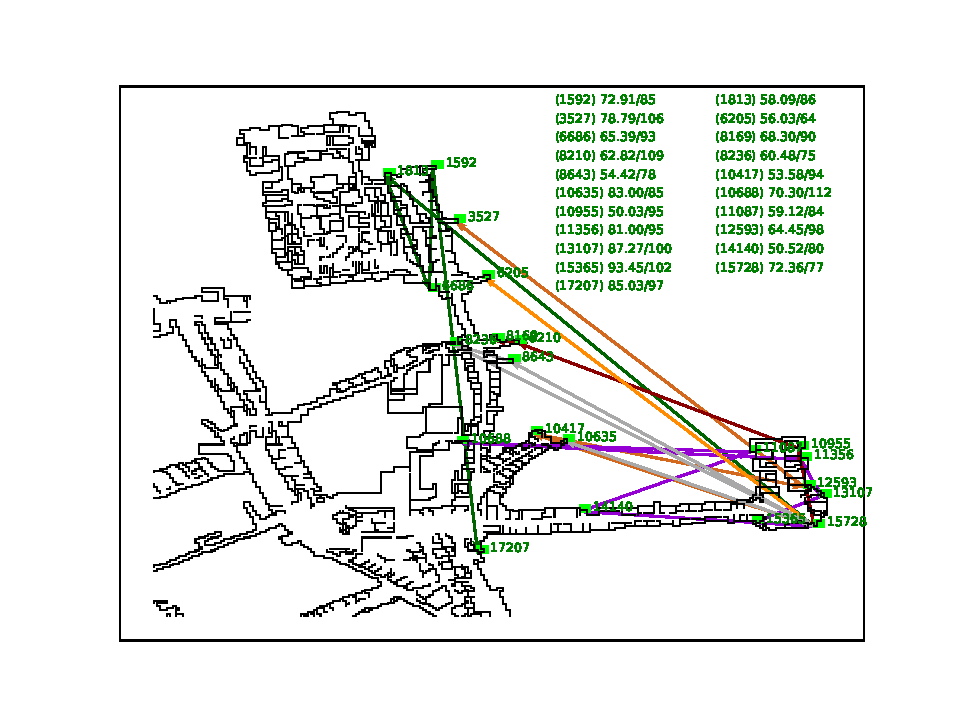
\includegraphics[width=5cm,trim=100 50 100 50]{fig/43min_6team_nolim.pdf}
    \caption{設置開始時刻 43 分,\newline \quad 設置チーム数 6,稼働時間上限なし}
    \label{fig:43min_6team_nolim}
   \end{center}
  \end{minipage}
  %
 \end{center}
\end{figure}

\begin{figure}
 \begin{center}
  %
  \begin{minipage}{0.49\hsize}
   \begin{center}
    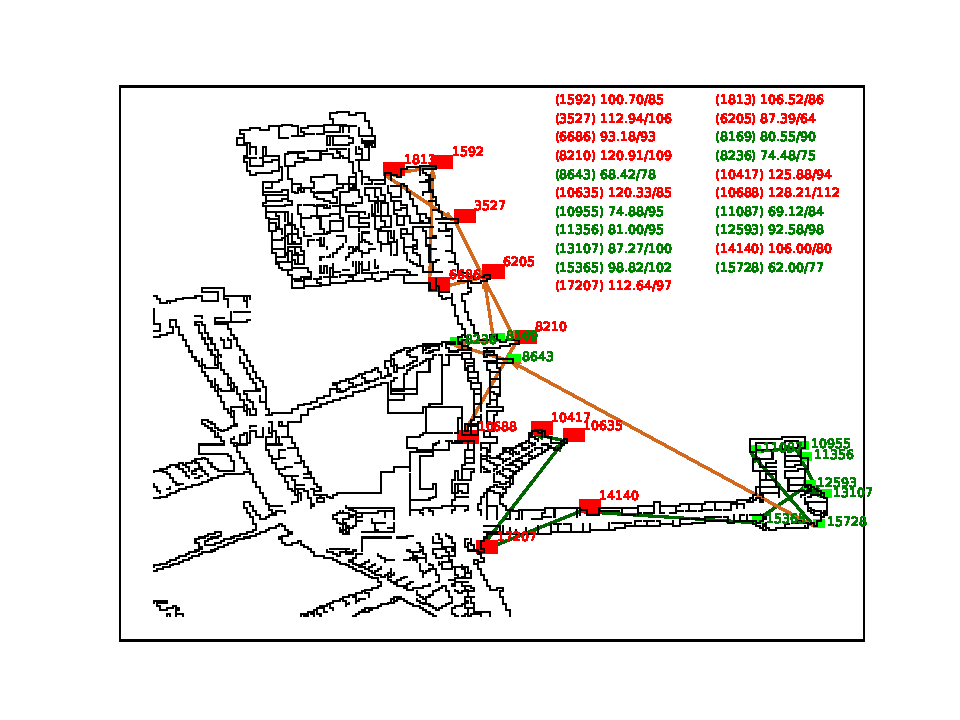
\includegraphics[width=5cm,trim=100 50 100 50]{fig/57min_2team_nolim.pdf}
    \caption{設置開始時刻 57 分,\newline \quad 設置チーム数 2,稼働時間上限なし}
    \label{fig:57min_2team_nolim}
   \end{center}
  \end{minipage}
  %
  \begin{minipage}{0.49\hsize}
   \begin{center}
    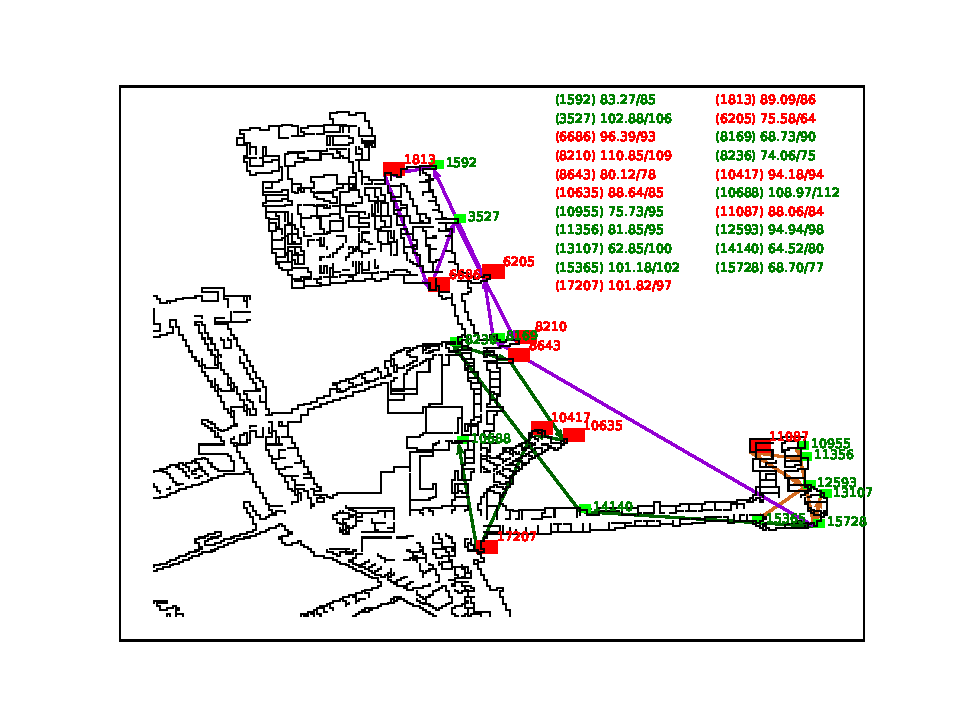
\includegraphics[width=5cm,trim=100 50 100 50]{fig/57min_3team_nolim.pdf}
    \caption{設置開始時刻 57 分,\newline \quad 設置チーム数 3,稼働時間上限なし}
    \label{fig:57min_3team_nolim}
   \end{center}
  \end{minipage}
  %
 \end{center}
\end{figure}

\begin{figure}
 \begin{center}
  %
  \begin{minipage}{0.49\hsize}
   \begin{center}
    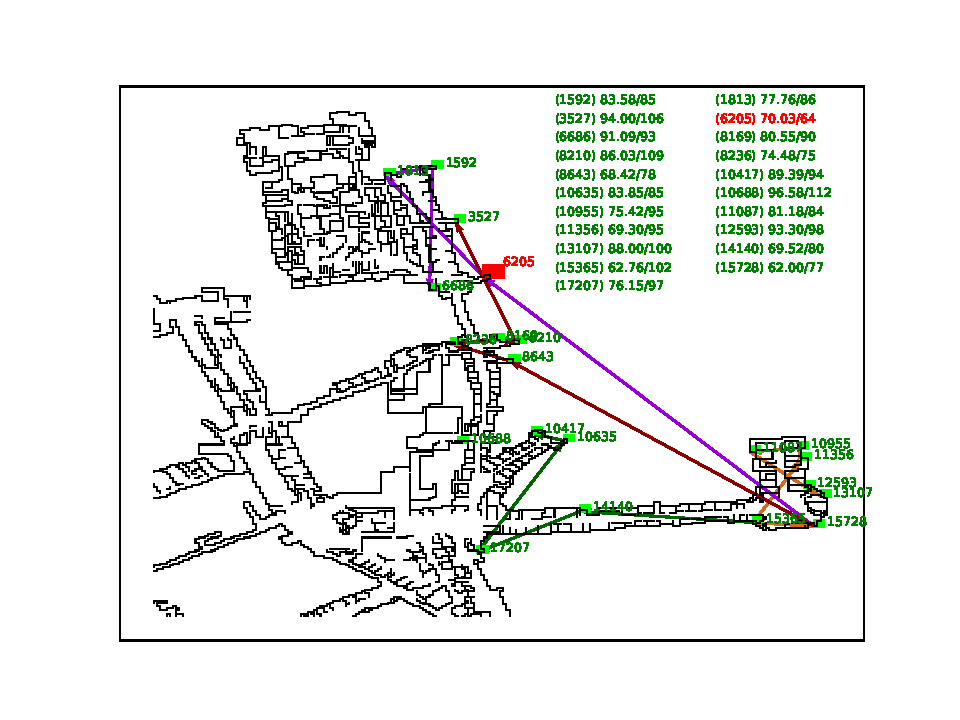
\includegraphics[width=5cm,trim=100 50 100 50]{fig/57min_4team_lim40min.pdf}
    \caption{設置開始時刻 57 分,\newline \quad 設置チーム数 4,稼働時間上限 40 分}
    \label{fig:57min_4team_lim40min}
   \end{center}
  \end{minipage}
  %
  \begin{minipage}{0.49\hsize}
   \begin{center}
    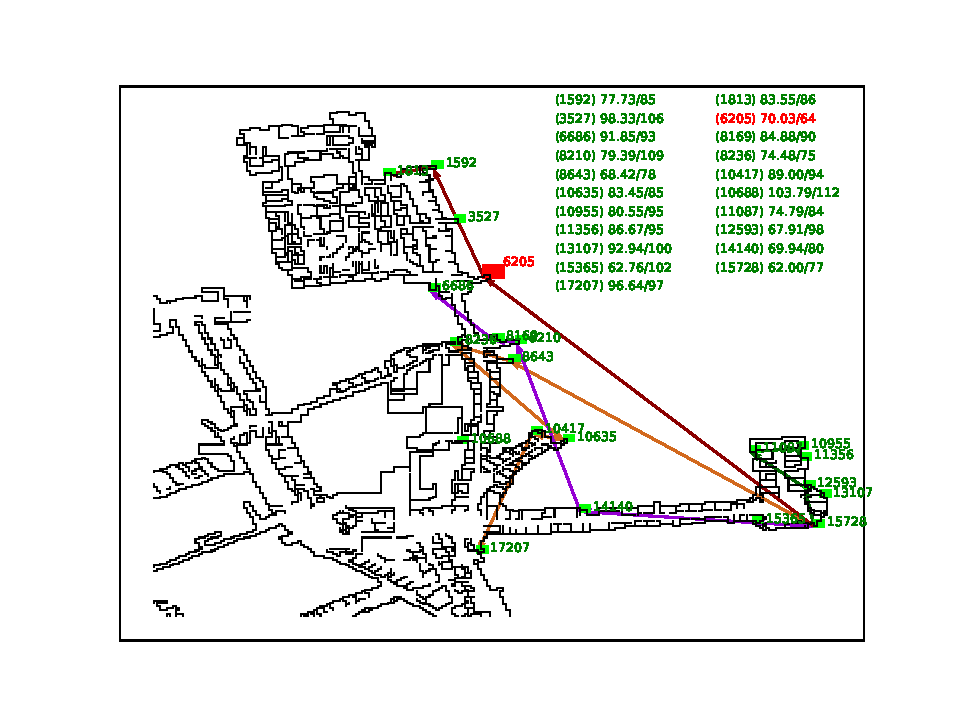
\includegraphics[width=5cm,trim=100 50 100 50]{fig/57min_4team_nolim.pdf}
    \caption{設置開始時刻 57 分,\newline \quad 設置チーム数 4,稼働時間上限なし}
    \label{fig:57min_4team_nolim}
   \end{center}
  \end{minipage}
  %
 \end{center}
\end{figure}

\begin{figure}
 \begin{center}
  %
  \begin{minipage}{0.49\hsize}
   \begin{center}
    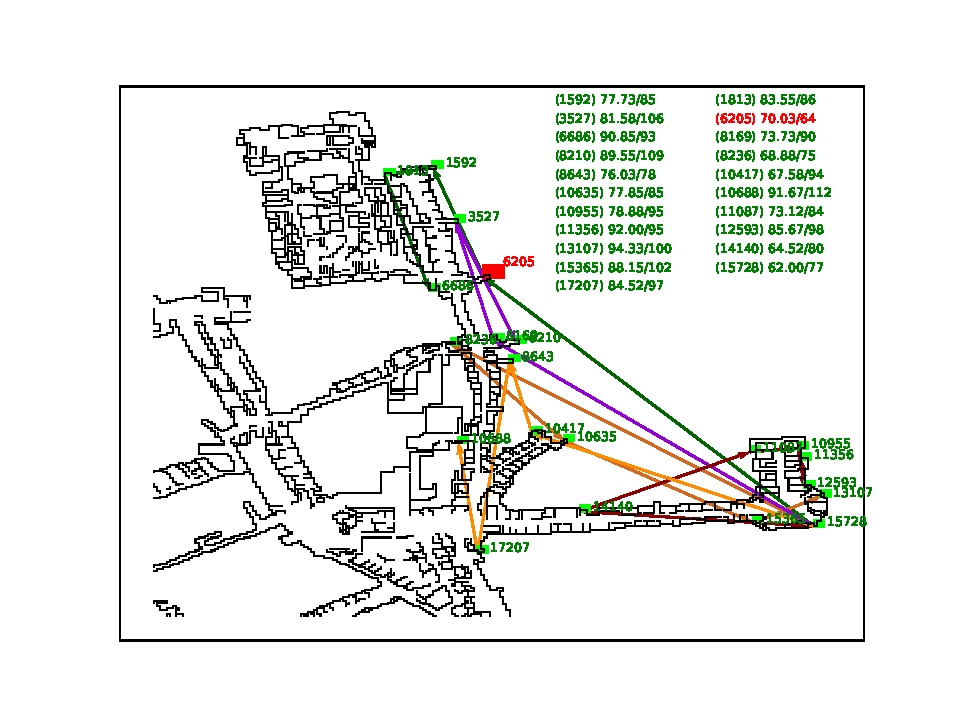
\includegraphics[width=5cm,trim=100 50 100 50]{fig/57min_5team_lim40min.pdf}
    \caption{設置開始時刻 57 分,\newline \quad 設置チーム数 5,稼働時間上限 40 分}
    \label{fig:57min_5team_lim40min}
   \end{center}
  \end{minipage}
  %
  \begin{minipage}{0.49\hsize}
   \begin{center}
    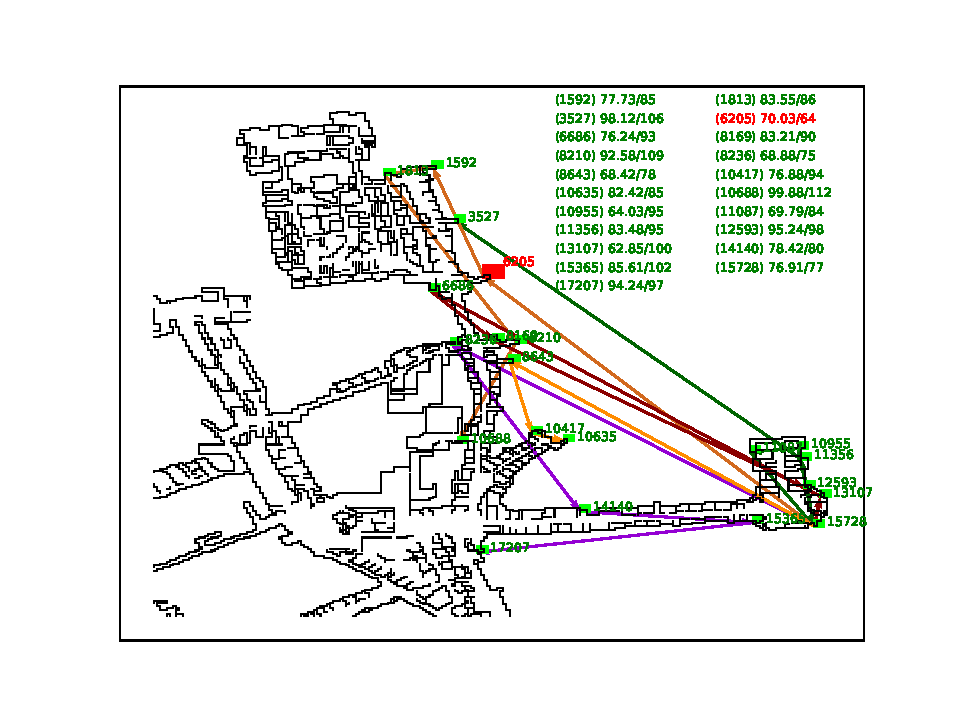
\includegraphics[width=5cm,trim=100 50 100 50]{fig/57min_5team_nolim.pdf}
    \caption{設置開始時刻 57 分,\newline \quad 設置チーム数 5,稼働時間上限なし}
    \label{fig:57min_5team_nolim}
   \end{center}
  \end{minipage}
  %
 \end{center}
\end{figure}

\begin{figure}
 \begin{center}
  %
  \begin{minipage}{0.49\hsize}
   \begin{center}
    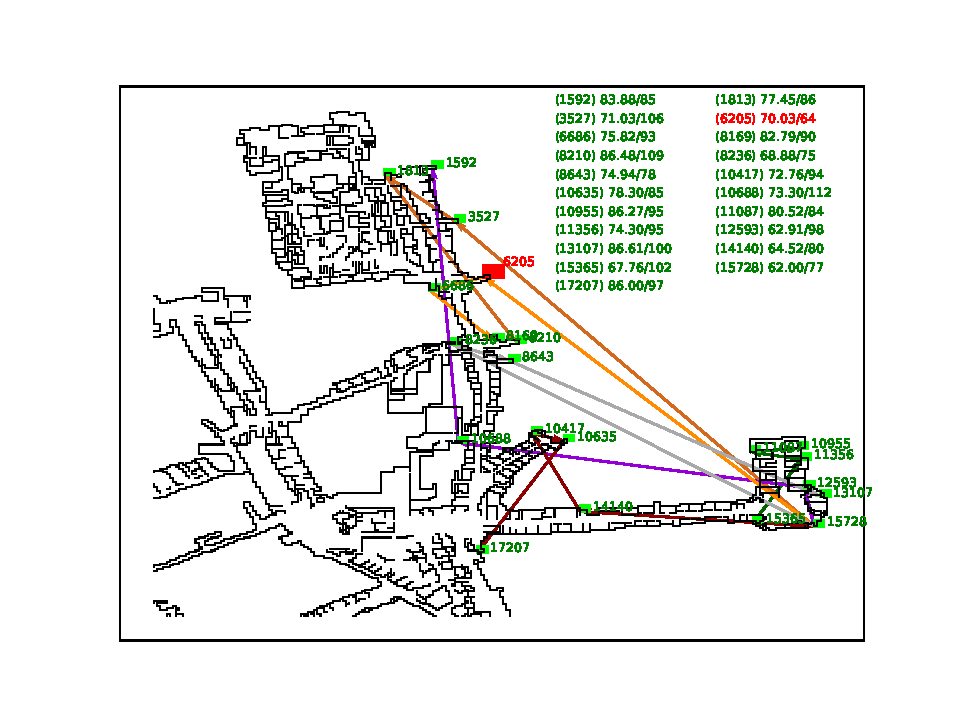
\includegraphics[width=5cm,trim=100 50 100 50]{fig/57min_6team_lim30min.pdf}
    \caption{設置開始時刻 57 分,\newline \quad 設置チーム数 6,稼働時間上限 30 分}
    \label{fig:57min_6team_lim30min}
   \end{center}
  \end{minipage}
  %
  \begin{minipage}{0.49\hsize}
   \begin{center}
    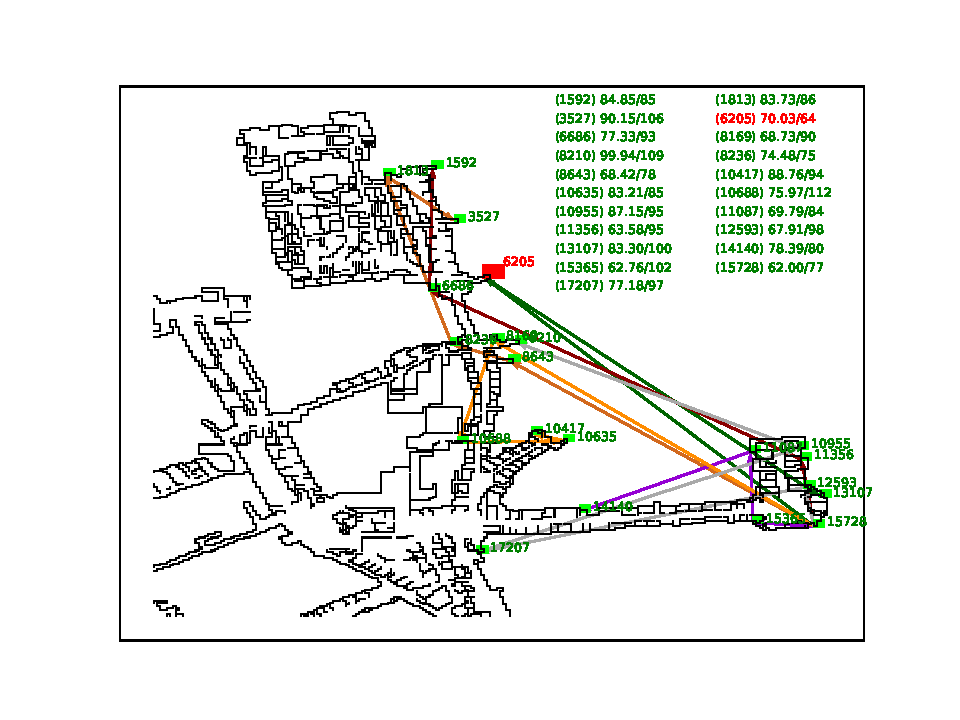
\includegraphics[width=5cm,trim=100 50 100 50]{fig/57min_6team_nolim.pdf}
    \caption{設置開始時刻 57 分,\newline \quad 設置チーム数 6,稼働時間上限なし}
    \label{fig:57min_6team_nolim}
   \end{center}
  \end{minipage}
  %
 \end{center}
\end{figure}

\begin{figure}
 \begin{center}
  %
  \begin{minipage}{0.49\hsize}
   \begin{center}
    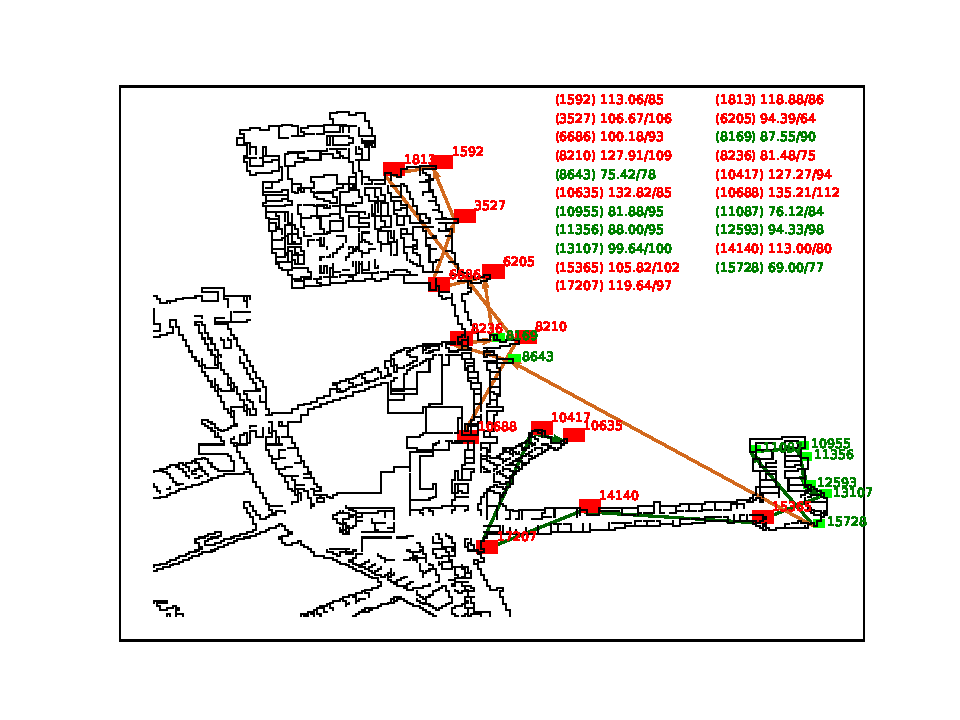
\includegraphics[width=5cm,trim=100 50 100 50]{fig/64min_2team_nolim.pdf}
    \caption{設置開始時刻 64 分,\newline \quad 設置チーム数 2,稼働時間上限なし}
    \label{fig:64min_2team_nolim}
   \end{center}
  \end{minipage}
  %
  \begin{minipage}{0.49\hsize}
   \begin{center}
    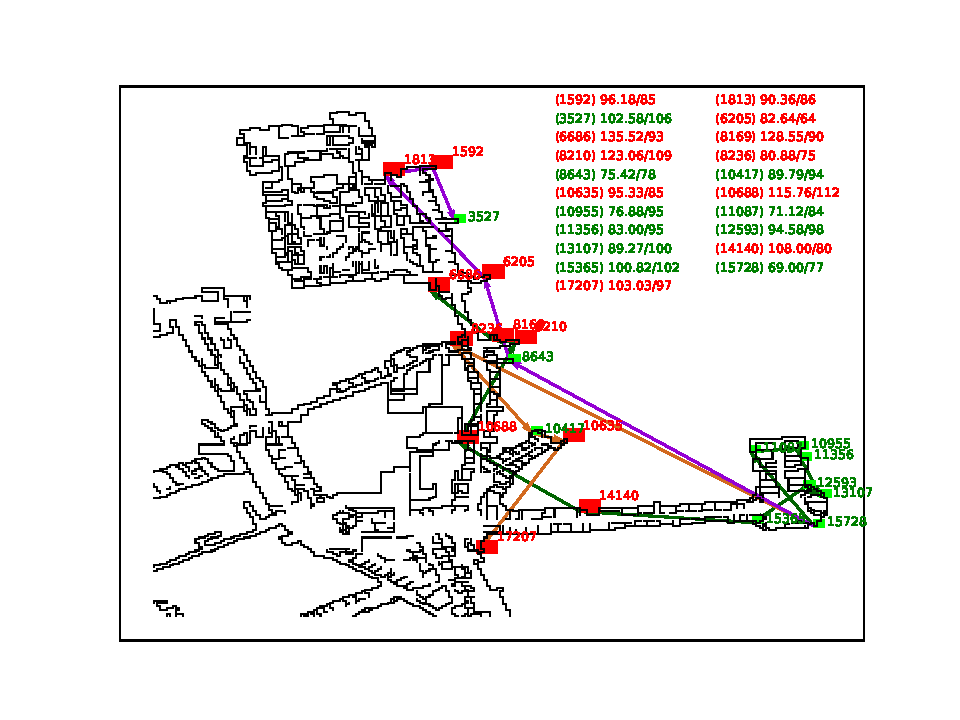
\includegraphics[width=5cm,trim=100 50 100 50]{fig/64min_3team_lim40min.pdf}
    \caption{設置開始時刻 64 分,\newline \quad 設置チーム数 3,稼働時間上限 40 分}
    \label{fig:64min_3team_lim40min}
   \end{center}
  \end{minipage}
  %
 \end{center}
\end{figure}

\begin{figure}
 \begin{center}
  %
  \begin{minipage}{0.49\hsize}
   \begin{center}
    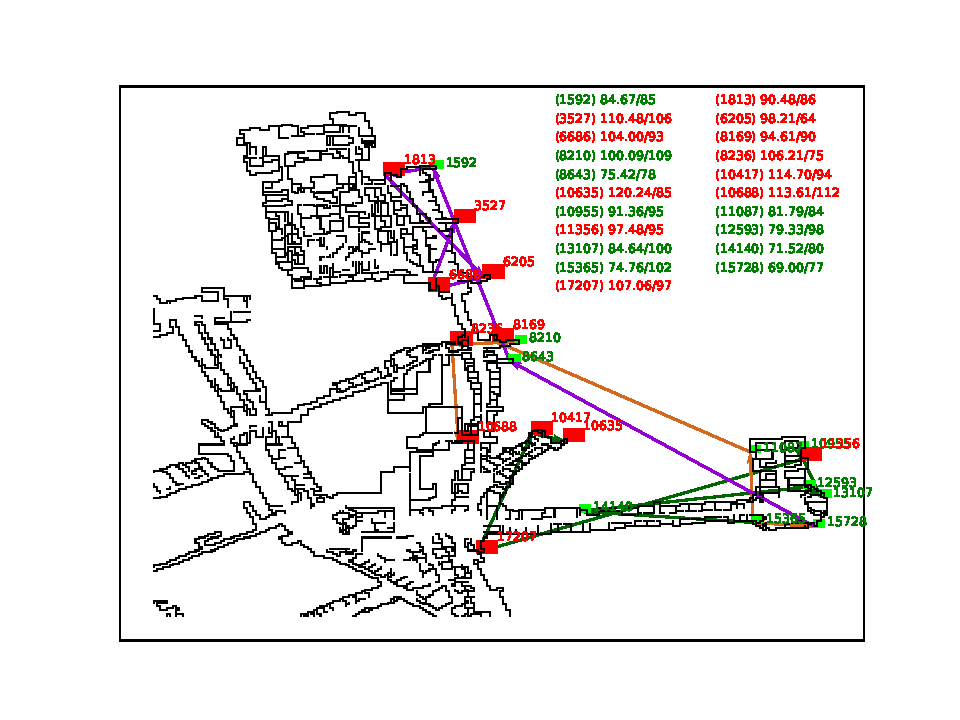
\includegraphics[width=5cm,trim=100 50 100 50]{fig/64min_3team_lim50min.pdf}
    \caption{設置開始時刻 64 分,\newline \quad 設置チーム数 3,稼働時間上限 50 分}
    \label{fig:64min_3team_lim50min}
   \end{center}
  \end{minipage}
  %
  \begin{minipage}{0.49\hsize}
   \begin{center}
    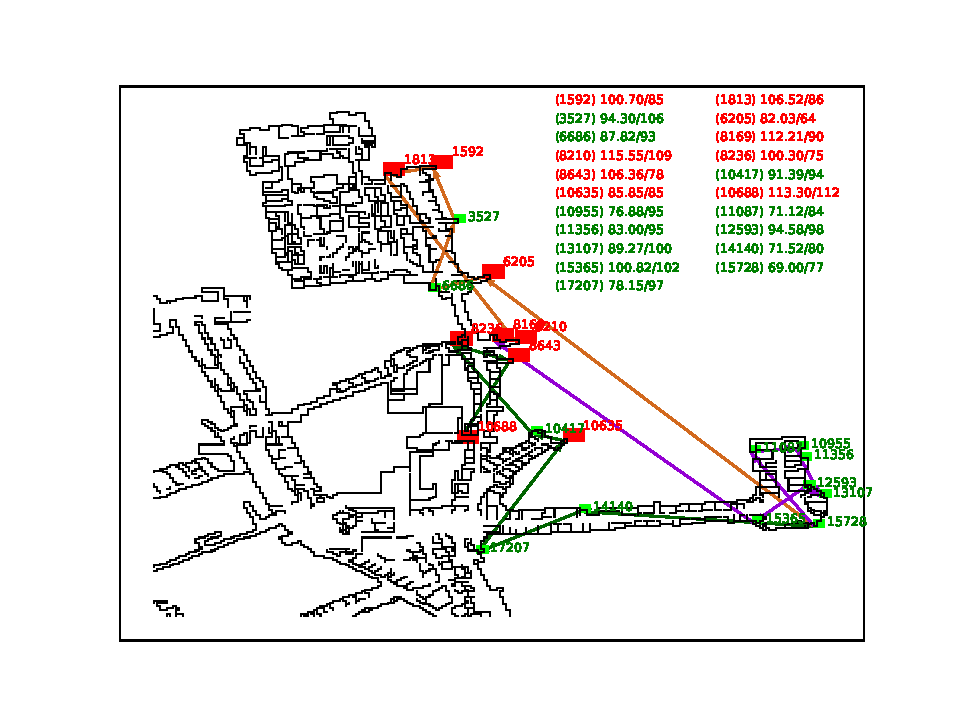
\includegraphics[width=5cm,trim=100 50 100 50]{fig/64min_3team_nolim.pdf}
    \caption{設置開始時刻 64 分,\newline \quad 設置チーム数 3,稼働時間上限なし}
    \label{fig:64min_3team_nolim}
   \end{center}
  \end{minipage}
  %
 \end{center}
\end{figure}

\begin{figure}
 \begin{center}
  %
  \begin{minipage}{0.49\hsize}
   \begin{center}
    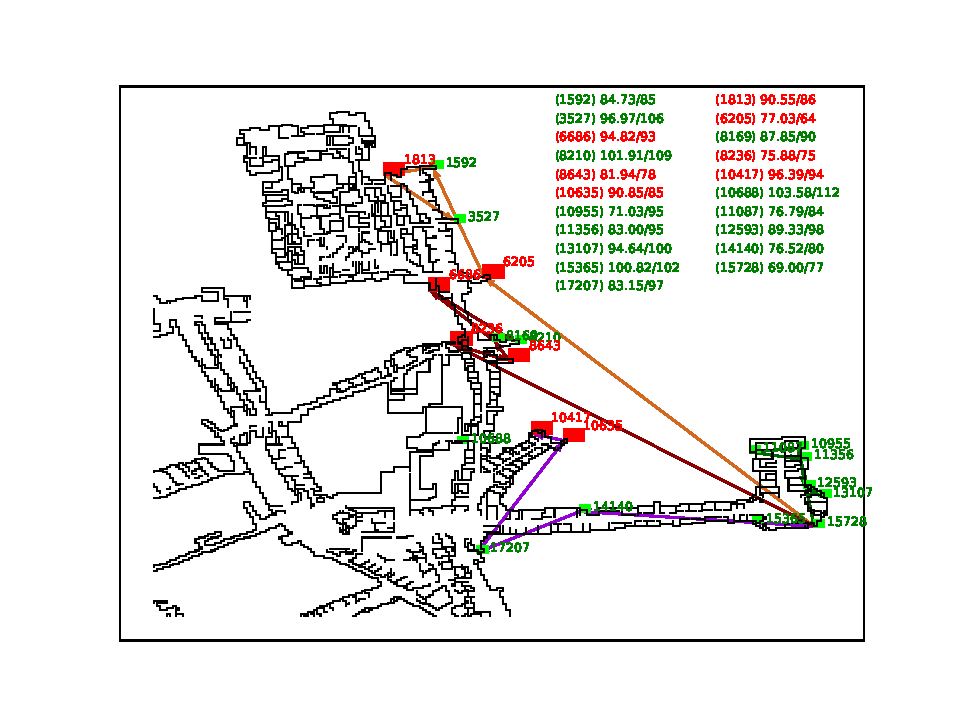
\includegraphics[width=5cm,trim=100 50 100 50]{fig/64min_4team_lim40min.pdf}
    \caption{設置開始時刻 64 分,\newline \quad 設置チーム数 4,稼働時間上限 40 分}
    \label{fig:64min_4team_lim40min}
   \end{center}
  \end{minipage}
  %
  \begin{minipage}{0.49\hsize}
   \begin{center}
    \includegraphics[width=5cm,trim=100 50 100 50]{fig/64min_4team_nolim.pdf}
    \caption{設置開始時刻 64 分,\newline \quad 設置チーム数 4,稼働時間上限なし}
    \label{fig:64min_4team_nolim}
   \end{center}
  \end{minipage}
  %
 \end{center}
\end{figure}

\begin{figure}
 \begin{center}
  %
  \begin{minipage}{0.49\hsize}
   \begin{center}
    \includegraphics[width=5cm,trim=100 50 100 50]{fig/64min_5team_lim40min.pdf}
    \caption{設置開始時刻 64 分,\newline \quad 設置チーム数 5,稼働時間上限 40 分}
    \label{fig:64min_5team_lim40min}
   \end{center}
  \end{minipage}
  %
  \begin{minipage}{0.49\hsize}
   \begin{center}
    \includegraphics[width=5cm,trim=100 50 100 50]{fig/64min_5team_nolim.pdf}
    \caption{設置開始時刻 64 分,\newline \quad 設置チーム数 5,稼働時間上限なし}
    \label{fig:64min_5team_nolim}
   \end{center}
  \end{minipage}
  %
 \end{center}
\end{figure}

\begin{figure}
 \begin{center}
  %
  \begin{minipage}{0.49\hsize}
   \begin{center}
    \includegraphics[width=5cm,trim=100 50 100 50]{fig/64min_6team_lim30min.pdf}
    \caption{設置開始時刻 64 分,\newline \quad 設置チーム数 6,稼働時間上限 30 分}
    \label{fig:64min_6team_lim30min}
   \end{center}
  \end{minipage}
  %
  \begin{minipage}{0.49\hsize}
   \begin{center}
    \includegraphics[width=5cm,trim=100 50 100 50]{fig/64min_6team_nolim.pdf}
    \caption{設置開始時刻 64 分,\newline \quad 設置チーム数 6,稼働時間上限なし}
    \label{fig:64min_6team_nolim}
   \end{center}
  \end{minipage}
  %
 \end{center}
\end{figure}

\newpage

\begin{table}
\begin{center}
\caption{各実験における目的関数値等}
\label{tb:experiment_summary}
\scalebox{0.8}{
 \begin{tabular}{ccc|r|rr}\hline
  設置開始時刻(分) & 設置チーム数 & 稼働時間上限(分) & 流入時間合計(分) & 計算時間(秒) & GAP(\%) \\ \hline
  43 & 2 & 設定なし & 66.76  & 3600.06 & 100.00 \\ \hline
  43 & 3 & 設定なし & 0.00   & 3186.69 & -- \\ \hline
  43 & 4 & 設定なし & 0.00   & 4.64    & -- \\ \hline
  43 & 5 & 設定なし & 0.00   & 402.29  & -- \\ \hline
  43 & 6 & 30       & 0.00   & 31.45   & -- \\ \hline
  43 & 6 & 設定なし & 0.00   & 230.62  & -- \\ \hline
  57 & 2 & 設定なし & 203.70 & 3600.28 & 100.00 \\ \hline
  57 & 3 & 設定なし & 34.73  & 3600.08 & 100.00 \\ \hline
  57 & 4 & 40       & 6.03   & 539.69  & -- \\ \hline
  57 & 4 & 設定なし & 6.03   & 427.98  & -- \\ \hline
  57 & 5 & 40       & 6.03   & 171.66  & -- \\ \hline
  57 & 5 & 設定なし & 6.03   & 89.58   & -- \\ \hline
  57 & 6 & 30       & 6.03   & 409.37  & -- \\ \hline
  57 & 6 & 設定なし & 6.03   & 59.94   & -- \\ \hline
  64 & 2 & 設定なし & 288.33 & 3600.09 & -- \\ \hline
  64 & 3 & 40       & 183.30 & 3600.08 & 96.84 \\ \hline
  64 & 3 & 50       & 160.09 & 3600.35 & 96.88 \\ \hline
  64 & 3 & 設定なし & 138.82 & 3600.14 & 96.40 \\ \hline
  64 & 4 & 40       & 32.45  & 3600.08 & 59.85 \\ \hline
  64 & 4 & 設定なし & 24.21  & 3600.03 & 46.18 \\ \hline
  64 & 5 & 40       & 13.91  & 1300.32 & -- \\ \hline
  64 & 5 & 設定なし & 13.91  & 939.54  & -- \\ \hline
  64 & 6 & 30       & 13.91  & 1540.24 & -- \\ \hline
  64 & 6 & 設定なし & 13.91  & 588.00  & -- \\ \hline
 \end{tabular}
}
\end{center}
\end{table}

%%%%%%%%%%%%%%%%%%%%%%%%%%%%%%%%%%%%%%%%%%%%%%%%%%%%%%%%%%%%%%%%%%%%%%
\end{document}
%%%%% End of file %%%%%
